\documentclass[
draft%     uncomment to activate draft mode (see preamble/proofs)
]{article}   

% preamble -- do not rearrange order of \includes
%\include{classoptions}
%\include{pagesize}
%\include{packages}
%\include{encoding}         
%\include{fonts}
%\include{ToC}
%\include{contributor}
%\include{copyright}
%\include{bibtex}
%\include{environments}
%\include{sectionoptions}
%\include{headerfooter}
%\include{footnoteformat}
%\include{codesnipets}
%\include{proofs}

\usepackage{tikz}
\usepackage{graphicx}
\usepackage[export]{adjustbox}
\usepackage{caption}
\usetikzlibrary{shapes}
\usetikzlibrary {positioning}

\usepackage{geometry}
\usepackage{array}
\usepackage{hyperref}
\hypersetup{
    colorlinks=true,
    linkcolor=magenta,
    filecolor=cyan,      
    urlcolor=blue,
}
\graphicspath{ {./images/} }

% define issue details
\title{Compiler Optimization Notes}
\newcommand\thejournalsubtitle{Notes compiled for the Compiler Optimization Course}
\newcommand\thevolume{}
\newcommand\theseason{February}
\newcommand\theyear{2021}
\newcommand\theissue{\thejournal \ \thevolume \ (\theyear)} 
\newcommand\generaleditor{}
\newcommand\associateeditor{}
\sloppy
\newcommand\thewebsite{https://iitd.github.io/col729}

\begin{document}
\sloppy                         % preferences more space between words over overrunning margins
\lefthyphenmin=3                % suppresses hyphenation after only 1 or 2 characters
                                % NB: You will need to repeat \lefthyphenmin in the text if you use \selectlanguage
%\include{editorialboard}
%\include{titlepage}
%\include{colofon}
\pagenumbering{roman}           
%\tableofcontents  
\thispagestyle{empty}

% \include{essays/preface}
\pagenumbering{arabic}
%\part{COL729 Lecture Modules and Discussions}
% \section{Intermediate Representation}

\section{Three Address Code}
 
%\section{Module 70 : Static Single Assignment IR}
Consider the following example

    \[x = y+z\]
    \[x = x+1\]
    \[w=y+z\]
    \[z=x+3\]
    
In this example, the computation $y+z$ could be reused.
In SSA, we assign versions to variables(as below) and each version has only one assignment to it. SSA stands for single assignment in a static program. 
    \[x_1 = y+z\]
    \[x_2 = x_1+1\]
    \[w_1=y+z\]
    \[v_1=x_2+3\]
    
Using SSA, we can not optimize the code by rewriting $w_1 = y+z$ as $w_1 = x_1$.

    \[x_1 = y+z\]
    \[x_2 = x_1+1\]
    \[w_1=x_1\]
    \[v_1=x_2+3\]
    
Why SSA? Advantages of SSA:
\begin{itemize}
    \item Optimization algorithms become simpler if each variable has only one definition.
    \item Unrelated uses of same variable become independent.
    \item More values become available at each program point.
\end{itemize}
Therefore, SSA is a very popular method of IR design. LLVM IR is also an SSA IR.

\subsection{Converting to SSA}
\begin{itemize}
    \item Replace the target of each assignment with a new variable.
    \item Replace each use of a variable with the version of the variable reaching that point.
\end{itemize}
Again, taking an example:

    \[x = y+z\]
    \[a = b+x\]
    \[x=a+3\]
    \[y=x-a\]
On applying the two rules for conversion to SSA, these statements change to :
     \[x_1 = y+z\]
    \[a = b+x_1\]
    \[x_2=a+3\]
    \[y=x_2-a\]
    

\begin{figure*}
\centering
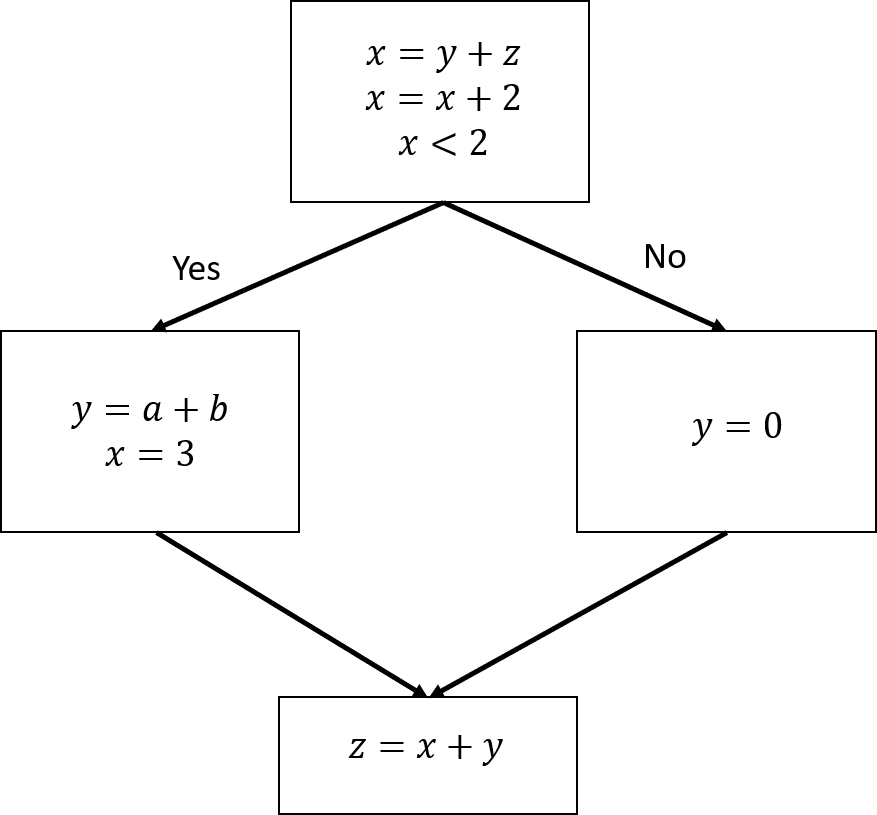
\includegraphics[height=8cm]{images/Example1.png}
\caption{Converting to SSA Example}
\end{figure*}

Consider another example as shown in Figure 1:

In this example, there are 2 variables of interest. $x$ is assigned thrice and $y$ is assigned thrice. On applying the rules of SSA conversion, here is how the code snippet looks like.

The versioning is straightforward for variable $x$. For $y$ in this example, there are two versions reaching at the bottom block from two different paths. The question is how we version the variable $y$ at bottom block. To answer that , we need to understand about basic block
\begin{figure*}
\centering
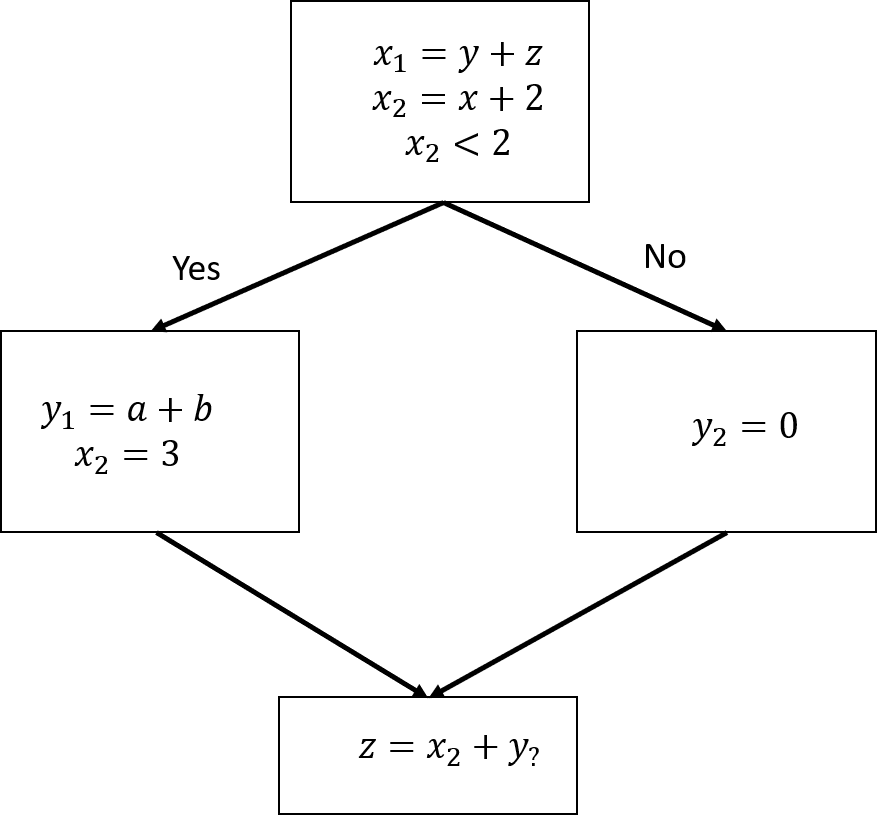
\includegraphics[height=8cm]{images/Example2.png}
\caption{Converting to SSA Example - With Versions}
\end{figure*}

\subsection{Basic Block}: 
A basic block is a maximal set of instructions with 
\begin{itemize}
    \item no labels( except at the first instruction)
    \item no jumps (except in the last instruction)
\end{itemize}

In the example, each rectangle is a basic block. 
Idea:
\begin{itemize}
    \item Cannot jump into a basic block (except at beginning)
    \item cannot jump out of a basic block (except at end)
    \item Single-entry single-exit straight line code segment
\end{itemize}

At the bottom block, there are two version reaching for variable $y$. To represent that we use $\Phi$ node or $\Phi$ function. So the version of y can be represented as a function of $y_1$ and $y_2$ as shown in figure XXX. This is an ordered set.


\begin{figure*}
\centering
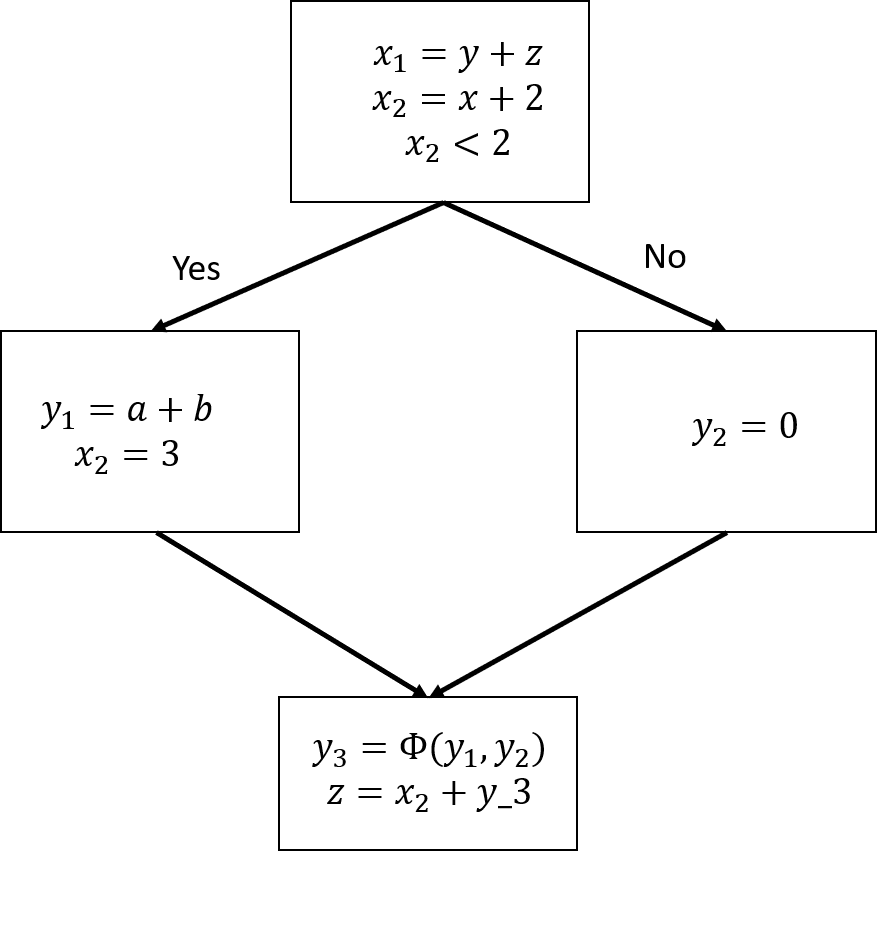
\includegraphics[height=8cm]{images/Example3.png}
\caption{Converting to SSA Example - PHI Nodes}
\end{figure*} 

\subsection{PHI($\Phi$) Nodes}
\begin{itemize}
    \item $\Phi$ function chooses the version depending on the incoming edge.
    \item Present only at the beginning of a basic block. Since this is the only place where there are multiple versions flowing through different incoming edges.
\end{itemize}


%\section{Phi Nodes}

In SSA IR, we encountered the issue of figuring out which variable version to use after a join point where multiple paths were coming in with different versions of the same variable. As a solution to this, phi nodes or phi functions are extremely helpful that could be placed only at the beginning of a basic block with multiple edges coming in (join point).

These phi nodes can be placed at each join point for every variable in the program. This placement strategy is a bit wasteful as illustrated in the following diagram:

\begin{figure}[htp]
\centering
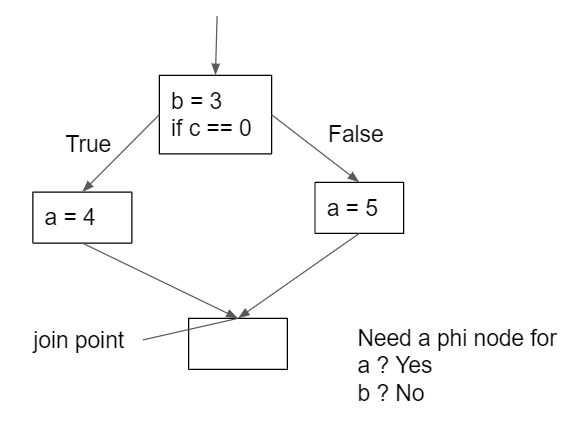
\includegraphics[height=6cm]{images/phinodes.png}
\caption{Placement of \(\Phi\) nodes}
\end{figure}

\subsection{Path Convergence Criterion}

Consider z to be node with multiple edges coming in (thus it is a join point). We need \(\Phi\) node for variable a at node z if and only if
\begin{enumerate}
    \item There is a block x containing the definition of a.
    \item There is a block y (not x) containing the definition of a.
    \item There are non empty paths \(P_{xz}\) and \(P_{yz}\) from x to z and y to z respectively.
            \begin{figure}[htp]
\centering
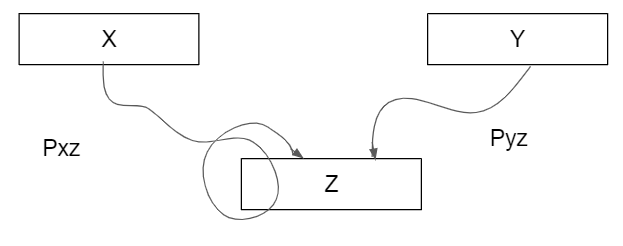
\includegraphics[height=3cm]{images/Condition123.png}
\caption{CFG for condition 1, 2, 3}
\end{figure}
    \item \(P_{xz}\) and \(P_{yz}\) should not have any node in common except z.
        \begin{figure}[htp]
\centering
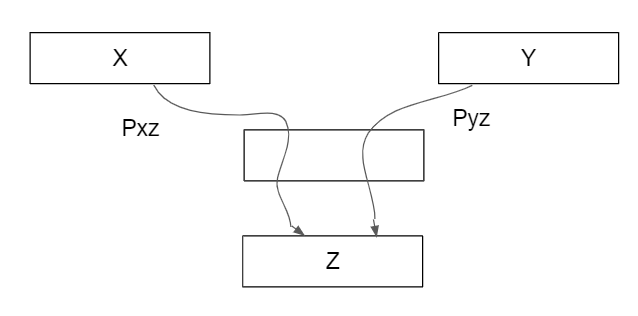
\includegraphics[height=3cm]{images/Condtion4.png}
\caption{Violation of Condition 4}
\end{figure}
    \item The node z does not appear within both  \(P_{xz}\) and \(P_{yz}\), prior to the end. It is fine if z appears only in one of the path before end.
            \begin{figure}[htp]
\centering
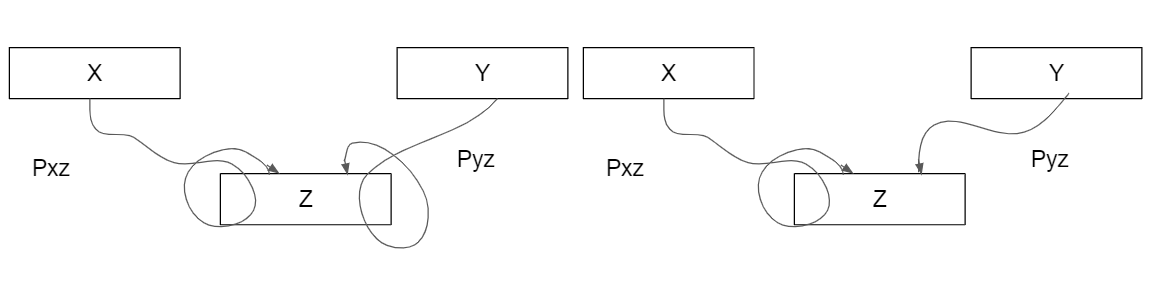
\includegraphics[height=3cm]{images/Condition5.png}
\caption{Cpndition 5: Left CFG does not need \(\Phi\) node, right CFG needs \(\Phi\) node}
\end{figure}
\end{enumerate}

\subsection{Iterative Fixed Point Algorithm}

while \{there are nodes x, y, z satisfying condition 1-5 and z does not contain a \(\Phi\) node for a\}\\
do \{insert \(a \leftarrow \Phi(a_1, a_2, ..., a_j)\) \}

The \(\Phi\) function has as many 'a' arguments as there are predecessors of z. Since the conditions 1-5 are both sufficient and necessary, the above algorithm is sound and complete.
 
\section{Optimization Overview}

Most intermediate representations are organised as \textit{control flow graphs (CFG)} over \textit{basic blocks}.

\subsection{Basic Blocks}

A basic block is a single entry, single exit, straight line code segment. More formally, it is a maximal sequence of instructions with no labels (except at the first instruction) and no jumps (except at the last instruction).

In the following figure, (a) is a basic block. (b) is not a basic block because it has multiple exits; (c) is not a basic block because it has multiple entries; (d) is not a basic block because it does not represent a straight line code. 

\begin{figure}[htp]
\centering
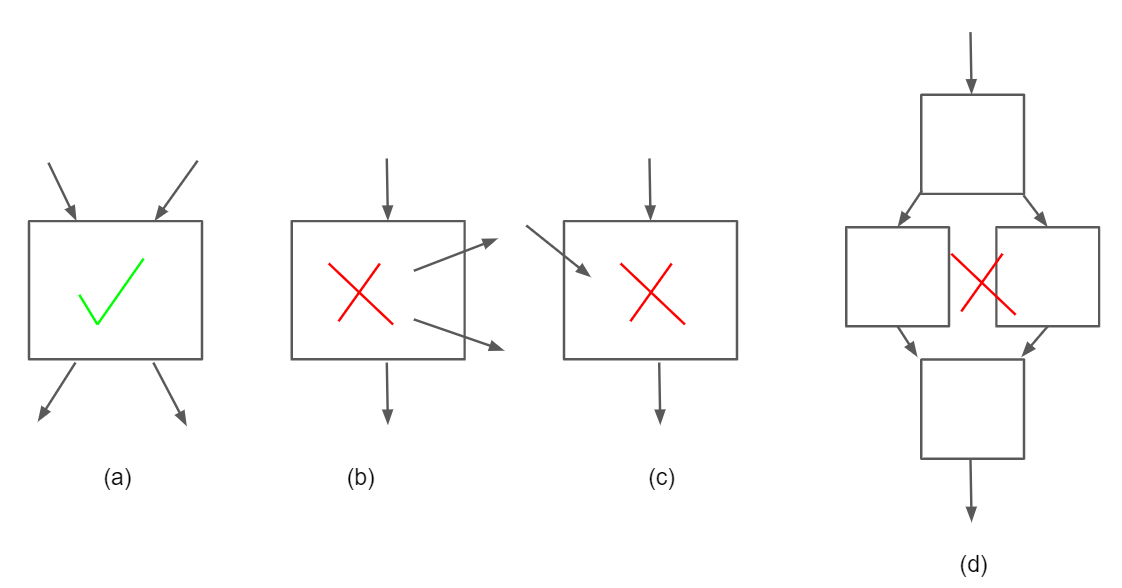
\includegraphics[height=6cm]{1.png}
\caption{Examples and Counterexamples for basic block}
\end{figure}

Consider the following example of a single basic block:

\begin{enumerate}
    \item L:
    \item \(t := 2 * x\)
    \item \(w := t + x\)
    \item if w \(>\) 3 goto L'
\end{enumerate}

\begin{itemize}
    \item Is it ok to change (3) to \(w := 3 * x\) ?
    It is ok. If addition of two numbers is more expensive as compared to multiplication of a number with a constant, the above change can be considered an optimization.
    \item Is it ok to change (4) to if x \(>\) 1 goto L' ? It is not ok. Because here x is a finite bounded integer and due to overflow, it is possible to have \(3 * x > 3\) and not x \(>\) 1.
    \item Is it ok to remove (2) ? Depends on whether variable t is used later in the code or not.
\end{itemize}

\subsection{Control Flow Graph}

A control flow graph is a directed graph with
\begin{itemize}
    \item basic blocks as nodes
    \item edge from block A to block B if the execution can pass from the last instruction in A to the first instruction in B, for example
    \begin{itemize}
        \item the last instruction in A is: jump Lb
        \item the last instruction in A is: if id1 = id2 then goto Lb
        \item execution can fall-through from block A to block B
    \end{itemize}
\end{itemize}

Consider the following example of a CFG:

\begin{figure}[htp]
\centering
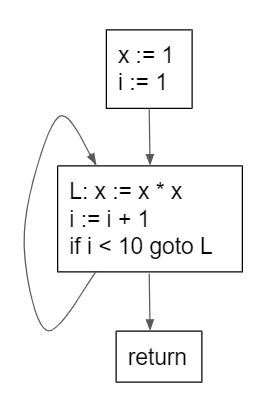
\includegraphics[height=6cm]{images/CFG Example.png}
\caption{CFG Example}
\end{figure}

The body of a method (or procedure) can be represented as a control-flow graph. There is one initial node (entry node). All "return" nodes are terminal.

\subsection{Optimization}
The optimizations are performed on the control flow graph of the intermediate representation of the code to improve program's resource utilization:

\begin{itemize}
    \item Execution Time
    \item Code Size
    \item Memory Usage
    \item Frequency of Disk I/O operations (or network operations)
    \item Power Consumption (Not same as energy)
\end{itemize}

It is important to remember that optimization should not alter the meaning of the program. It should not alter what the program computes.

For example, the following optimization changes the meaning of the program and thus, it is not a valid optimization.

w := 3 * x
if w \(>\) 3 goto L  

cannot be converted to: if x \(>\) 1 goto L

\subsection{Typical Granularity of Optimization}

\begin{enumerate}
    \item \textbf{Local Optimizations}
    \begin{itemize}
        \item applied to a basic block in isolation
        \item easiest to implement
    \end{itemize}
    
    \item \textbf{Global Optimizations}
    \begin{itemize}
        \item applied to a CFG (method body) in isolation while crossing the boundaries of basic blocks
    \end{itemize}
        
    \item \textbf{Inter-Procedural Optimizations}
    \begin{itemize}
        \item applied across method (CFG) boundaries
        \item difficult to implement but usually most effective
    \end{itemize}
\end{enumerate}

\subsection{Economics of the Optimization}

Optimizations are more of an art rather than science. The current state of the art methods are based on the concept of "Maximum benefit for minimum cost" where cost can denote the development and integration costs of the optimization.

\begin{itemize}
    \item Some optimizations are hard to implement
    \item Some optimizations require large compilation time
    \item Some optimizations have low payoff (the benefits) and it is often difficult to quantify payoff.
\end{itemize}

%\section{Local Optimizations}

Local Optimizations are the simplest form of optimizations that can be performed by considering a single basic block in isolation. Some possible examples are:

\begin{itemize}
    \item \textbf{Elimination of No-ops:} Some statements can be deleted. \(x := x + 0\), \(x := x * 1\), \(x := x | 0\)
    \item \textbf{Algebraic Simplification:} Some statements can be simplified
    \[x := x * 0 \rightarrow x := 0\]
    \[y := x ** 2 \rightarrow y := x * x\]
    \[x := x * 8 \rightarrow x := x << 3\]
    \[x := x * 15 \rightarrow t := x << 4; x := t - x\]
    
    The above code replacements are meaningful optimizations only if the RHS code would perform better than LHS code which also depends on the underlying hardware.
    \item \textbf{Constant Propagation or Constant Folding:} For statement x := y op z where y and z are constants, this statement can be computed at compile time.
    \[x := 2 + 2 \rightarrow x := 4\]
    \[if\; 2 < 0\; jump\; L \rightarrow No-op\]
    \[if\;2>0\;jump\;L \rightarrow jump\;L\]
    
    More specifically, constant folding is about performing computations at compile time and constant propagation is about propagating constants throughout the program.
\end{itemize}

\subsection{Dead Code Elimination}

Dead code is the code that is unreachable from the initial block, for example, CFG node with no incoming edges. Removing unreachable code makes the program smaller (and sometimes faster due to fewer cache misses).
\\
\\
\textbf{Why would unreachable block occur?}
\\
\#define DEBUG 0
\\
...
\\
if (DEBUG) \{
\\
...
\\
\}
\\

In the above example, after performing constant propagation, DEBUG would be replaced with 0. Further constant folding would remove the jump statement to the 'if' block and it would be converted to dead code which can be eliminated.

Unreachable block may also occur when libraries are imported. Libraries might have a large number of functions but usually only a small fraction of functions are actually used. Then the code for other functions constitute dead code. Usually other optimizations may result in more dead code.

\subsection{Common Subexpression Elimination}

Consider the case of following code with the assumption that the value of x, y, and z remain unchanged after the first statement, then we can perform the following replacement to use the pre-computed value.

x := y + z;
...;
...;
w := y + z; $\;\;\; \rightarrow \;\;\;$ x := y + z; ...; ...; w := x;

In this case, SSA IR particularly helps in doing away with the initial assumption since SSA IR enforces the property that each variable can be assigned only once. In short, SSA IR makes more values available simultaneously.

\[x_1 := y + z; x_2 := x_1 + 3; w := y + z \;\;\; \rightarrow \;\;\; x_1 := y + z; x_2 := x_1 + 3; w := x_1\]

In the above example, the common subexpression being eliminated is y + z. The three address code also makes it easier to identify the uses of a subexpression in the code.

\subsection{Copy Propagation}

If we see w := x, replace subsequent uses of w with x (and eliminate this statement)\\
\\
Before: x := y + z; w := x + 3; v := x; u := v + 3;\\
After: x := y + z; w := x + 3; u := x + 3;\\
\\
This optimization leads to less number of copies leading to need of fewer registers. It also activates further optimizations like common subexpression elimination.

\subsection{Example 1}

\textbf{Original Code:} x := y + z; w := x + 3; v := y + z; u := v + 3;\\
\textbf{After CSE:} x := y + z; w := x + 3; v := x; u := v + 3;\\
\textbf{After CP:} x := y + z; w := x + 3; u := x + 3;\\
\textbf{After CSE:} x := y + z; w := x + 3; u := w;\\
\\
Further copy propagation is possible due to the third statement u := w.

\subsection{Example 2}

a := x ** 2
b := 3\\
c := x\\
d := c * c\\
e := b * 2\\
f := a + d\\
g := e + f\\

\textbf{Final form: }

a := x * x
f := a + a
g := 6 * f\\
\\
It is possible for the compiler to get stuck in a "local minima". In the above example, if f := 2 * a was not replaced with f := a + a, there could have been possibility to use the shift operator (f := a \(<<\) 1) or to use copy propagation followed by dead code elimination (a:= x * x; g := 12 * a)

\subsection{Summary}
\begin{itemize}
    \item Each local optimization does little by itself.
    \item Often optimizations interact: performing one optimization may enable of disable other optimizations.
    \item Optimizing compilers can be thought of as a big bag of tricks.
\end{itemize}

\subsection{Typical Structure of an Optimizing Compiler}
repeat \{apply an optimization rule\}\\
until \{no improvement is possible\}

\begin{itemize}
    \item \textbf{Convergence} can be guaranteed by defining a metric for performance and ensuring that each iteration improves that metric. This monotonic behaviour would prevent any kind of oscillations that might be possible.
    \item \textbf{Optimality} is not guaranteed. The compiler can get stuck in a local minima.
\end{itemize}
 
%\section{Peephole Optimizations}

A peephole optimization is a type of local optimization based on a pattern matching rule consisting of a pattern and a replacement. Here, both pattern and replacement are templates for a sequence of instructions.

\[pattern \rightarrow replacement\]
\[i_1, i_2, ... , i_n \rightarrow j_1, j_2, ..., j_m\]

The main idea here is to scan the code and look for the code matching the pattern template and replace it with the replacement code which might be better than the original code in utilization of one of the program's resources. Traditionally the peephole optimization has been quite successfully used on assembly code.

Some examples of peephole optimizations are as follows:

\begin{itemize}
    \item move \$r1 \$r2; move \$r2, \$r1 $\rightarrow$ move \$r1 \$r2
    
    Possible to do the above replacement because after the first instruction, second move is just a nop and can be removed. It is equivalent to dead code elimination. Do note that the registers mentioned in the instructions are simply placeholders and there can be some other registers as well. 
    \item addiu \$r1, \$r1, i; addiu \$r1, \$r1, i $\rightarrow$ addiu \$r1, \$r1, i + j
    
    Again registers and constants in the above instructions are simple placeholders and can take any arbitrary value. The above example can be considered as constant folding cast as peephole optimization.
    \item addiu \$r1, \$r2, 0 $\rightarrow$ move \$r1, \$r2
    \item move \$r1 \$r1 $\rightarrow$ \(<\) empty \(>\)
\end{itemize}

The peephole optimizations are implemented as a database of rules. An optimizer, then scans the code to find the code that matches any pattern in the database and then can be replaced by the replacement.

Many (but not all) local optimizations can be cast as peephole optimizations. Some examples and counterexamples are as follows:

\begin{itemize}
    \item Algebraic simplification: If an instruction multiplies the value in a register with some power of 2, it can be replaced by a shift instruction.
    \item Copy Propagation: It cannot be cast as peephole optimization as the definition of a variable and its usage can be very far away with multiple instructions in between with various combinations making it difficult to match them to a pattern
    \[w := x\]
    \[...\]
    \[...\]
    \[t := w + 1\]
\end{itemize}

Like local optimizations, peephole optimizations can be applied repeatedly. Applying one peephole optimization can activate as well as curb other usages of peephole optimizations. Thus, peephole optimizations are used iteratively a fixed number of times or until no further patterns can be found.

The idea of peephole optimizations becomes more attractive if these can be generated automatically instead of manually coded. Use of enumerative and stochastic methods have been there to automatically learn peephole optimizations.

"Program optimization" is grossly misnamed. Present day "optimizers" have no intention or even pretense of working towards the optimal program. They work towards improving the performance of the code based on certain patterns. Therefore, code "improvers" is a better term.

\section{Global Optimizations} 
\setlength{\parindent}{0pt}

(Prepared by Aditya Senthilnathan)

\vspace{0.3cm}

Global optimisations go beyond the scope of a single basic block. It needs reasoning of the whole control flow graph which may be within the body of a method.

% Example 1
% Example 2

\subsection{Global Constant Propagation}

\begin{itemize}
    \item This is similar to local constant propagation but now we are reasoning in a global level (across several basic blocks within the body of a method)
    \item In this optimisation, we basically ask the question "When can we replace the use of a variable \textbf{x} with a constant \textbf{k}
    
    Ans: If on \textbf{every path} to the use of x, if the \textbf{last assignment} to x is \textbf{x:=k}, then we can do this transformation/optimisation.
\end{itemize}

% Example 3

The algorithm for global constant propagation requires a class of algorithms which are called "Global Dataflow Analysis". This kind of reasoning (with paths, etc.) is required for many different types of optimisation problems in compilers. And so, it helps to create a common framework in which we can implement the same logic but with different kinds of properties so that there is reuse of the same idea.

Let's identify some traits that global optimisations tasks share:

\begin{itemize}
    \item \underline{Optimisation depends on knowing property X at a certain program point P}
    
    Eg. In global constant propagation, we were interested in knowing if x:=k is the last assignment on all possible paths, at the program point of the last basic block (where x is used) in our example graph.
    
    \item \underline{Proving X at P requires knowledge of entire program}
    
    Eg. In our global constant propagation example, to be able to say x:=k is the last assignment to x on all possible paths that can reach program point P, we need to know the characteristics of the entire program. As opposed to local optimistaion where you only need info about the concerned basic block. Here, even though transformation is only made in a basic block, it relies on a property that requires knowledge of the entire program.
    
    \item \underline{It's OK to be conservative}
    
    We can either say,
    \begin{center}
        \textit{X is definitely true}
    \end{center}
    or say,
    \begin{center}
        \textit{We don't know if X is true}    
    \end{center}
    
    We want to get "X is definitely true" as much as possible because only then can we apply the transformation but if we get the conservative answer "We don't know if X is true", then we don't apply the transformation to preserve program correctness. Knowing if X is definitely not true is useless because in this case we still don't apply the transformation and so this use case is clubbed with "We don't know if X is true".
\end{itemize} 
\setlength{\parindent}{0pt}

\section{DFA Values}

(Prepared by Aditya Senthilnathan)

Recall that for global constant propagation, we need the following:

\vspace{0.3cm}

\underline{\textit{Optimisation}}: Replace a use of x by a constant k

\underline{\textit{Constraint}}: On every path to the use of x, the last assignment to x should be x:=k

\vspace{0.3cm}

We need to do this for every variable in the program. But first let's do this for a single variable x and then we can generalise it to more variables.

\subsection{Dataflow Analysis Values}

These are abstract values that are supposed to capture the set or category of concrete values that x (a variable) may take.

\vspace{0.5cm}

At each program point, we associate one of the following values with X (a variable),
\begin{center}
    \begin{tabular}{| m{2cm} | m{7cm} |}
        \hline
        Value & Explanation \\
        \hline
        $\top$ (top) &
        This value represents either that
        \begin{itemize} 
            \item This statement never executes
            \item or we have not executed or seen it yet
        \end{itemize}\\
        \hline
        $\bot$ (bottom) &
        This value represents either that
        \begin{itemize} 
            \item We can't say that X is a constant
            \item X is definitely not a constant
        \end{itemize}\\
        \hline
        $C$ (constant) &
        This value represents that X is a constant $C$\\
        \hline
    \end{tabular}
\end{center}

\vspace{0.5cm}

\textbf{Question:} \underline{What are we trying to do here? What do these values mean?}

\vspace{0.3cm}

\textbf{Answer:} We are trying to figure out what are the possible values of X (a variable) at every program point. The values we are talking about essentially tell us if the program reached here what is the value of X or all the possible values of X at this program point.

Now we will discuss each of the values in a little more detail,
\begin{itemize}
    \item \underline{$\top$ (top)} - This value represents that this statement never executes i.e the program/control never reaches here. This might be because this part of the program is never reachable from the beginning of the program. So in this case we just say that the value is $\top$ here because the statement never executes and therefore it is not meaningful to say what this value is.
    \item \underline{C (constant)} - It could be any constant. Eg. 0,1,2,-2,etc. This value says that whenever this program point is reached, irrespective of the path taken, we are sure that X will be equal to constant value C at this point.
    \item \underline{$\bot$ (bottom)} - This value essentially says that we don't know if X is a constant or not at this point. We are not sure of it's value. This might be happening because it's possible that on different paths X could take different values or on some path X is not a constant, etc. Even if we know for sure that X is not a constant, we still assign $\bot$ to X. This is a conservative assignment. Technically, even if we (DFA algorithm) assign $\bot$ to X at every program point conservatively, then this solution is also correct but it is trivially true and is not of much use to us.
\end{itemize}

\textbf{Note:} If we're still in the middle of execution of the DFA algorithm and at a particular point, we have value $\top$ for one of the variables in the program then it could also mean that the DFA algorithm hasn't seen this point yet or hasn't reached this point yet. The above discussion and interpretation of $\top$ only applies if a variable has $\top$ value after the DFA algorithm has finished executing

\subsection{Using DFA values for transformation}

Given global constant information ($\top$, $\bot$, C)
\begin{itemize}
    \item Inspect x = $?$ (either $\top$ or $\bot$ or C) at the program point that just precedes the statement which you want to examine (the statement that uses x)
    \item If x = C, then replace the use of x with C
\end{itemize}

For some examples of how to assign DFA values see the 
\href{https://www.youtube.com/watch?v=EI56VONzCcc&list=PLf3ZkSCyj1tf3rPAkOKY5hUzDrDoekAc7&index=75&ab_channel=compilerai}{lecture video}

\section{Dataflow Analysis Algorithm (DFA)}

(Prepared by Aditya Senthilnathan)

In this section, we will now try to answer the question "How do we identify what the DFA value should be at every program point?"

We will only analyse one particular variable x for now. This can easily be generalised for arbitrary number of variables and this is left to the reader.

\subsection{Insight}

DFA of a complex and large program can be expressed as a combination of simple rules relating the change in information between adjacent statements.

\vspace{0.3cm}

We're just going to see
\begin{itemize}
    \item What the value of x is just before this statement
    \item What is the current statement
    \item Based on the current statement, we then use rules (to be discussed) to compute what should be the value after the statement
\end{itemize}

One way to think about this is that we are "pushing" or "transferring" information from one statement to the next. It's almost just like program execution with the caveat that we are not dealing with concrete values anymore but rather abstract DFA values.

\subsection{Function for "Constant Information"}

We now define a function $C(x, s, in/out)$ where,

\begin{itemize}
    \item $x$ - variable for which we want to compute abstract values
    \item $s$ - statement s in the program
    \item $in/out$ - whether it is input to the statement or output to the statement i.e just before the statement or just after the statement.
    \begin{itemize}
        \item $C(x, s, in)$ = Value of x just before s
        \item $C(x, s, out)$ = Value of x just after s i.e just after statement s is executed
    \end{itemize}
\end{itemize}

The idea is to calculate the value of this function $C(x, s, in/out)$ for every x and every s (both in and out)

\subsection{Transfer Function}

We need to define how information is transferred from one statement to another i.e how are we pushing information. For this we need to define a transfer function.

\begin{center}
    \underline{Transfer Function:} transfers information from one statement to another
\end{center}

We are going to define rules for the following two cases:

\begin{itemize}
    \item \textbf{Case 1:} There are one or more predecessor points with edges to the current program point. In this case, we will see how to combine information/values flowing in from the predecessor points to assign a value for the $C()$ function in the current program point
    \item \textbf{Case 2:} For a given statement s, we see how the information/value is modified as it flows through the statement
\end{itemize}

\subsubsection{Transfer function for Global Constant Propagation}

We will define the function by doing an exhaustive case analysis. We can do this kind of finite description of the function with an exhaustive case analysis because there are only a limited number of values and cases to consider.

\vspace{0.3cm}

$C(x, s, p)$ can take only one of 3 different unique values during and after execution of the DFA algorithm i.e $\top, \bot, C$. Also once the algorithm picks a constant value for x at a particular program point, the constant value is fixed and it cannot vary after that. Eg. If the DFA algorithm picks 3, it cannot assign 4 later on. It can only change to either $\top$ or $\bot$ later on in the execution.

\vspace{0.3cm}

\textbf{Rules for the Transfer function:}

\begin{enumerate}
    \item If $C(x, p, out) = \bot$ then $\forall s \in$ successors(p), $C(x, s, in) = \bot$
    % Insert image
    \item If $C(x, s, in) = C$ and s does not modify x then, $C(x, s, out) = C$
    % Insert image
    \item If $C(p_i, x, out) = \bot$ for any i, then $C(x, s, in) = \bot$
    % Insert image
    \item If $C(p_i, x, out) = c$ and $C(p_j, x, out) = d$ and $c \neq d, i \neq j$ for some $i, j$ then, $C(s,x,in) = \bot$
    % Insert image
    \item If $C(p_i, x, out) = c$ or $C(p_i, x, out) = \top$ for all i, then $C(s, x, in) = c$
    \item If $C(p, x_i, out) = \top$ for all i, then $C(s, x, in) = \top$
    \item If $C(s, x, in) = \top$, then $C(s, x, out) = \top$
    \item If rule 7 does not apply i.e $C(s,x,in) \neq \top$, then $C(x := c, x, out) = c$ [where c is a constant]
    \item If rule 7 does not apply i.e $C(s,x,in) \neq \top$, then $C(x := f(...), x, out) = \bot$
    \item $C(y := ..., x, out) = C(y:=..., x, in)$ where $y \neq x$
\end{enumerate}

We now have 10 rules relating $C(s, x, in/out)$ to the value of this function at a predecessor point. These rules are exhaustive.

\vspace{0.3cm}

\underline{But so far we have just stated the rules. How do we get the actual values?}

\vspace{0.3cm}

Think of this as a system of equations. We are interested in solving and identifying values for this $C$ function such that all 10 rules are satisfied.

\vspace{0.3cm}

\underline{How do we solve this system of equations?}

\vspace{0.3cm}

Note that there is a trivial solution,

\begin{center}
    $C(s, x, in/out) = \bot$, for all statements s
\end{center}

All 10 rules are satisfied by this solution but this solution is useless to us because it doesn't allow us to perform any transformations/optimizations. We're not interested in just any solution. We are interested in the "most precise" solution (for some notion of precision). For eg. Saying that $x=4$ at some program point is more precise than just saying $x=\bot$. Similarly, saying that $x=\top$ is more precise than saying $x=\bot$ because the fact that this program point is unreachable is still useful information because now we can consider doing dead code elimination in this part of the program.

\vspace{0.3cm}

To solve this system of equations in a more precise way, we use a Fixed Point Iteration Algorithm.

\vspace{0.3cm}

\underline{Algorithm:}

\vspace{0.3cm}

\begin{itemize}
    \item At every entry point s to the program, set $C(s, x, in) = \bot$
    \item At every other statement s (which is non-entry), set $C(s,x,in) = \top$
    \item For every statement s, $C(s,x,out) = \top$
    \item Repeat the following until all program points satisfy rules 1-10:
    \begin{itemize}
        \item Pick a statement s not satisfying one or more rules in rules 1-10 and update the corresponding $C()$ function value using the appropriate rule
    \end{itemize}
\end{itemize}

There is a guarantee that this algorithm will converge. It will also give us the most precise answer. In the worst case, the solution it gives will be $\bot$ at all program points.

 

\definecolor {processblue}{cmyk}{0.96,0,0,0}
\clearpage

\section{DFA Example}
We will apply the fixed point algorithm to the variable ``x" in the following piece of code.


\begin{figure}[h!]
\caption{Example}
\begin {center}
\begin {tikzpicture}[-latex ,auto ,node distance =3.5cm and 5cm ,on grid ,
semithick ,
state/.style ={ rectangle ,top color =white , bottom color = processblue!20 ,
draw,processblue , text=blue , scale = 0.7 ,minimum width =3.5 cm, minimum height = 2.5 cm}]
\node[state] (A) node [label = {[label distance = 0.55cm]90:Block A}, rectangle split,rectangle split parts=2]{%
  x := 3
  \nodepart{second}
  b \textgreater  0?%
  };
\node[state] (B) [below left = of A] node [label = {[label distance = 0.55cm]90:Block B},rectangle split,rectangle split parts=2] [below left = of A] {%
  y := z + w
  \nodepart{second}
  x := 4%
  };
\node[state] (D) [below right =of A] node [label = {[label distance = 0.55cm]90:Block C},rectangle split,rectangle split parts=2] [below right = of A] {%
  y := 0
  \nodepart{second}
  %
  };
\node[state] (E) [below left =of D] node [label = {[label distance = 0.55cm]90:Block D},rectangle split,rectangle split parts=2] [below left = of D] {%
  a := 2 * x
  \nodepart{second}
  %
  };
\path[->] (A) edge node [align = center][above = 0.3 cm] {$false$} (D);
\path[->] (A) edge node [align = center][above = 0.3 cm] {$true$} (B);
\path[->] (B) edge node [align = center][above = 0.3 cm] {$$} (E);
\path[->] (D) edge node [align = center][above = 0.3 cm] {$$} (E);
\end{tikzpicture}
\end{center}
\end{figure}

\clearpage
Next figure shows all the program points in our example. Program points are all the points that appear before and after every statement. In case of only one predecessor, the ``out of the predecessor" is merged with the ``in of the successor" while working on this piece of code. ``---" marks the program points in the example we are working on.


\begin{figure}[h!]
\caption{Program Points}
\begin {center}
\begin {tikzpicture}[-latex ,auto ,node distance =3.5cm and 5cm ,on grid ,
semithick ,
state/.style ={ rectangle ,top color =white , bottom color = processblue!20 ,
draw,processblue , text=blue , scale = 0.7 ,minimum width =3.5 cm, minimum height = 3.5 cm}]
\node[state] (A) node [label = {[label distance = 0.3cm]90:Block A},rectangle split,rectangle split parts=5]{%
  ---
  \nodepart{second}
  x := 3
  \nodepart{third}
  ---
  \nodepart{fourth}
  b \textgreater 0? 
  \nodepart{five}
  ---%
  };
\node[state] (B) [below left = of A] node [label = {[label distance = 0.3cm]90:Block B}, rectangle split,rectangle split parts=5] [below left = of A] {%
  ---
  \nodepart{two}
  y := z + w
  \nodepart{three}
  ---
  \nodepart{four}
  x := 4
  \nodepart{five}
  ---%
  };
\node[state] (D) [below right =of A] node [label = {[label distance = 0.65cm]90:Block C}, rectangle split,rectangle split parts=3] [below right = of A] {%
  ---
  \nodepart{second}
  y := 0
  \nodepart{third}
  ---
  %
  };
\node[state] (E) [below left =of D] node [label = {[label distance = 0.65cm]90:Block D}, rectangle split,rectangle split parts=3] [below left = of D] {%
  ---
  \nodepart{two}
  a := 2 * x
  \nodepart{three}
  ---
  %
  };
\path[->] (A) edge node [align = center][above = 0.3 cm] {$false$} (D);
\path[->] (A) edge node [align = center][above = 0.3 cm] {$true$} (B);
\path[->] (B) edge node [align = center][above = 0.3 cm] {$$} (E);
\path[->] (D) edge node [align = center][above = 0.3 cm] {$$} (E);
\end{tikzpicture}
\end{center}
\end{figure}

\clearpage


Algorithm starts by initializing every value to $\top$(top) except the ``in of entry statement" which is initialized to $\bot$(bottom).

\begin{figure}[h!]
\caption{Initialization}
\begin {center}
\begin {tikzpicture}[-latex ,auto ,node distance =3.5cm and 5cm ,on grid ,
semithick ,
state/.style ={ rectangle ,top color =white , bottom color = processblue!20 ,
draw,processblue , text=blue , scale = 0.7 ,minimum width =3.5 cm, minimum height = 3.5 cm}]
\node[state] (A) node [label = {[label distance = 0.2cm]90:Block A}, rectangle split,rectangle split parts=5]{%
  $\bot$
  \nodepart{second}
  x := 3
  \nodepart{third}
  $\top$
  \nodepart{fourth}
  b \textgreater 0? 
  \nodepart{five}
  $\top$%
  };
\node[state] (B) [below left = of A] node [label = {[label distance = 0.2cm]90:Block B},rectangle split,rectangle split parts=5] [below left = of A] {%
  $\top$
  \nodepart{two}
  y := z + w
  \nodepart{three}
  $\top$
  \nodepart{four}
  x := 4
  \nodepart{five}
  $\top$%
  };
\node[state] (D) [below right =of A] node [label = {[label distance = 0.6cm]90:Block C},rectangle split,rectangle split parts=3] [below right = of A] {%
  $\top$
  \nodepart{second}
  y := 0
  \nodepart{third}
  $\top$
  %
  };
\node[state] (E) [below left =of D] node [label = {[label distance = 0.6cm]90:Block D},rectangle split,rectangle split parts=3] [below left = of D] {%
  $\top$
  \nodepart{two}
  a := 2 * x
  \nodepart{three}
  $\top$
  %
  };
\path[->] (A) edge node [align = center][above = 0.3 cm] {$false$} (D);
\path[->] (A) edge node [align = center][above = 0.3 cm] {$true$} (B);
\path[->] (B) edge node [align = center][above = 0.3 cm] {$$} (E);
\path[->] (D) edge node [align = center][above = 0.3 cm] {$$} (E);
\end{tikzpicture}
\end{center}
\end{figure}
\clearpage
Now the algorithm will pick the statement which does not follow the transfer function rules, which is the ``x := 3" statement in this example, and update it. The ``out of the statement" should be Constant 3 according to the transfer function rule. After updating the ``out of the statement", we get this graph.



\begin{figure}[h!]
\caption{``x := 3" statement update}
\begin {center}
\begin {tikzpicture}[-latex ,auto ,node distance =3.5cm and 5cm ,on grid ,
semithick ,
state/.style ={ rectangle ,top color =white , bottom color = processblue!20 ,
draw,processblue , text=blue , scale = 0.7 ,minimum width =3.5 cm, minimum height = 4 cm}]
\node[state] (A) node [label = {[label distance = 0.2cm]90:Block A}, rectangle split,rectangle split parts=5]{%
  $\bot$
  \nodepart{second}
  x := 3
  \nodepart{third}
  $C(3)$
  \nodepart{fourth}
  b \textgreater 0? 
  \nodepart{five}
  $\top$%
  };
\node[state] (B) [below left = of A] node [label = {[label distance = 0.2cm]90:Block B},rectangle split,rectangle split parts=5] [below left = of A] {%
  $\top$
  \nodepart{two}
  y := z + w
  \nodepart{three}
  $\top$
  \nodepart{four}
  x := 4
  \nodepart{five}
  $\top$%
  };
\node[state] (D) [below right =of A] node [label = {[label distance = 0.7cm]90:Block C},rectangle split,rectangle split parts=3] [below right = of A] {%
  $\top$
  \nodepart{second}
  y := 0
  \nodepart{third}
  $\top$
  %
  };
\node[state] (E) [below left =of D] node [label = {[label distance = 0.7cm]90:Block D},rectangle split,rectangle split parts=3] [below left = of D] {%
  $\top$
  \nodepart{two}
  a := 2 * x
  \nodepart{three}
  $\top$
  %
  };
\path[->] (A) edge node [align = center][above = 0.3 cm] {$false$} (D);
\path[->] (A) edge node [align = center][above = 0.3 cm] {$true$} (B);
\path[->] (B) edge node [align = center][above = 0.3 cm] {$$} (E);
\path[->] (D) edge node [align = center][above = 0.3 cm] {$$} (E);
\end{tikzpicture}
\end{center}
\end{figure}

\clearpage

The algorithm repeats this process until all program points satisfy the transfer function rules.


\begin{figure}[h!]
\caption{``b \textgreater 0?" statement update}
\begin {center}
\begin {tikzpicture}[-latex ,auto ,node distance =3.5cm and 5cm ,on grid ,
semithick ,
state/.style ={ rectangle ,top color =white , bottom color = processblue!20 ,
draw,processblue , text=blue , scale = 0.7 ,minimum width =3.5 cm, minimum height = 4 cm}]
\node[state] (A) node [label = {[label distance = 0.2cm]90:Block A},rectangle split,rectangle split parts=5]{%
  $\bot$
  \nodepart{second}
  x := 3
  \nodepart{third}
  $C(3)$
  \nodepart{fourth}
  b \textgreater 0? 
  \nodepart{five}
  $C(3)$%
  };
\node[state] (B) [below left = of A] node [label = {[label distance = 0.2cm]90:Block B},rectangle split,rectangle split parts=5] [below left = of A] {%
  $\top$
  \nodepart{two}
  y := z + w
  \nodepart{three}
  $\top$
  \nodepart{four}
  x := 4
  \nodepart{five}
  $\top$%
  };
\node[state] (D) [below right =of A] node [label = {[label distance = 0.7cm]90:Block C}, rectangle split,rectangle split parts=3] [below right = of A] {%
  $\top$
  \nodepart{second}
  y := 0
  \nodepart{third}
  $\top$
  %
  };
\node[state] (E) [below left =of D] node [label = {[label distance = 0.7cm]90:Block D}, rectangle split,rectangle split parts=3] [below left = of D] {%
  $\top$
  \nodepart{two}
  a := 2 * x
  \nodepart{three}
  $\top$
  %
  };
\path[->] (A) edge node [align = center][above = 0.3 cm] {$false$} (D);
\path[->] (A) edge node [align = center][above = 0.3 cm] {$true$} (B);
\path[->] (B) edge node [align = center][above = 0.3 cm] {$$} (E);
\path[->] (D) edge node [align = center][above = 0.3 cm] {$$} (E);
\end{tikzpicture}
\end{center}
\end{figure}

\clearpage

At this stage, there are two program points which do not satisfy the transfer function rules. The entry point of Block B and Block C do not match with their predecessors. We can update them.


\begin{figure}[h!]
\caption{``Successors of Block B and Block C" update}
\begin {center}
\begin {tikzpicture}[-latex ,auto ,node distance =3.5cm and 5cm ,on grid ,
semithick ,
state/.style ={ rectangle ,top color =white , bottom color = processblue!20 ,
draw,processblue , text=blue , scale = 0.7 ,minimum width =3.5 cm, minimum height = 4 cm}]
\node[state] (A) node [label = {[label distance = 0.2cm]90:Block A},rectangle split,rectangle split parts=5]{%
  $\bot$
  \nodepart{second}
  x := 3
  \nodepart{third}
  $C(3)$
  \nodepart{fourth}
  b \textgreater 0? 
  \nodepart{five}
  $C(3)$%
  };
\node[state] (B) [below left = of A] node [label = {[label distance = 0.2cm]90:Block B},rectangle split,rectangle split parts=5] [below left = of A] {%
  $C(3)$
  \nodepart{two}
  y := z + w
  \nodepart{three}
  $\top$
  \nodepart{four}
  x := 4
  \nodepart{five}
  $\top$%
  };
\node[state] (D) [below right =of A] node [label = {[label distance = 0.7cm]90:Block C}, rectangle split,rectangle split parts=3] [below right = of A] {%
  $C(3)$
  \nodepart{second}
  y := 0
  \nodepart{third}
  $\top$
  %
  };
\node[state] (E) [below left =of D] node [label = {[label distance = 0.7cm]90:Block D}, rectangle split,rectangle split parts=3] [below left = of D] {%
  $\top$
  \nodepart{two}
  a := 2 * x
  \nodepart{three}
  $\top$
  %
  };
\path[->] (A) edge node [align = center][above = 0.3 cm] {$false$} (D);
\path[->] (A) edge node [align = center][above = 0.3 cm] {$true$} (B);
\path[->] (B) edge node [align = center][above = 0.3 cm] {$$} (E);
\path[->] (D) edge node [align = center][above = 0.3 cm] {$$} (E);
\end{tikzpicture}
\end{center}
\end{figure}

\clearpage

Again there are two different statements that do not satisfy the transfer function rules, we can update them. 

\begin{figure}[h!]
\caption{``y := z + w" and ``y := 0" statements update}
\begin {center}
\begin {tikzpicture}[-latex ,auto ,node distance =3.5cm and 5cm ,on grid ,
semithick ,
state/.style ={ rectangle ,top color =white , bottom color = processblue!20 ,
draw,processblue , text=blue , scale = 0.7 ,minimum width =3.5 cm, minimum height = 4 cm}]
\node[state] (A) node [label = {[label distance = 0.2cm]90:Block A},rectangle split,rectangle split parts=5]{%
  $\bot$
  \nodepart{second}
  x := 3
  \nodepart{third}
  $C(3)$
  \nodepart{fourth}
  b \textgreater 0? 
  \nodepart{five}
  $C(3)$%
  };
\node[state] (B) [below left = of A] node [label = {[label distance = 0.2cm]90:Block B},rectangle split,rectangle split parts=5] [below left = of A] {%
  $C(3)$
  \nodepart{two}
  y := z + w
  \nodepart{three}
  $C(3)$
  \nodepart{four}
  x := 4
  \nodepart{five}
  $\top$%
  };
\node[state] (D) [below right =of A] node [label = {[label distance = 0.7cm]90:Block C}, rectangle split,rectangle split parts=3] [below right = of A] {%
  $C(3)$
  \nodepart{second}
  y := 0
  \nodepart{third}
  $C(3)$
  %
  };
\node[state] (E) [below left =of D] node [label = {[label distance = 0.7cm]90:Block D}, rectangle split,rectangle split parts=3] [below left = of D] {%
  $\top$
  \nodepart{two}
  a := 2 * x
  \nodepart{three}
  $\top$
  %
  };
\path[->] (A) edge node [align = center][above = 0.3 cm] {$false$} (D);
\path[->] (A) edge node [align = center][above = 0.3 cm] {$true$} (B);
\path[->] (B) edge node [align = center][above = 0.3 cm] {$$} (E);
\path[->] (D) edge node [align = center][above = 0.3 cm] {$$} (E);
\end{tikzpicture}
\end{center}
\end{figure}


\clearpage

At this stage, we can either update ``x := 4" statement, or we can update the successor of Block D. Irrespective of which one we pick, algorithm will return the same answer. In this example, we will update the successor of Block D. One predecessor is a constant, and other predecessor of Block D is $\top$. Using the 3rd transfer function rule, we can update the value of successor to the same constant.


\begin{figure}[h!]
\caption{``Successor of Block D" update}
\begin {center}
\begin {tikzpicture}[-latex ,auto ,node distance =3.5cm and 5cm ,on grid ,
semithick ,
state/.style ={ rectangle ,top color =white , bottom color = processblue!20 ,
draw,processblue , text=blue , scale = 0.7 ,minimum width =3.5 cm, minimum height = 4 cm}]
\node[state] (A) node [label = {[label distance = 0.2cm]90:Block A},rectangle split,rectangle split parts=5]{%
  $\bot$
  \nodepart{second}
  x := 3
  \nodepart{third}
  $C(3)$
  \nodepart{fourth}
  b \textgreater 0? 
  \nodepart{five}
  $C(3)$%
  };
\node[state] (B) [below left = of A] node [label = {[label distance = 0.2cm]90:Block B},rectangle split,rectangle split parts=5] [below left = of A] {%
  $C(3)$
  \nodepart{two}
  y := z + w
  \nodepart{three}
  $C(3)$
  \nodepart{four}
  x := 4
  \nodepart{five}
  $\top$%
  };
\node[state] (D) [below right =of A] node [label = {[label distance = 0.7cm]90:Block C}, rectangle split,rectangle split parts=3] [below right = of A] {%
  $C(3)$
  \nodepart{second}
  y := 0
  \nodepart{third}
  $C(3)$
  %
  };
\node[state] (E) [below left =of D] node [label = {[label distance = 0.7cm]90:Block D}, rectangle split,rectangle split parts=3] [below left = of D] {%
  $C(3)$
  \nodepart{two}
  a := 2 * x
  \nodepart{three}
  $\top$
  %
  };
\path[->] (A) edge node [align = center][above = 0.3 cm] {$false$} (D);
\path[->] (A) edge node [align = center][above = 0.3 cm] {$true$} (B);
\path[->] (B) edge node [align = center][above = 0.3 cm] {$$} (E);
\path[->] (D) edge node [align = center][above = 0.3 cm] {$$} (E);
\end{tikzpicture}
\end{center}
\end{figure}

\clearpage
Updating ``a := 2 * x" statement in Block D.

\begin{figure}[h!]
\caption{``a := 2 * x" update}
\begin {center}
\begin {tikzpicture}[-latex ,auto ,node distance =3.5cm and 5cm ,on grid ,
semithick ,
state/.style ={ rectangle ,top color =white , bottom color = processblue!20 ,
draw,processblue , text=blue , scale = 0.7 ,minimum width =3.5 cm, minimum height = 4 cm}]
\node[state] (A) node [label = {[label distance = 0.2cm]90:Block A},rectangle split,rectangle split parts=5]{%
  $\bot$
  \nodepart{second}
  x := 3
  \nodepart{third}
  $C(3)$
  \nodepart{fourth}
  b \textgreater 0? 
  \nodepart{five}
  $C(3)$%
  };
\node[state] (B) [below left = of A] node [label = {[label distance = 0.2cm]90:Block B},rectangle split,rectangle split parts=5] [below left = of A] {%
  $C(3)$
  \nodepart{two}
  y := z + w
  \nodepart{three}
  $C(3)$
  \nodepart{four}
  x := 4
  \nodepart{five}
  $\top$%
  };
\node[state] (D) [below right =of A] node [label = {[label distance = 0.7cm]90:Block C}, rectangle split,rectangle split parts=3] [below right = of A] {%
  $C(3)$
  \nodepart{second}
  y := 0
  \nodepart{third}
  $C(3)$
  %
  };
\node[state] (E) [below left =of D] node [label = {[label distance = 0.7cm]90:Block D}, rectangle split,rectangle split parts=3] [below left = of D] {%
  $C(3)$
  \nodepart{two}
  a := 2 * x
  \nodepart{three}
  $C(3)$
  %
  };
\path[->] (A) edge node [align = center][above = 0.3 cm] {$false$} (D);
\path[->] (A) edge node [align = center][above = 0.3 cm] {$true$} (B);
\path[->] (B) edge node [align = center][above = 0.3 cm] {$$} (E);
\path[->] (D) edge node [align = center][above = 0.3 cm] {$$} (E);
\end{tikzpicture}
\end{center}
\end{figure}

\clearpage

There is only one statement, ``x:=4" in Block B, that does not satisfy the transfer function rules. After updating it, we get this graph.

\begin{figure}[h!]
\caption{``x := 4" statement update}
\begin {center}
\begin {tikzpicture}[-latex ,auto ,node distance =3.5cm and 5cm ,on grid ,
semithick ,
state/.style ={ rectangle ,top color =white , bottom color = processblue!20 ,
draw,processblue , text=blue , scale = 0.7 ,minimum width =3.5 cm, minimum height = 4 cm}]
\node[state] (A) node [label = {[label distance = 0.2cm]90:Block A},rectangle split,rectangle split parts=5]{%
  $\bot$
  \nodepart{second}
  x := 3
  \nodepart{third}
  $C(3)$
  \nodepart{fourth}
  b \textgreater 0? 
  \nodepart{five}
  $C(3)$%
  };
\node[state] (B) [below left = of A] node [label = {[label distance = 0.2cm]90:Block B},rectangle split,rectangle split parts=5] [below left = of A] {%
  $C(3)$
  \nodepart{two}
  y := z + w
  \nodepart{three}
  $C(3)$
  \nodepart{four}
  x := 4
  \nodepart{five}
  $C(4)$%
  };
\node[state] (D) [below right =of A] node [label = {[label distance = 0.7cm]90:Block C}, rectangle split,rectangle split parts=3] [below right = of A] {%
  $C(3)$
  \nodepart{second}
  y := 0
  \nodepart{third}
  $C(3)$
  %
  };
\node[state] (E) [below left =of D] node [label = {[label distance = 0.7cm]90:Block D}, rectangle split,rectangle split parts=3] [below left = of D] {%
  $C(3)$
  \nodepart{two}
  a := 2 * x
  \nodepart{three}
  $C(3)$
  %
  };
\path[->] (A) edge node [align = center][above = 0.3 cm] {$false$} (D);
\path[->] (A) edge node [align = center][above = 0.3 cm] {$true$} (B);
\path[->] (B) edge node [align = center][above = 0.3 cm] {$$} (E);
\path[->] (D) edge node [align = center][above = 0.3 cm] {$$} (E);
\end{tikzpicture}
\end{center}
\end{figure}


\clearpage

Because of the previous update, the successor of the Block D does not satisfy the transfer function rules. According to the 2nd transfer function rule, it should have the value $\bot$.


\begin{figure}[h!]
\caption{``Successor of Block D" update}
\begin {center}
\begin {tikzpicture}[-latex ,auto ,node distance =3.5cm and 5cm ,on grid ,
semithick ,
state/.style ={ rectangle ,top color =white , bottom color = processblue!20 ,
draw,processblue , text=blue , scale = 0.7 ,minimum width =3.5 cm, minimum height = 4 cm}]
\node[state] (A) node [label = {[label distance = 0.2cm]90:Block A},rectangle split,rectangle split parts=5]{%
  $\bot$
  \nodepart{second}
  x := 3
  \nodepart{third}
  $C(3)$
  \nodepart{fourth}
  b \textgreater 0? 
  \nodepart{five}
  $C(3)$%
  };
\node[state] (B) [below left = of A] node [label = {[label distance = 0.2cm]90:Block B},rectangle split,rectangle split parts=5] [below left = of A] {%
  $C(3)$
  \nodepart{two}
  y := z + w
  \nodepart{three}
  $C(3)$
  \nodepart{four}
  x := 4
  \nodepart{five}
  $C(4)$%
  };
\node[state] (D) [below right =of A] node [label = {[label distance = 0.7cm]90:Block C}, rectangle split,rectangle split parts=3] [below right = of A] {%
  $C(3)$
  \nodepart{second}
  y := 0
  \nodepart{third}
  $C(3)$
  %
  };
\node[state] (E) [below left =of D] node [label = {[label distance = 0.7cm]90:Block D}, rectangle split,rectangle split parts=3] [below left = of D] {%
  $\bot$
  \nodepart{two}
  a := 2 * x
  \nodepart{three}
  $C(3)$
  %
  };
\path[->] (A) edge node [align = center][above = 0.3 cm] {$false$} (D);
\path[->] (A) edge node [align = center][above = 0.3 cm] {$true$} (B);
\path[->] (B) edge node [align = center][above = 0.3 cm] {$$} (E);
\path[->] (D) edge node [align = center][above = 0.3 cm] {$$} (E);
\end{tikzpicture}
\end{center}
\end{figure}

\clearpage

Updating the ``a = 2 * x" statement in Block D, we get this graph.


\begin{figure}[h!]
\caption{``a := 2 * x" statement update}
\begin {center}
\begin {tikzpicture}[-latex ,auto ,node distance =3.5cm and 5cm ,on grid ,
semithick ,
state/.style ={ rectangle ,top color =white , bottom color = processblue!20 ,
draw,processblue , text=blue , scale = 0.7 ,minimum width =3.5 cm, minimum height = 4 cm}]
\node[state] (A) node [label = {[label distance = 0.2cm]90:Block A},rectangle split,rectangle split parts=5]{%
  $\bot$
  \nodepart{second}
  x := 3
  \nodepart{third}
  $C(3)$
  \nodepart{fourth}
  b \textgreater 0? 
  \nodepart{five}
  $C(3)$%
  };
\node[state] (B) [below left = of A] node [label = {[label distance = 0.2cm]90:Block B},rectangle split,rectangle split parts=5] [below left = of A] {%
  $C(3)$
  \nodepart{two}
  y := z + w
  \nodepart{three}
  $C(3)$
  \nodepart{four}
  x := 4
  \nodepart{five}
  $C(4)$%
  };
\node[state] (D) [below right =of A] node [label = {[label distance = 0.7cm]90:Block C}, rectangle split,rectangle split parts=3] [below right = of A] {%
  $C(3)$
  \nodepart{second}
  y := 0
  \nodepart{third}
  $C(3)$
  %
  };
\node[state] (E) [below left =of D] node [label = {[label distance = 0.7cm]90:Block D}, rectangle split,rectangle split parts=3] [below left = of D] {%
  $\bot$
  \nodepart{two}
  a := 2 * x
  \nodepart{three}
  $\bot$
  %
  };
\path[->] (A) edge node [align = center][above = 0.3 cm] {$false$} (D);
\path[->] (A) edge node [align = center][above = 0.3 cm] {$true$} (B);
\path[->] (B) edge node [align = center][above = 0.3 cm] {$$} (E);
\path[->] (D) edge node [align = center][above = 0.3 cm] {$$} (E);
\end{tikzpicture}
\end{center}
\end{figure}


At this stage, there is no program point that violates any of the 8 transfer function rules, so the algorithm terminates by returning this \textbf{Fixed point solution} to us.

\subsection{Some Guarantees}
\begin{itemize}
    \item The fixed point solution will satisfy all the transfer function rules at each program point.
    \item The algorithm is guaranteed to converge, irrespective of whether the program has loops or not.
    \item Whenever there are multiple options to choose for a statement S to be updated, irrespective of which one we choose, we always get the same answer.
    \item The fixed point solution is going to have some precision guarantee, by some definition of precision, for the system of equations we are trying to solve.
\end{itemize}
 
\definecolor {processblue}{cmyk}{0.96,0,0,0}
\clearpage

\section{DFA Loop Example}

In this section, we will look at an example of DFA for a program with loops. We will apply the DFA algorithm on the variable ``x" in the following piece of code.

\begin{figure}[h!]
\caption{Example}
\begin {center}
\begin {tikzpicture}[-latex ,auto ,node distance =3.5cm and 5cm ,on grid ,
semithick ,
state/.style ={ rectangle ,top color =white , bottom color = processblue!20 ,
draw,processblue , text=blue , scale = 0.7 ,minimum width =3.5 cm, minimum height = 2.5 cm}]
\node[state] (A) node [label = {[label distance = 0.55cm]90:Block A}, rectangle split,rectangle split parts=2]{%
  x := 3
  \nodepart{second}
  b \textgreater  0?%
  };
\node[state] (B) [below left = of A] node [label = {[label distance = 0.55cm]90:Block B},rectangle split,rectangle split parts=2] [below left = of A] {%
  y := z + w
  \nodepart{second}
  x := 4%
  };
\node[state] (D) [below right =of A] node [label = {[label distance = 0.55cm]90:Block C},rectangle split,rectangle split parts=2] [below right = of A] {%
  y := 0
  \nodepart{second}
  %
  };
\node[state] (E) [below left =of D] node [label = {[label distance = 0.55cm]90:Block D},rectangle split,rectangle split parts=2] [below left = of D] {%
  a := 2 * x
  \nodepart{second}
  c == 0 ?
  %
  };
\path[->] (A) edge node [align = center][above = 0.3 cm] {$false$} (D);
\path[->] (A) edge node [align = center][above = 0.3 cm] {$true$} (B);
\path[->] (B) edge node [align = center][above = 0.3 cm] {$$} (E);
\path[->] (D) edge node [align = center][above = 0.3 cm] {$$} (E);
\path[->] (E) edge[bend right = 80] node [align = center][above = 0.3 cm] {$false$} (D);
\draw[->] (E) --++(0,-2.5cm) node[align = centre] [above left = 0.05cm] {$true$};

\end{tikzpicture}
\end{center}
\end{figure}



\clearpage
Next figure shows all the program points in our example. Program points are all the points that appear before and after every statement. In case of only one predecessor, the ``out of the predecessor" is merged with the ``in of the successor" while working on this piece of code. ``---" marks the program points in the example we are working on.


\begin{figure}[h!]
\caption{Program Points}
\begin {center}
\begin {tikzpicture}[-latex ,auto ,node distance =3.5cm and 5cm ,on grid ,
semithick ,
state/.style ={ rectangle ,top color =white , bottom color = processblue!20 ,
draw,processblue , text=blue , scale = 0.7 ,minimum width =3.5 cm, minimum height = 4 cm}]
\node[state] (A) node [label = {[label distance = 0.3cm]90:Block A},rectangle split,rectangle split parts=5]{%
  ---
  \nodepart{second}
  x := 3
  \nodepart{third}
  ---
  \nodepart{fourth}
  b \textgreater 0? 
  \nodepart{five}
  ---%
  };
\node[state] (B) [below left = of A] node [label = {[label distance = 0.3cm]90:Block B}, rectangle split,rectangle split parts=5] [below left = of A] {%
  ---
  \nodepart{two}
  y := z + w
  \nodepart{three}
  ---
  \nodepart{four}
  x := 4
  \nodepart{five}
  ---%
  };
\node[state] (D) [below right =of A] node [label = {[label distance = 0.65cm]90:Block C}, rectangle split,rectangle split parts=3] [below right = of A] {%
  ---
  \nodepart{second}
  y := 0
  \nodepart{third}
  ---
  %
  };
\node[state] (E) [below left =of D] node [label = {[label distance = 0.3cm]90:Block D}, rectangle split,rectangle split parts=5] [below left = of D] {%
  ---
  \nodepart{two}
  a := 2 * x
  \nodepart{three}
  ---
  \nodepart{four}
  c == 0?
  \nodepart{five}
  ---
  %
  };
\path[->] (A) edge node [align = center][above = 0.3 cm] {$false$} (D);
\path[->] (A) edge node [align = center][above = 0.3 cm] {$true$} (B);
\path[->] (B) edge node [align = center][above = 0.3 cm] {$$} (E);
\path[->] (D) edge node [align = center][above = 0.3 cm] {$$} (E);
\path[->] (E) edge[bend right = 80] node [align = center][above = 0.3 cm] {$false$} (D);
\draw[->] (E) --++(0,-2.5cm) node[align = centre] [above left = 0.05cm] {$true$};

\end{tikzpicture}
\end{center}
\end{figure}

\clearpage

Next step is to initialize all the program points. To do that, we initialize all the program points to value $\top$ except the entry points of the program which are initialized to $\bot$


\begin{figure}[h!]
\caption{Initialization}
\begin {center}
\begin {tikzpicture}[-latex ,auto ,node distance =3.5cm and 5cm ,on grid ,
semithick ,
state/.style ={ rectangle ,top color =white , bottom color = processblue!20 ,
draw,processblue , text=blue , scale = 0.7 ,minimum width =3.5 cm, minimum height = 4 cm}]
\node[state] (A) node [label = {[label distance = 0.3cm]90:Block A},rectangle split,rectangle split parts=5]{%
  $\bot$
  \nodepart{second}
  x := 3
  \nodepart{third}
  $\top$
  \nodepart{fourth}
  b \textgreater 0? 
  \nodepart{five}
  $\top$ %
  };
\node[state] (B) [below left = of A] node [label = {[label distance = 0.3cm]90:Block B}, rectangle split,rectangle split parts=5] [below left = of A] {%
  $\top$
  \nodepart{two}
  y := z + w
  \nodepart{three}
  $\top$
  \nodepart{four}
  x := 4
  \nodepart{five}
  $\top$ %
  };
\node[state] (D) [below right =of A] node [label = {[label distance = 0.65cm]90:Block C}, rectangle split,rectangle split parts=3] [below right = of A] {%
  $\top$
  \nodepart{second}
  y := 0
  \nodepart{third}
  $\top$
  %
  };
\node[state] (E) [below left =of D] node [label = {[label distance = 0.3cm]90:Block D}, rectangle split,rectangle split parts=5] [below left = of D] {%
  $\top$
  \nodepart{two}
  a := 2 * x
  \nodepart{three}
  $\top$
  \nodepart{four}
  c == 0?
  \nodepart{five}
  $\top$
  %
  };
\path[->] (A) edge node [align = center][above = 0.3 cm] {$false$} (D);
\path[->] (A) edge node [align = center][above = 0.3 cm] {$true$} (B);
\path[->] (B) edge node [align = center][above = 0.3 cm] {$$} (E);
\path[->] (D) edge node [align = center][above = 0.3 cm] {$$} (E);
\path[->] (E) edge[bend right = 80] node [align = center][above = 0.3 cm] {$false$} (D);
\draw[->] (E) --++(0,-2.5cm) node[align = centre] [above left = 0.05cm] {$true$};

\end{tikzpicture}
\end{center}
\end{figure}


\clearpage
In the next step, we identify the statements which do not follow the transfer function rules and start updating them. At this stage, only the statement ``x := 3" does not follow the transfer function rule, so we update it.

\begin{figure}[h!]
\caption{``x := 3" statement update}
\begin {center}
\begin {tikzpicture}[-latex ,auto ,node distance =3.5cm and 5cm ,on grid ,
semithick ,
state/.style ={ rectangle ,top color =white , bottom color = processblue!20 ,
draw,processblue , text=blue , scale = 0.7 ,minimum width =3.5 cm, minimum height = 4 cm}]
\node[state] (A) node [label = {[label distance = 0.3cm]90:Block A},rectangle split,rectangle split parts=5]{%
  $\bot$
  \nodepart{second}
  x := 3
  \nodepart{third}
  $C(3)$
  \nodepart{fourth}
  b \textgreater 0? 
  \nodepart{five}
  $\top$ %
  };
\node[state] (B) [below left = of A] node [label = {[label distance = 0.3cm]90:Block B}, rectangle split,rectangle split parts=5] [below left = of A] {%
  $\top$
  \nodepart{two}
  y := z + w
  \nodepart{three}
  $\top$
  \nodepart{four}
  x := 4
  \nodepart{five}
  $\top$ %
  };
\node[state] (D) [below right =of A] node [label = {[label distance = 0.65cm]90:Block C}, rectangle split,rectangle split parts=3] [below right = of A] {%
  $\top$
  \nodepart{second}
  y := 0
  \nodepart{third}
  $\top$
  %
  };
\node[state] (E) [below left =of D] node [label = {[label distance = 0.3cm]90:Block D}, rectangle split,rectangle split parts=5] [below left = of D] {%
  $\top$
  \nodepart{two}
  a := 2 * x
  \nodepart{three}
  $\top$
  \nodepart{four}
  c == 0?
  \nodepart{five}
  $\top$
  %
  };
\path[->] (A) edge node [align = center][above = 0.3 cm] {$false$} (D);
\path[->] (A) edge node [align = center][above = 0.3 cm] {$true$} (B);
\path[->] (B) edge node [align = center][above = 0.3 cm] {$$} (E);
\path[->] (D) edge node [align = center][above = 0.3 cm] {$$} (E);
\path[->] (E) edge[bend right = 80] node [align = center][above = 0.3 cm] {$false$} (D);
\draw[->] (E) --++(0,-2.5cm) node[align = centre] [above left = 0.05cm] {$true$};

\end{tikzpicture}
\end{center}
\end{figure}


\clearpage
The process of identifying the statement that violates the transfer function rules and updating it, is repeated until every program point satisfies them. At this stage, the ``b \textgreater 0?" statement violates the transfer function rules, so we update it.

\begin{figure}[h!]
\caption{``b \textgreater 0?" statement update}
\begin {center}
\begin {tikzpicture}[-latex ,auto ,node distance =3.5cm and 5cm ,on grid ,
semithick ,
state/.style ={ rectangle ,top color =white , bottom color = processblue!20 ,
draw,processblue , text=blue , scale = 0.7 ,minimum width =4 cm, minimum height = 4 cm}]
\node[state] (A) node [label = {[label distance = 0.3cm]90:Block A},rectangle split,rectangle split parts=5]{%
  $\bot$
  \nodepart{second}
  x := 3
  \nodepart{third}
  $C(3)$
  \nodepart{fourth}
  b \textgreater 0? 
  \nodepart{five}
  $C(3)$ %
  };
\node[state] (B) [below left = of A] node [label = {[label distance = 0.3cm]90:Block B}, rectangle split,rectangle split parts=5] [below left = of A] {%
  $\top$
  \nodepart{two}
  y := z + w
  \nodepart{three}
  $\top$
  \nodepart{four}
  x := 4
  \nodepart{five}
  $\top$ %
  };
\node[state] (D) [below right =of A] node [label = {[label distance = 0.65cm]90:Block C}, rectangle split,rectangle split parts=3] [below right = of A] {%
  $\top$
  \nodepart{second}
  y := 0
  \nodepart{third}
  $\top$
  %
  };
\node[state] (E) [below left =of D] node [label = {[label distance = 0.3cm]90:Block D}, rectangle split,rectangle split parts=5] [below left = of D] {%
  $\top$
  \nodepart{two}
  a := 2 * x
  \nodepart{three}
  $\top$
  \nodepart{four}
  c == 0?
  \nodepart{five}
  $\top$
  %
  };
\path[->] (A) edge node [align = center][above = 0.3 cm] {$false$} (D);
\path[->] (A) edge node [align = center][above = 0.3 cm] {$true$} (B);
\path[->] (B) edge node [align = center][above = 0.3 cm] {$$} (E);
\path[->] (D) edge node [align = center][above = 0.3 cm] {$$} (E);
\path[->] (E) edge[bend right = 80] node [align = center][above = 0.3 cm] {$false$} (D);
\draw[->] (E) --++(0,-2.5cm) node[align = centre] [above left = 0.05cm] {$true$};

\end{tikzpicture}
\end{center}
\end{figure}

\clearpage
At this stage, the successors of Block B and Block C do not satisfy the transfer function rules, so we can update them.



\begin{figure}[h!]
\caption{``Successors of Block B and Block C" update}
\begin {center}
\begin {tikzpicture}[-latex ,auto ,node distance =3.5cm and 5cm ,on grid ,
semithick ,
state/.style ={ rectangle ,top color =white , bottom color = processblue!20 ,
draw,processblue , text=blue , scale = 0.7 ,minimum width =4 cm, minimum height = 4 cm}]
\node[state] (A) node [label = {[label distance = 0.3cm]90:Block A},rectangle split,rectangle split parts=5]{%
  $\bot$
  \nodepart{second}
  x := 3
  \nodepart{third}
  $C(3)$
  \nodepart{fourth}
  b \textgreater 0? 
  \nodepart{five}
  $C(3)$ %
  };
\node[state] (B) [below left = of A] node [label = {[label distance = 0.3cm]90:Block B}, rectangle split,rectangle split parts=5] [below left = of A] {%
  $C(3)$
  \nodepart{two}
  y := z + w
  \nodepart{three}
  $\top$
  \nodepart{four}
  x := 4
  \nodepart{five}
  $\top$ %
  };
\node[state] (D) [below right =of A] node [label = {[label distance = 0.65cm]90:Block C}, rectangle split,rectangle split parts=3] [below right = of A] {%
  $C(3)$
  \nodepart{second}
  y := 0
  \nodepart{third}
  $\top$
  %
  };
\node[state] (E) [below left =of D] node [label = {[label distance = 0.3cm]90:Block D}, rectangle split,rectangle split parts=5] [below left = of D] {%
  $\top$
  \nodepart{two}
  a := 2 * x
  \nodepart{three}
  $\top$
  \nodepart{four}
  c == 0?
  \nodepart{five}
  $\top$
  %
  };
\path[->] (A) edge node [align = center][above = 0.3 cm] {$false$} (D);
\path[->] (A) edge node [align = center][above = 0.3 cm] {$true$} (B);
\path[->] (B) edge node [align = center][above = 0.3 cm] {$$} (E);
\path[->] (D) edge node [align = center][above = 0.3 cm] {$$} (E);
\path[->] (E) edge[bend right = 80] node [align = center][above = 0.3 cm] {$false$} (D);
\draw[->] (E) --++(0,-2.5cm) node[align = centre] [above left = 0.05cm] {$true$};

\end{tikzpicture}
\end{center}
\end{figure}


\clearpage

There are again two different statements ``y := z + w" and ``y:=0" that violate the transfer function rules, and we will update them.

\begin{figure}[h!]
\caption{``y := z + w" and "y := 0" statements update}
\begin {center}
\begin {tikzpicture}[-latex ,auto ,node distance =3.5cm and 5cm ,on grid ,
semithick ,
state/.style ={ rectangle ,top color =white , bottom color = processblue!20 ,
draw,processblue , text=blue , scale = 0.7 ,minimum width =4 cm, minimum height = 4 cm}]
\node[state] (A) node [label = {[label distance = 0.3cm]90:Block A},rectangle split,rectangle split parts=5]{%
  $\bot$
  \nodepart{second}
  x := 3
  \nodepart{third}
  $C(3)$
  \nodepart{fourth}
  b \textgreater 0? 
  \nodepart{five}
  $C(3)$ %
  };
\node[state] (B) [below left = of A] node [label = {[label distance = 0.3cm]90:Block B}, rectangle split,rectangle split parts=5] [below left = of A] {%
  $C(3)$
  \nodepart{two}
  y := z + w
  \nodepart{three}
  $C(3)$
  \nodepart{four}
  x := 4
  \nodepart{five}
  $\top$ %
  };
\node[state] (D) [below right =of A] node [label = {[label distance = 0.65cm]90:Block C}, rectangle split,rectangle split parts=3] [below right = of A] {%
  $C(3)$
  \nodepart{second}
  y := 0
  \nodepart{third}
  $C(3)$
  %
  };
\node[state] (E) [below left =of D] node [label = {[label distance = 0.3cm]90:Block D}, rectangle split,rectangle split parts=5] [below left = of D] {%
  $\top$
  \nodepart{two}
  a := 2 * x
  \nodepart{three}
  $\top$
  \nodepart{four}
  c == 0?
  \nodepart{five}
  $\top$
  %
  };
\path[->] (A) edge node [align = center][above = 0.3 cm] {$false$} (D);
\path[->] (A) edge node [align = center][above = 0.3 cm] {$true$} (B);
\path[->] (B) edge node [align = center][above = 0.3 cm] {$$} (E);
\path[->] (D) edge node [align = center][above = 0.3 cm] {$$} (E);
\path[->] (E) edge[bend right = 80] node [align = center][above = 0.3 cm] {$false$} (D);
\draw[->] (E) --++(0,-2.5cm) node[align = centre] [above left = 0.05cm] {$true$};

\end{tikzpicture}
\end{center}
\end{figure}

\clearpage

We have again two different statements that we can update at this stage, and we can choose to update anyone that we like, since the algorithm is guaranteed to return the same solution. In this example, we will update the ``x := 4" statement.

\begin{figure}[h!]
\caption{``x := 4" statement update}
\begin {center}
\begin {tikzpicture}[-latex ,auto ,node distance =3.5cm and 5cm ,on grid ,
semithick ,
state/.style ={ rectangle ,top color =white , bottom color = processblue!20 ,
draw,processblue , text=blue , scale = 0.7 ,minimum width =4 cm, minimum height = 4 cm}]
\node[state] (A) node [label = {[label distance = 0.3cm]90:Block A},rectangle split,rectangle split parts=5]{%
  $\bot$
  \nodepart{second}
  x := 3
  \nodepart{third}
  $C(3)$
  \nodepart{fourth}
  b \textgreater 0? 
  \nodepart{five}
  $C(3)$ %
  };
\node[state] (B) [below left = of A] node [label = {[label distance = 0.3cm]90:Block B}, rectangle split,rectangle split parts=5] [below left = of A] {%
  $C(3)$
  \nodepart{two}
  y := z + w
  \nodepart{three}
  $C(3)$
  \nodepart{four}
  x := 4
  \nodepart{five}
  $C(4)$ %
  };
\node[state] (D) [below right =of A] node [label = {[label distance = 0.65cm]90:Block C}, rectangle split,rectangle split parts=3] [below right = of A] {%
  $C(3)$
  \nodepart{second}
  y := 0
  \nodepart{third}
  $C(3)$
  %
  };
\node[state] (E) [below left =of D] node [label = {[label distance = 0.3cm]90:Block D}, rectangle split,rectangle split parts=5] [below left = of D] {%
  $\top$
  \nodepart{two}
  a := 2 * x
  \nodepart{three}
  $\top$
  \nodepart{four}
  c == 0?
  \nodepart{five}
  $\top$
  %
  };
\path[->] (A) edge node [align = center][above = 0.3 cm] {$false$} (D);
\path[->] (A) edge node [align = center][above = 0.3 cm] {$true$} (B);
\path[->] (B) edge node [align = center][above = 0.3 cm] {$$} (E);
\path[->] (D) edge node [align = center][above = 0.3 cm] {$$} (E);
\path[->] (E) edge[bend right = 80] node [align = center][above = 0.3 cm] {$false$} (D);
\draw[->] (E) --++(0,-2.5cm) node[align = centre] [above left = 0.05cm] {$true$};

\end{tikzpicture}
\end{center}
\end{figure}

\clearpage
Now we will do the same thing for Block D, update the successor for Block D and then update its statements one by one. At the end, we will reach this stage.

\begin{figure}[h!]
\caption{``Block D" update}
\begin {center}
\begin {tikzpicture}[-latex ,auto ,node distance =3.5cm and 5cm ,on grid ,
semithick ,
state/.style ={ rectangle ,top color =white , bottom color = processblue!20 ,
draw,processblue , text=blue , scale = 0.7 ,minimum width =4 cm, minimum height = 4 cm}]
\node[state] (A) node [label = {[label distance = 0.3cm]90:Block A},rectangle split,rectangle split parts=5]{%
  $\bot$
  \nodepart{second}
  x := 3
  \nodepart{third}
  $C(3)$
  \nodepart{fourth}
  b \textgreater 0? 
  \nodepart{five}
  $C(3)$ %
  };
\node[state] (B) [below left = of A] node [label = {[label distance = 0.3cm]90:Block B}, rectangle split,rectangle split parts=5] [below left = of A] {%
  $C(3)$
  \nodepart{two}
  y := z + w
  \nodepart{three}
  $C(3)$
  \nodepart{four}
  x := 4
  \nodepart{five}
  $C(4)$ %
  };
\node[state] (D) [below right =of A] node [label = {[label distance = 0.65cm]90:Block C}, rectangle split,rectangle split parts=3] [below right = of A] {%
  $C(3)$
  \nodepart{second}
  y := 0
  \nodepart{third}
  $C(3)$
  %
  };
\node[state] (E) [below left =of D] node [label = {[label distance = 0.3cm]90:Block D}, rectangle split,rectangle split parts=5] [below left = of D] {%
  $\bot$
  \nodepart{two}
  a := 2 * x
  \nodepart{three}
  $\bot$
  \nodepart{four}
  c == 0?
  \nodepart{five}
  $\bot$
  %
  };
\path[->] (A) edge node [align = center][above = 0.3 cm] {$false$} (D);
\path[->] (A) edge node [align = center][above = 0.3 cm] {$true$} (B);
\path[->] (B) edge node [align = center][above = 0.3 cm] {$$} (E);
\path[->] (D) edge node [align = center][above = 0.3 cm] {$$} (E);
\path[->] (E) edge[bend right = 80] node [align = center][above = 0.3 cm] {$false$} (D);
\draw[->] (E) --++(0,-2.5cm) node[align = centre] [above left = 0.05cm] {$true$};

\end{tikzpicture}
\end{center}
\end{figure}

\clearpage

At this stage, we haven't reached the fixed point solution. The successor of Block C violates the transfer function rules. Earlier, it was acceptable for the algorithm to update the value to C(3) because the predecessor entering from Block D was $\top$, which is now updated to $\bot$. So, we will have to update this program point. 


\begin{figure}[h!]
\caption{``Successor of Block C" update}
\begin {center}
\begin {tikzpicture}[-latex ,auto ,node distance =3.5cm and 5cm ,on grid ,
semithick ,
state/.style ={ rectangle ,top color =white , bottom color = processblue!20 ,
draw,processblue , text=blue , scale = 0.7 ,minimum width =4 cm, minimum height = 4 cm}]
\node[state] (A) node [label = {[label distance = 0.3cm]90:Block A},rectangle split,rectangle split parts=5]{%
  $\bot$
  \nodepart{second}
  x := 3
  \nodepart{third}
  $C(3)$
  \nodepart{fourth}
  b \textgreater 0? 
  \nodepart{five}
  $C(3)$ %
  };
\node[state] (B) [below left = of A] node [label = {[label distance = 0.3cm]90:Block B}, rectangle split,rectangle split parts=5] [below left = of A] {%
  $C(3)$
  \nodepart{two}
  y := z + w
  \nodepart{three}
  $C(3)$
  \nodepart{four}
  x := 4
  \nodepart{five}
  $C(4)$ %
  };
\node[state] (D) [below right =of A] node [label = {[label distance = 0.65cm]90:Block C}, rectangle split,rectangle split parts=3] [below right = of A] {%
  $\bot$
  \nodepart{second}
  y := 0
  \nodepart{third}
  $C(3)$
  %
  };
\node[state] (E) [below left =of D] node [label = {[label distance = 0.3cm]90:Block D}, rectangle split,rectangle split parts=5] [below left = of D] {%
  $\bot$
  \nodepart{two}
  a := 2 * x
  \nodepart{three}
  $\bot$
  \nodepart{four}
  c == 0?
  \nodepart{five}
  $\bot$
  %
  };
\path[->] (A) edge node [align = center][above = 0.3 cm] {$false$} (D);
\path[->] (A) edge node [align = center][above = 0.3 cm] {$true$} (B);
\path[->] (B) edge node [align = center][above = 0.3 cm] {$$} (E);
\path[->] (D) edge node [align = center][above = 0.3 cm] {$$} (E);
\path[->] (E) edge[bend right = 80] node [align = center][above = 0.3 cm] {$false$} (D);
\draw[->] (E) --++(0,-2.5cm) node[align = centre] [above left = 0.05cm] {$true$};

\end{tikzpicture}
\end{center}
\end{figure}


\clearpage

Updating the ``y := 0" statement, we reach this stage.
\begin{figure}[h!]
\caption{``Successor of Block C" update}
\begin {center}
\begin {tikzpicture}[-latex ,auto ,node distance =3.5cm and 5cm ,on grid ,
semithick ,
state/.style ={ rectangle ,top color =white , bottom color = processblue!20 ,
draw,processblue , text=blue , scale = 0.7 ,minimum width =4 cm, minimum height = 4 cm}]
\node[state] (A) node [label = {[label distance = 0.3cm]90:Block A},rectangle split,rectangle split parts=5]{%
  $\bot$
  \nodepart{second}
  x := 3
  \nodepart{third}
  $C(3)$
  \nodepart{fourth}
  b \textgreater 0? 
  \nodepart{five}
  $C(3)$ %
  };
\node[state] (B) [below left = of A] node [label = {[label distance = 0.3cm]90:Block B}, rectangle split,rectangle split parts=5] [below left = of A] {%
  $C(3)$
  \nodepart{two}
  y := z + w
  \nodepart{three}
  $C(3)$
  \nodepart{four}
  x := 4
  \nodepart{five}
  $C(4)$ %
  };
\node[state] (D) [below right =of A] node [label = {[label distance = 0.65cm]90:Block C}, rectangle split,rectangle split parts=3] [below right = of A] {%
  $\bot$
  \nodepart{second}
  y := 0
  \nodepart{third}
  $\bot$
  %
  };
\node[state] (E) [below left =of D] node [label = {[label distance = 0.3cm]90:Block D}, rectangle split,rectangle split parts=5] [below left = of D] {%
  $\bot$
  \nodepart{two}
  a := 2 * x
  \nodepart{three}
  $\bot$
  \nodepart{four}
  c == 0?
  \nodepart{five}
  $\bot$
  %
  };
\path[->] (A) edge node [align = center][above = 0.3 cm] {$false$} (D);
\path[->] (A) edge node [align = center][above = 0.3 cm] {$true$} (B);
\path[->] (B) edge node [align = center][above = 0.3 cm] {$$} (E);
\path[->] (D) edge node [align = center][above = 0.3 cm] {$$} (E);
\path[->] (E) edge[bend right = 80] node [align = center][above = 0.3 cm] {$false$} (D);
\draw[->] (E) --++(0,-2.5cm) node[align = centre] [above left = 0.05cm] {$true$};

\end{tikzpicture}
\end{center}
\end{figure}

All the program points at this stage satisfy the transfer function rules, so this is a \textbf{Fixed Point Solution}.\\

\clearpage

To show how the algorithm could have worked differently, we will change  the ``x := 4" statement to ``x := 3" in Block C of our same example. This is our new example now.


\begin{figure}[h!]
\caption{Example}
\begin {center}
\begin {tikzpicture}[-latex ,auto ,node distance =3.5cm and 5cm ,on grid ,
semithick ,
state/.style ={ rectangle ,top color =white , bottom color = processblue!20 ,
draw,processblue , text=blue , scale = 0.7 ,minimum width =3.5 cm, minimum height = 2.5 cm}]
\node[state] (A) node [label = {[label distance = 0.55cm]90:Block A}, rectangle split,rectangle split parts=2]{%
  x := 3
  \nodepart{second}
  b \textgreater  0?%
  };
\node[state] (B) [below left = of A] node [label = {[label distance = 0.55cm]90:Block B},rectangle split,rectangle split parts=2] [below left = of A] {%
  y := z + w
  \nodepart{second}
  x := 3%
  };
\node[state] (D) [below right =of A] node [label = {[label distance = 0.55cm]90:Block C},rectangle split,rectangle split parts=2] [below right = of A] {%
  y := 0
  \nodepart{second}
  %
  };
\node[state] (E) [below left =of D] node [label = {[label distance = 0.55cm]90:Block D},rectangle split,rectangle split parts=2] [below left = of D] {%
  a := 2 * x
  \nodepart{second}
  c == 0 ?
  %
  };
\path[->] (A) edge node [align = center][above = 0.3 cm] {$false$} (D);
\path[->] (A) edge node [align = center][above = 0.3 cm] {$true$} (B);
\path[->] (B) edge node [align = center][above = 0.3 cm] {$$} (E);
\path[->] (D) edge node [align = center][above = 0.3 cm] {$$} (E);
\path[->] (E) edge[bend right = 80] node [align = center][above = 0.3 cm] {$false$} (D);
\draw[->] (E) --++(0,-2.5cm) node[align = centre] [above left = 0.05cm] {$true$};

\end{tikzpicture}
\end{center}
\end{figure}


\clearpage

Algorithm will again start by initializing everything to $\top$, except the entry statement which is initialized to $\bot$. We will follow the same procedure and eventually reach this point after updating Blocks A, B and C.


\begin{figure}[h!]
\caption{``Blocks A, B and C" update}
\begin {center}
\begin {tikzpicture}[-latex ,auto ,node distance =3.5cm and 5cm ,on grid ,
semithick ,
state/.style ={ rectangle ,top color =white , bottom color = processblue!20 ,
draw,processblue , text=blue , scale = 0.7 ,minimum width =4 cm, minimum height = 4 cm}]
\node[state] (A) node [label = {[label distance = 0.3cm]90:Block A},rectangle split,rectangle split parts=5]{%
  $\bot$
  \nodepart{second}
  x := 3
  \nodepart{third}
  $C(3)$
  \nodepart{fourth}
  b \textgreater 0? 
  \nodepart{five}
  $C(3)$ %
  };
\node[state] (B) [below left = of A] node [label = {[label distance = 0.3cm]90:Block B}, rectangle split,rectangle split parts=5] [below left = of A] {%
  $C(3)$
  \nodepart{two}
  y := z + w
  \nodepart{three}
  $C(3)$
  \nodepart{four}
  x := 3
  \nodepart{five}
  $C(3)$ %
  };
\node[state] (D) [below right =of A] node [label = {[label distance = 0.65cm]90:Block C}, rectangle split,rectangle split parts=3] [below right = of A] {%
  $C(3)$
  \nodepart{second}
  y := 0
  \nodepart{third}
  $C(3)$
  %
  };
\node[state] (E) [below left =of D] node [label = {[label distance = 0.3cm]90:Block D}, rectangle split,rectangle split parts=5] [below left = of D] {%
  $\top$
  \nodepart{two}
  a := 2 * x
  \nodepart{three}
  $\top$
  \nodepart{four}
  c == 0?
  \nodepart{five}
  $\top$
  %
  };
\path[->] (A) edge node [align = center][above = 0.3 cm] {$false$} (D);
\path[->] (A) edge node [align = center][above = 0.3 cm] {$true$} (B);
\path[->] (B) edge node [align = center][above = 0.3 cm] {$$} (E);
\path[->] (D) edge node [align = center][above = 0.3 cm] {$$} (E);
\path[->] (E) edge[bend right = 80] node [align = center][above = 0.3 cm] {$false$} (D);
\draw[->] (E) --++(0,-2.5cm) node[align = centre] [above left = 0.05cm] {$true$};

\end{tikzpicture}
\end{center}
\end{figure}

\clearpage

This time the successor of Block D will be updated to constant 3 instead of $\bot$, because both the predecessors have the same value of constant 3. Updating the successor, and the following instructions in Block D, we reach this stage.

\begin{figure}[h!]
\caption{``Block D" update}
\begin {center}
\begin {tikzpicture}[-latex ,auto ,node distance =3.5cm and 5cm ,on grid ,
semithick ,
state/.style ={ rectangle ,top color =white , bottom color = processblue!20 ,
draw,processblue , text=blue , scale = 0.7 ,minimum width =4 cm, minimum height = 4 cm}]
\node[state] (A) node [label = {[label distance = 0.3cm]90:Block A},rectangle split,rectangle split parts=5]{%
  $\bot$
  \nodepart{second}
  x := 3
  \nodepart{third}
  $C(3)$
  \nodepart{fourth}
  b \textgreater 0? 
  \nodepart{five}
  $C(3)$ %
  };
\node[state] (B) [below left = of A] node [label = {[label distance = 0.3cm]90:Block B}, rectangle split,rectangle split parts=5] [below left = of A] {%
  $C(3)$
  \nodepart{two}
  y := z + w
  \nodepart{three}
  $C(3)$
  \nodepart{four}
  x := 3
  \nodepart{five}
  $C(3)$ %
  };
\node[state] (D) [below right =of A] node [label = {[label distance = 0.65cm]90:Block C}, rectangle split,rectangle split parts=3] [below right = of A] {%
  $C(3)$
  \nodepart{second}
  y := 0
  \nodepart{third}
  $C(3)$
  %
  };
\node[state] (E) [below left =of D] node [label = {[label distance = 0.3cm]90:Block D}, rectangle split,rectangle split parts=5] [below left = of D] {%
  $C(3)$
  \nodepart{two}
  a := 2 * x
  \nodepart{three}
  $C(3)$
  \nodepart{four}
  c == 0?
  \nodepart{five}
  $C(3)$
  %
  };
\path[->] (A) edge node [align = center][above = 0.3 cm] {$false$} (D);
\path[->] (A) edge node [align = center][above = 0.3 cm] {$true$} (B);
\path[->] (B) edge node [align = center][above = 0.3 cm] {$$} (E);
\path[->] (D) edge node [align = center][above = 0.3 cm] {$$} (E);
\path[->] (E) edge[bend right = 80] node [align = center][above = 0.3 cm] {$false$} (D);
\draw[->] (E) --++(0,-2.5cm) node[align = centre] [above left = 0.05cm] {$true$};

\end{tikzpicture}
\end{center}
\end{figure}

\textbf{Question} : \underline{Have we reached the fixed point now?}\\

\textbf{Answer} : It turns out that, in this case, we have reached the \textbf{Fixed Point Solution}. Both the predecessors of Block C, coming from Block A and Block D, have the value of Constant 3, so there is no need to update it.


\definecolor {tp}{cmyk}{0,0,0,0}
\clearpage
\section{DFA Value Orderings}

In this section, we are going to discuss the convergence property of the DFA algorithm. And we will start by defining some arguments for it. 

\subsection{Orderings}

\underline{Idea}: Simplify the presentation of analysis by ordering the abstract values. We will create an arbitrary operator, ``\textless" (less than), which orders them in the following manner.

\begin{center}
    $\bot$(bottom) \textless C(constant) \textless $\top$(top)
\end{center}

This operator is a transitive which means that $\bot$(bottom) \textless $\top$(top) is also true.\\ We are going to use this operator to reason about the convergence properties of the DFA algorithm.

\subsection{Partial Ordering}
This ordering that we defined is a partial ordering, and not a total ordering. It means that among all the possible values, it is not necessary that all values are comparable. There are some values that are comparable, and some values that are not.\\
Another way to represent the partial ordering is by using a vertical representation instead of a horizontal representation, and using the directed arrow to represent the ``\textless" (less than) operator. The arrow from $\top$ to C indicates that C \textless $\top$.

\begin{figure}[h!]
\begin {center}
\begin {tikzpicture}[-latex ,auto ,node distance =1.2cm and 1.2cm ,on grid ,
semithick ,
state/.style ={ circle ,top color =white , bottom color = tp!20 ,
draw,processblue , text = black , scale = 0.8 ,minimum width =1 cm}]
\node[draw=none] (A){$\top$};
\node[draw=none] (B) [below =of A] {C};
\node[draw=none] (C) [below =of B] {$\bot$};

\path (A) edge  (B);
\path (B) edge  (C);

\end{tikzpicture}
\end{center}
\end{figure}

C is not a value, but a place holder for any constant. A better way to represent the ordering would be in the following manner.

\begin{figure}[h!]
\begin {center}
\begin {tikzpicture}[-latex ,auto ,node distance =1.2cm and 0.8cm ,on grid ,
semithick ,
state/.style ={ circle ,top color =white , bottom color = tp!20 ,
draw,processblue , text = black , scale = 0.8 ,minimum width =1 cm}]
\node[draw=none] (A) {$\top$};
\node[draw=none] (B) [below =of A] {0};
\node[draw=none] (D) [right =of B] {1};
\node[draw=none] (E) [left  =of B] {-1};
\node[draw=none] (F) [right =of D] {2};
\node[draw=none] (H) [right =of F] {. . .};
\node[draw=none] (G) [left  =of E] {-2};
\node[draw=none] (I) [left =of G] {. . .};
\node[draw=none] (C) [below =of B] {$\bot$};

\path (A) edge  (B);
\path (A) edge  (D);
\path (A) edge  (E);
\path (A) edge  (F);
\path (A) edge  (G);
\path (B) edge  (C);
\path (D) edge  (C);
\path (E) edge  (C);
\path (F) edge  (C);
\path (G) edge  (C);
\path[dashed, - >]  (A) edge (H);
\path[dashed, - >]  (A) edge (I);
\path[dashed, - >]  (I) edge (C);
\path[dashed, - >]  (H) edge (C);

\end{tikzpicture}
\end{center}
\end{figure}

Notice that the figure does not have any relation between 0 and 1, or 1 and 2, or between any two constants, in general. That is why it is called a partial ordering, because only some values are related by ``\textless" operator.\par

\underline{Greatest Value}: The value which is not less than any other value. In this case, it is $\top$(top).\par


\underline{Least Value}: The value which is not greater than any other value.In this case, it is $\bot$(bottom).

\subsection{Greatest Lower Bound}
To build the concept of greatest lower bound, we introduce ``$\le$"(less than equal to) operator which in addition to all the properties of ``\textless"(less than) operator, is also reflexive, \textit{i}.\textit{e}., x $\le$ x $\forall$ x.\\
The \textbf{greatest lower bound(glb)} of $x_1, x_2, ..., x_n$ is the greatest value that is lower than(by ``$\le$" operator)  $x_i$, $\forall i$ s.t. $1 \le i \le n$.\\
Here are some examples of glb:
\begin{enumerate}
    \item \underline{glb($\top$,1)} = 1
    \item \underline{glb($\top$,$\bot$)} = $\bot$
    \item \underline{glb(2,$\bot$)} = $\bot$
    \item \underline{glb(1,2,$\top$)} = $\bot$
    \item \underline{glb(1,2)} = $\bot$
\end{enumerate}

\textbf{Observation}: Glb can be used to replace the first four transfer function rules which defined the relation between the ``out of the predecessors" and ``in of the successor".
\begin{center}
    $C(s,x,in)$ = glb$\{C(p,x,out)\ |$ p is a predecessor of s \}
\end{center}

\subsection{Convergence Argument}

The DFA algorithm repeats itself until nothing changes. The only reason for it to not converge is, if it keeps changing forever. There are two reasons for it to keep changing forever.
\begin{enumerate}
    \item Algorithm can keep taking a different value from the infinite set of values, for the same variable and at the same program point.
    \item Algorithm can keep oscillating between the finite number of same values, for the same variable at the same program point.
\end{enumerate}

Using glb, we will prove that the fix point iteration always converges. Here are the convergence arguments:
\begin{enumerate}
    \item \underline{Values start at $\top$ and can only decrease}.
    \item \underline{$\top$ can change to $C$, and $C$ to $\bot$}.\\ 
    It cannot happen that $\top$ changes to some constant C, let's say 1 and in a different iteration it changes to a different constant, let's say 0. This is because one of the predecessors would still have the value 1, and if any other predecessor changes its value to a different constant, we are going to take the glb of predecessors which only allows the value to decrease in the order mentioned in this argument. This intuitive argument can be proved more formally by using induction on the Control Flow Graph of the program.\\
    Since this argument does not allow the value to go upwards, i.e., from C to $\top$, or from $\bot$ to C, or from $\bot$ to $\top$, oscillation is not possible among these values.
    \item \underline{Thus, C(s, x, in/out) can change at most twice, $\forall$ s and x}.
\end{enumerate}

\subsection{Worst Case Execution Time}
\subsubsection{For One variable}
At least one value changes in each iteration, and at every program point a value can change twice therefore:\\
Number of steps of Fixed Point Iteration Algorithm $\leq$ (Number of C(s, x, in/out) statements) * 2\\
There can be at most two C(s, x, in/out) statements per each statement therefore:\\
Number of steps of Fixed Point Iteration Algorithm $\leq$ (Number of program statements) * 4

\subsubsection{For all variables}
There are two options to deal with all the variables.
\begin{enumerate}
    \item \underline{Run the algorithm separately for each variable}.\\
    To calculate the worst execution time, we multiply the number of variables to worst execution time for one variable. The number of variables would be less than the number of program statements, assuming Three Address Code.
    Therefore, the worst case would be quadratic in size of the program.
    \item \underline{Keep track of all variables simultaneously}.\\
    This can be done by modifying the transfer function such that it looks at every variable simultaneously and updates multiple values in one step. It improves the performance because looking at a set of variables is usually cheaper that looking at each of them separately.\\
    It also provides more information while updating the values. For example, if we have a statement like ``x := y + z", and we have the information that y and z are constants at this point, then we can also infer that x is a constant. Had we dealt with the variables separately, this would have not been possible. In another words, the analysis would have been weaker. If we do things separately, we may end up with less precise solution in some situations, for some type of analysis.
\end{enumerate}


\section{Feb 19 Discussion}
\begin{itemize}
    \item \textbf{Jai Javeria}: When discussing global constant propagation, it was said that to apply this transformation, we need to know that property X applies at a particular point and to know that this property X applies at this point we need knowledge of the entire program. However, this is not always true and is not a necessary condition and so it is more accurate to say that to know that this property X applies at this point we \textbf{\textit{may}} need knowledge of the entire program.
    
    \item \textbf{Sonu Mehta}: How do we apply optimizations? Do we apply local optimizations first and then global?

    A: Global optimizations subsume local optimizations. So, typically we'll be more concerned with global optimizations than local optimizations because of the more general nature of global optimizations. Most of the initial optimizations will all be global. However, there are specialized local scenarios where local optimizations come in handy and are helpful. So at the end of the optimization pipeline we apply the local optimizations. These local optimizations are typically difficult to do globally.
    
    \item \textbf{Shubham Sondhi}: In module 77, it was said that assigning bottom to all program points would be a valid solution but it is actually not a valid solution because it would violate the rule which says that if we do not see a value $\top$ in the "in" of a statement, and the statement is x:=c, then we should assign a constant to the out of the statement. Everything $\top$ is also not an answer because it doesn't satisy the boundary condition that the in of the beginning condition must be $\bot$. Here, what might work is slightly modifying the rule being violated to say that if "in" of a statement is not $\top$ and the statement is x:=c, then the out can be c or lower (which is $\bot$). With this rule, all $\bot$ will be a valid solution. 
    
    \item \textbf{Anirudh Panigrahi}: In rule 7, it was said that if a statement is x:=f(...) and in of this statement is not top, then the out of this statement will be bottom. Is the RHS of this statement necessarily a function or can it be anything which is not a constant?
    
    A: It can be anything which is not a constant. The f(....) is just a placeholder for anything not a constant.
    
    \item \textbf{Jai Javeria}: It was said in Module 78 that the DFA values have a partial order but it would be more accurate to say that its a strict partial order because partial orders can be reflexive.
    
    \item \textbf{Jai Javeria}: Dataflow was discussed in the contex of tracking one variable's values across different program points. It was mentioned that handling multiple variables might be potentially faster than handling just single variables?
    
    A: There is a time vs. space tradeoff. If we have a table/set of variables storing each variables values at different program points, we could maintain that table with efficient data structures. Details will be clearer when you watch later modules.
    
    \item \textbf{Sonu Mehta}: Dataflow analysis was discussed in relation to global constant propagation. Can similar things be done for other optimizations as well.
    
    A: Yes. Dataflow analysis is a general framework that can be applied to many different frameworks.
    
    \item \textbf{Sonu Mehta}: The greatest lower bound (glb) was discussed and it was said that it was transitive and reflexive. Is glb(1,1)=1?
    
    A: Yes. It is reflexive.
\end{itemize}

%\setlength{\parindent}{0pt}

\clearpage
\section{Liveness Analysis}
(Prepared by Jai Arora)
\vspace{0.3cm}

Previously, we saw a type of Global Optimisation called Global Constant Propagation, which required the knowledge of the whole program.
After all the constants have been propagated globally, there can be a scope for eliminating dead code.

\begin{figure}[H]
    \centering
    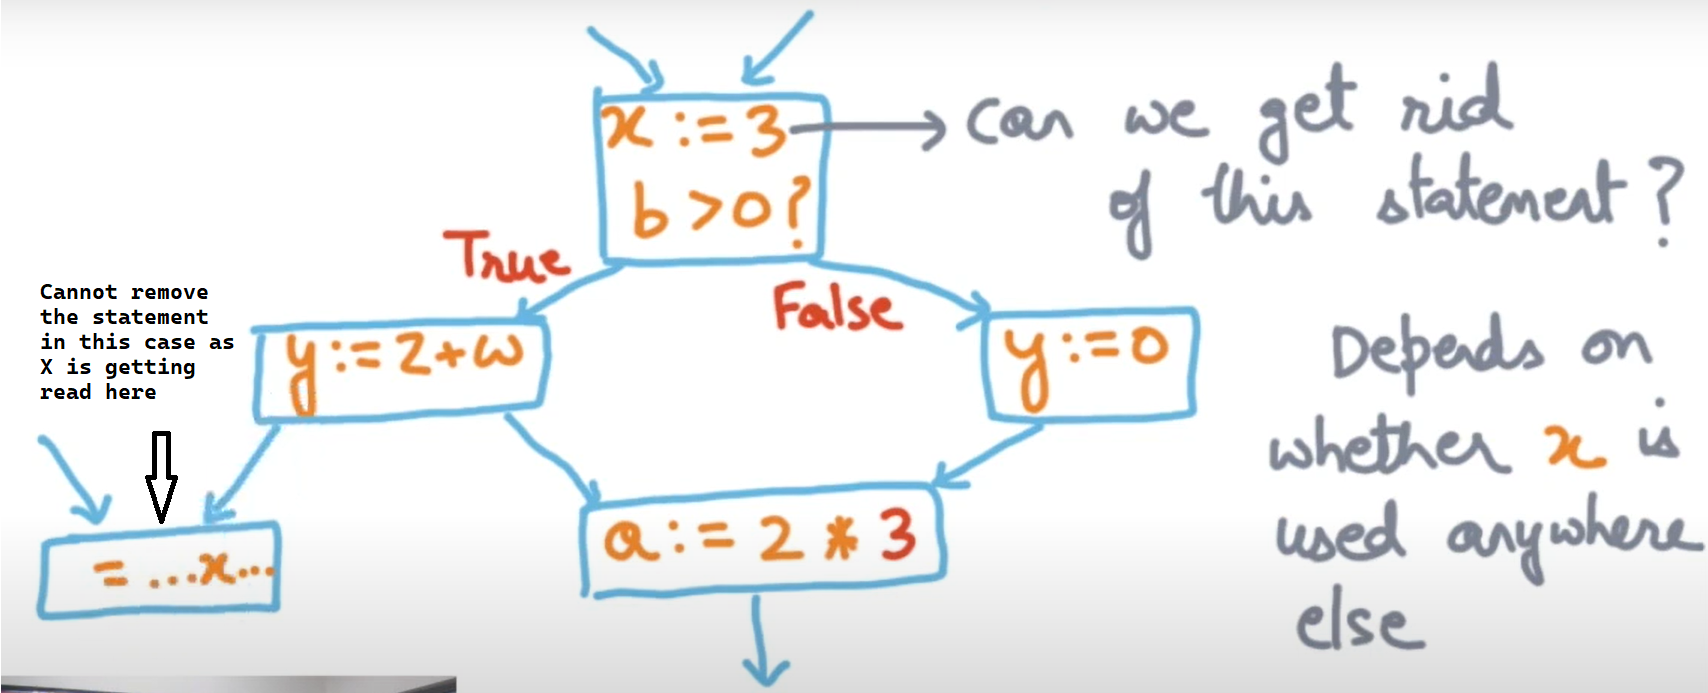
\includegraphics[height=6cm]{images/Module81_1.png}
    \caption{Motivation for Liveness Analysis}
\end{figure}

Consider a statement $x := ...$\\
Questions to ask: Is $x$ live or dead just after the statement? What does liveness mean?\\
Ans: A variable $x$ is live after a statement if it can be used in the downflow logic\\

Consider the following example:
\begin{figure}[H]
    \centering
    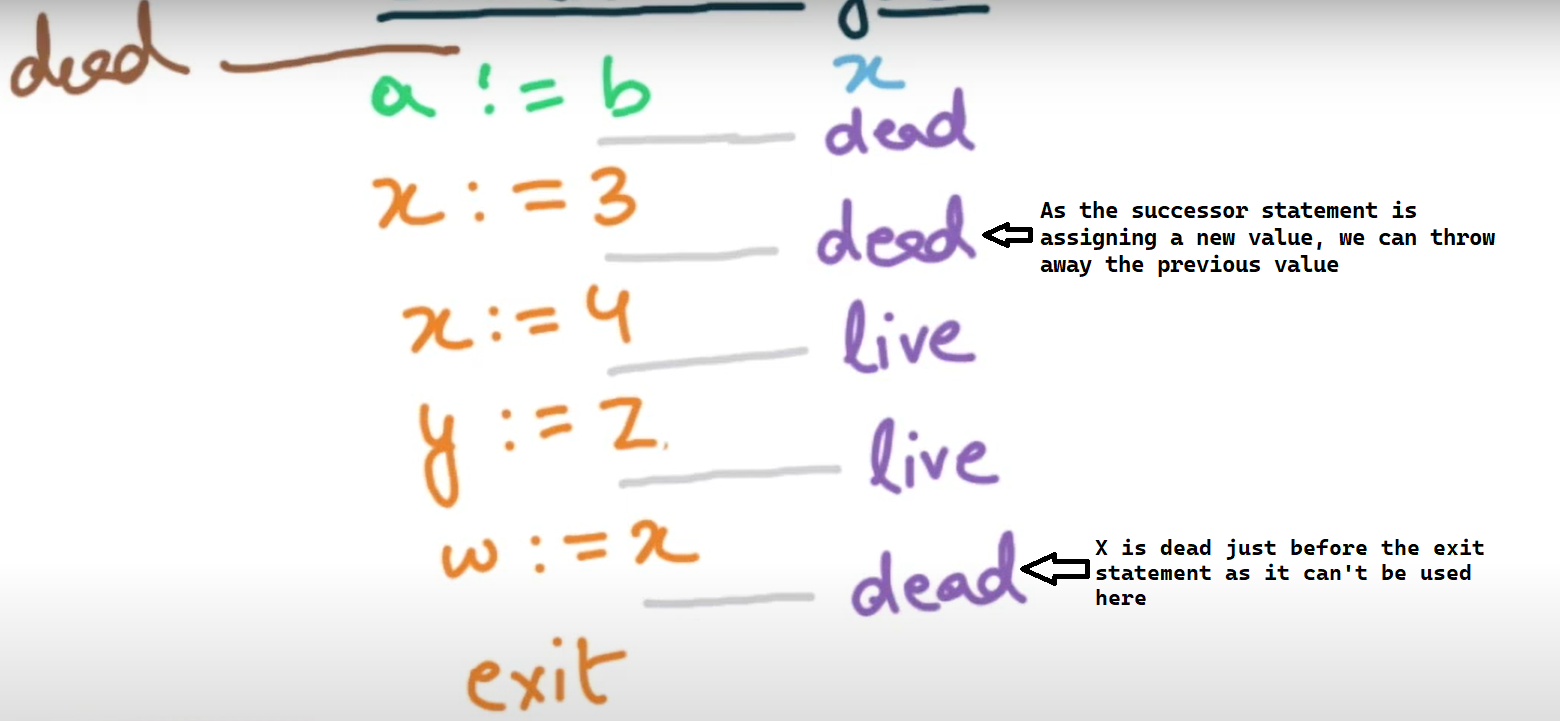
\includegraphics[height=6cm]{images/Module81_2.png}
    %\caption{Converting to SSA Example}
\end{figure}

\vspace{0.3cm}
The above intuition can be formalized as follows. A variable $x$ is live at a statement $s$ if:
\begin{itemize}
    \item There exists a statement $s'$ that uses $x$
    
    Eg:- $s':$ $y := f(...,x,...)$
    \item There is a path from $s'$ to $s$ (directed)
    \item The path has \underline{no intervening assignments} to $x$
\end{itemize}

Once we have figured if a variable $x$ live or dead at all statements, then we can easily identify dead code.\\
A statement $x := ...$ is dead code if $x$ is dead immediately after the assignment.
In this case, as the variable is not being used in the downflow logic, which means that we can simply remove the assignment.

\subsection{Liveness Analysis as a DFA}
In this analysis, the property that we want to know at a particular program point is the liveness of a particular variable. In the example above, we found the liveness value at one point using the other values.
This gives us an intuition for a $\textbf{Transfer Function}$, and hence we use a DFA for this problem as follows:
\begin{itemize}
    \item Express liveness at a program point based on the liveness of the successor program point (Backward Dataflow)
    \item The Liveness property for a variable $x$ would take a boolean value
    
    \hspace*{0.1 in}${\tt true} \rightarrow$ The variable may be live (This is a conservative value)\\ 
    \hspace*{0.1 in}${\tt false} \rightarrow$ The variable is definitely dead (not live)
\end{itemize}

\subsection{Ordering of Liveness Values}
As seen previously, it really helps to construct a partial ordering because it makes the rules concise. So we do would the same here. Define the ordering as:

\begin{center}
    ${\tt true} \leqslant {\tt false}$
\end{center}
\begin{figure}[H]
    \centering
    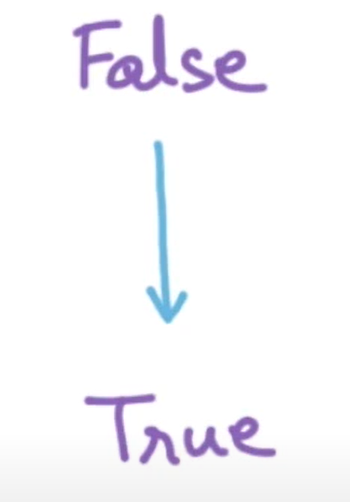
\includegraphics[height=2cm]{images/Module81_3.png}
    \caption{The Semilattice of Liveness Values}
\end{figure}

Once this ordering has been established, it can be easily seen that the greatest lower bound of any $2$ values $x, y$ would be the boolean OR of those values.
$$glb(x,y) = x \vee y$$
$$glb(x_1,x_2,...,x_n) = x_1 \vee x_2 \vee ... \vee x_n$$

 
%\setlength{\parindent}{0pt}

\clearpage
\section{Liveness DFA rules}
Now here we will define the transfer function for the Liveness Analysis. Define the function $L(s,x,in/out)$ as follows:

\begin{itemize}
    \item $x$ - the variable for which we want to compute the liveness values
    \item $s$ - a program statement $s$
    \item $in/out$ - whether it is input to the statement or output to the statement i.e just before the statement or just after the statement.
    \begin{itemize}
        \item $L(s, x, in)$ = The liveness value of x just before s
        \item $L(s, x, out)$ = The liveness value of x just after s i.e just after statement s is executed
    \end{itemize}
\end{itemize}

As discussed before, $L(s,x,in/out) \in \{{\tt true}, {\tt false}\}~\forall s,x$.\\

From now on, the discussion is for a particular variable $x$, but it can be generalized to more than one variables. We are going to define rules for the following 2 cases:

\begin{itemize}
    \item \textbf{Case 1:} A statement $p$ has one or more successor program points. So in this case, the $out$ value of the statement $p$ is expressed as a function of $in$ values of the successor program points.
    \item \textbf{Case 2:} For a given statement $s$, the $in$ value is a function of the $out$ value of that statement.
\end{itemize}
It can be obseved from here that unlike Global Constant Propagation, which is a Forward Dataflow Analysis, this is a Backward Dataflow Analysis (it starts from the exit point).

\subsection{Rules for the Transfer Function:}
%Insert Images
\begin{itemize}
    \item $L(p, x, out) = glb\{L(s_i, x, in)~|~s_i$ is a successor of $p\}$
    %Insert Image
    If $x$ is live before any of the successors, then $x$ is live after that statement as it may get used in the downflow logic.
    \item If $s$ is of the form $... = f(...,x,...)$, then $$L(s, x, in) = {\tt true}$$ as the variable $x$ is getting used in this statement.
    \item If $s$ is of the form $x := e$, where $e$ is an expression which does not refer to $x$, then $$L(s, x, in) = {\tt false}$$ as we don't need the values of $x$ just above this statement due to $x$ being rewritten
    
    Note: If $e$ referred to $x$, then Rule \#2 would apply
    \item If $s$ does not refer to $x$ at all (neither updating it, nor using it), then $$L(s, x, in) = L(s, x, out)$$
\end{itemize}

These rules are exhaustive. These can be thought of as a system of equations, and our solution should satisfy all these rules.

\subsection{Liveness DFA Algorithm}
\begin{itemize}
    \item Initialize $L(s, x, in/out) = {\tt false}$ for all statements $s$ and variables $x$ (We start from a more aggresive value)
    \item Repeat until all program points satisfy Rules 1-4
    \begin{itemize}
        \item Pick a statement $s$ not satisfying one or more rules in rules 1-4 and update the corresponding $L()$ function value using the appropriate rule
    \end{itemize}
\end{itemize}

There is a guarantee that this algorithm will converge.
%\setlength{\parindent}{0pt}

\section{Liveness DFA example}

Consider the following example:

\begin{framed}
    \hspace*{0.2 in} $x := 0$\\
    \hspace*{0.2 in} ${\tt while}(x~!=~0)\{$\\
    \hspace*{0.4 in} $x := x + 1$ \\
    \hspace*{0.2 in} $\}$ \\
    \hspace*{0.2 in} ${\tt return}$\\
    
\end{framed}
 
%Example CFG

\subsection{Liveness DFA Observations}
\begin{itemize}
    \item Every $L()$ in this analysis can change only once (${\tt false} \rightarrow {\tt true}$). Now this fact guarantees the convergence of the fixed point algorithm.
    \item Worst Case execution time: For a particular variable, all the $L()$ can change only once, and as the number of such values is $2 \times \#$statements, so the worst case execution time is $O(2 \times \#$statements).
    \item Once this analysis is finished, we can use it to identify dead code.
    \item Notice that information flowed in the forward direction (in the direction of the program execution) for constant propagation but flowed in the reverse direction (against the direction of the program execution) for liveness analysis.
    The former types of analyses are called forward dataflow analyses. The latter types of analyses are called backward dataflow analyses
\end{itemize} 
%\setlength{\parindent}{0pt}
\clearpage

\section{More DFA Examples}

\subsection{Common Subexpression Elimination}


In this analysis, the property that we want to know at a program point is all the expressions available at that point.
\begin{itemize}
    \item The idea is to maintain a set of available expressions and the temporary in which they are stored, for every program point
    \item If a subexpression is available in the set of available expressions just before the statement that computes that subexpression, then replace it by the corresponding temporary (the precomputed value)
\end{itemize}

%Insert Examples

\subsection{Available expressions DFA}
In this analysis, the DFA value that we will deal with is a \underline{set of available expressions}, where each element in this set is a tuple of the register and the expression stored in that register.

So $(x, y+z)$ denotes that the value of the subexpression $y+z$ is stored in the temporary $x$.

\vspace{0.5cm}
Here also we will set a partial ordering in the values as follows:\\
$$s_2 \leqslant s_1 \textbf{ iff } s_2 \subseteq s_1$$

The lowest value in this ordering is $\{\}$, the empty set. This is a conservative value as it denotes that there is no Subexpression available, hence no subexpression available.

Once this ordering has been established, we can easily see that $glb(s_1,s_2) = s_1 \cap s_2$.

\subsection{Transfer Function for Available Expressions}
This happens to be a forward dataflow analysis, so we will have 2 types of rules:

\begin{itemize}
    \item \textbf{Case 1:} A statement $s$ has one or more predecessor program points. So in this case, the $in$ value of the statement $s$ is expressed as a function of $out$ values of the predecessor program points.
    \item \textbf{Case 2:} For a given statement $s$, the $out$ value is a function of the $in$ value of that statement.
\end{itemize}

Define $set_{in}(s)$ be the set of available expressions before the statement $s$, and $set_{out}$ be the set of available expressions after the statement $s$. The transfer function has the following rules:

\begin{itemize}
    %insert images
    \item If $s$ is $x := y + z$, then remove all the set elements that refer to $x$ (all the expressions stored in $x$ and using $x$) from $set_{in}(s)$. Then add $(x,y+z)$ to $set_{out}(s)$.
    \item For a statement $s$ and it's predecessors, $set_{in}(s) = glb\{set_{out}(p_i)~|~p_i~\in~{\tt predecessor}(s)\}$
\end{itemize}

Also if $s$ is the starting statement, then the boundary condition for this algorithm would be $set_{in}(s) = \{\}$.

\subsection{Copy Propagation}
Copy Propagation can be easily modelled as a DFA analysis very similar to Available Expressions DFA, except that we will be limiting ourselves to statements of the form $x := y$. The transformation logic will also be similar.\\

This optimisation creates oppurtunities for other global optimizations such that Global Constant Propagation and Liveness Analysis, so it works well in tandem with them.


%\section{Module 85: Register Allocation}
\begin{flushright}
\textit{(scribed by Jai Javeria)}
\end{flushright}
The Intermediate Representation uses an unlimited number of temporaries. While this simplified code generation and optimization, a machine only has  finite resources and thus we need to map potentially large number of temporaries with the machine registers.

\subsection{Many to One Mapping}
\begin{itemize}
    \item Since there are more temporaries than registers, we would have to assign multiple temporaries to a single register without changing program behavior. 
    \item If this is not possible then we have to store('spill') some of the temporaries in the memory.
    \item We can have a static mapping, where a temporary is mapped to the same register for the entire duration of the execution of code. We can also dynamically allocate registers, assigning a temporary to a register at one program point, "spilling" it to memory at another program point and assigning it back to a different registers at a different program point.
    \item A static mapping is simpler to implement that a dynamic one. For now we would focus on it and later think about relaxing this assumption (that one temporary is assigned to only 1 register).
\end{itemize}
\subsection{Register Allocation Example}
Lets take the following code:\\
% \begin{algorithm}[H]
% \SetAlgoLined
\begin{center}
    // Some code\\
    a:=c+d\\
    e:=a+b\\
    f:=e-1\\
    // Some more code\\
\end{center}
The only temporaries are a-f.
Also assume a,e are dead after the  last line and we have 4 registers available for allocation.\\
A possible allocation can be.
\begin{center}
    a, e, f $\rightarrow$ r1\\
    c $\rightarrow$ r2\\
    d $\rightarrow$ r3\\
    b $\rightarrow$ r4\\
\end{center}
The new transformed code would be
\begin{center}
    r1:=r2+r3\\
    r1:=r1+r4\\
    r1:=r1-1\\
\end{center}
How do we know that this is correct?
\begin{itemize}
    \item In the first line a is computed correctly in r1. In the second line e is computed correctly and stored in r1.
    \item But since r1 is overwritten, value of a is no longer available, which is ok since a was dead after the second line in the original code as well.
    \item In the third line, value of f is correctly computed and stored in r1. Value of e is no longer available which is not wrong since it is given e is dead after this line.
\end{itemize}
\textbf{Insight}: We could map a,e,f to the same register r1 because at no program point they are live simultaneously.\\
\textbf{Idea}: Temporaries t1 and t2 can share the same register \textbf{iff} at all program points, atmost one of t1 and t2 is live.
\subsection{Another Example}
Consider the following example:\\
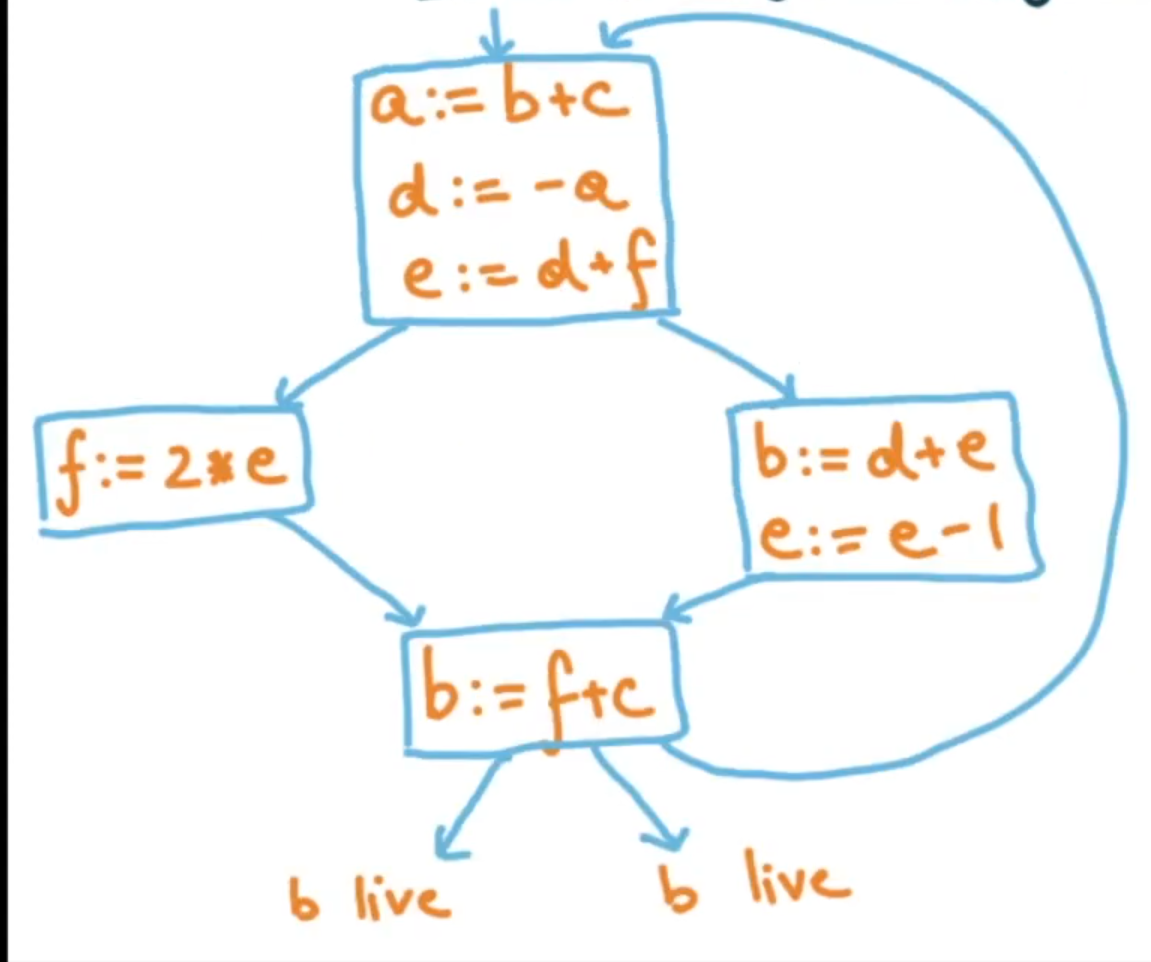
\includegraphics[scale=0.2]{images/85_eg.png}\\
The above image represents the control flow graph of the program under consideration.\\
Executing a liveness analysis on the program we get:\\
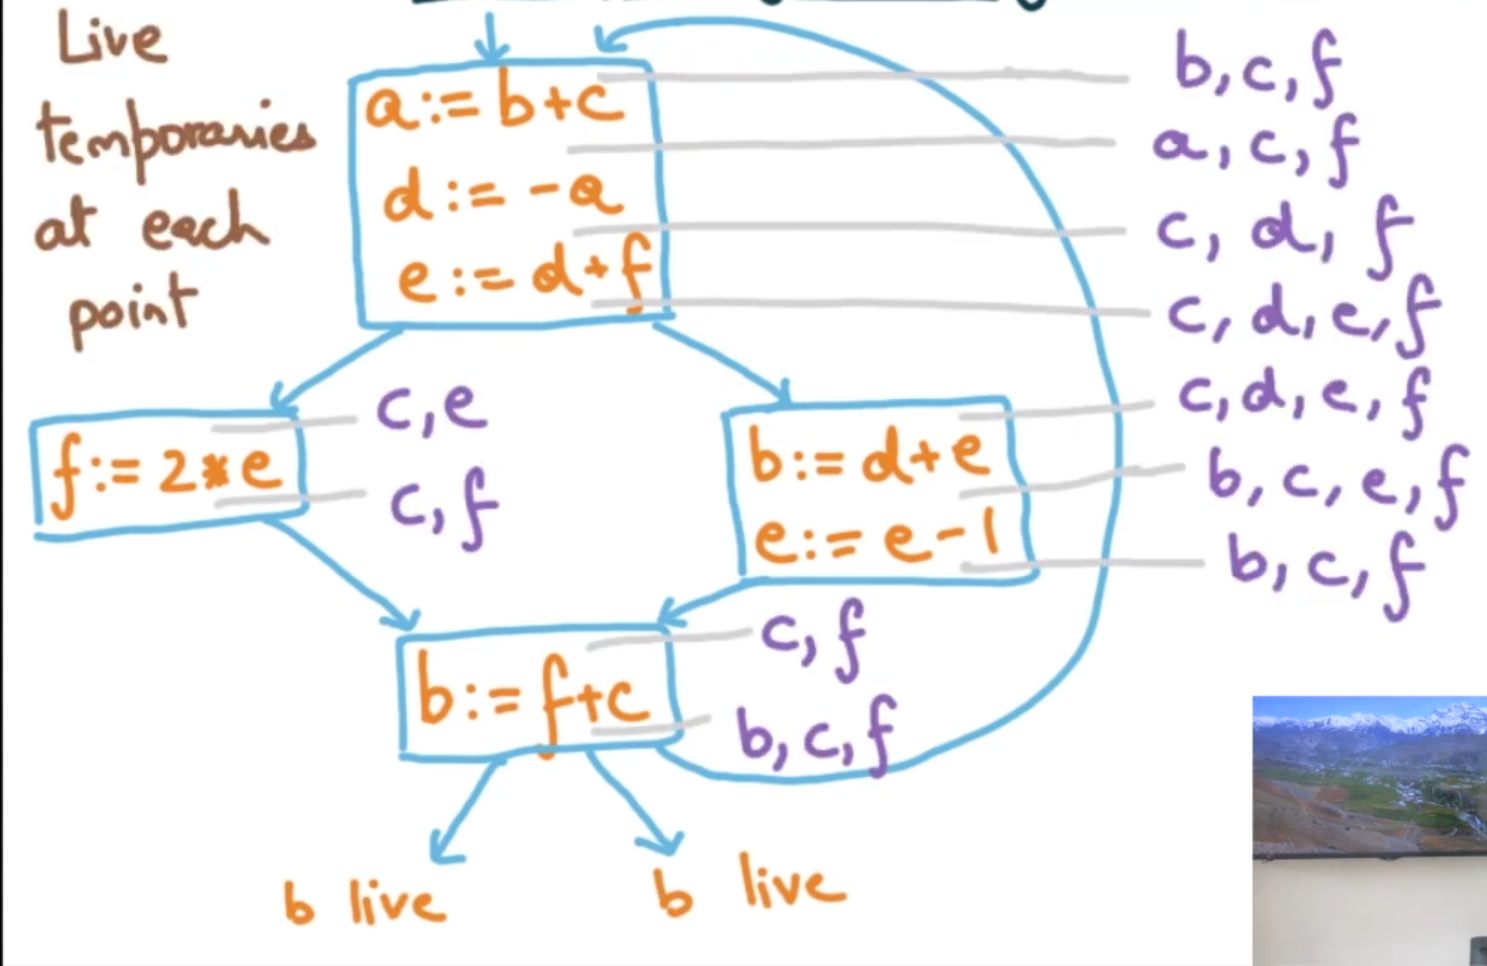
\includegraphics[scale=0.2]{images/85_eg2.png}\\
Everything in the purple pen represent the variables that are live at that particular program point.\\
Now we need to find the pairs of variables that are not live simultaneously at any program point. After going through the program points above, we see that the following pairs of variables are not live simultaneously.
\begin{itemize}
    \item (a,b)
    \item (b,d)
    \item (a,d)
    \item (a,e)
\end{itemize}
These pairs of variables can share a register. Moreover, from the pairs (a,b), (b,d), (a,d) we can infer that a,b,d can be allocated to the same register. \\
Next, we discuss an algorithm for register allocation from the ideas that we got from the two examples.
\subsection{Towards a Register Allocation Algorithm}
\begin{itemize}
    \item Construct an undirected graph.
    \item Node for every temporary
    \item There is an edge between t1 and t2 if they are simultaneously live at some program point.
    % \item Color the graph with k colors, where k is the number of registers. If this is possible we 
\end{itemize}


The undirected graph made is called as Register Interference Graph (RIG). If 2 temporaries do not have an edge between them then we can allocated them to the same register.\\
The RIG for the second example discussed above is\\
\begin{center}
    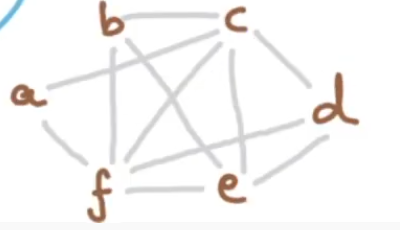
\includegraphics[scale=0.2]{images/85_RIGeg2.png}\\
\end{center}
As we can see that the RIG extracts a global picture from the program. Now we do not need to be concerned about any program point.\\
For any register allocation to be valid, any 2 temporaries mapped to the same register by the allocation must not have an edge between them.\\
% Motivated from this we can see Graph Coloring can help us in getting an allocation.\\
Lets just deviate and discuss a theoretical computer science problem.\\
\textbf{Graph Coloring:} An assignment of colours to each node of the graph so that nodes connected by an edge do not have the same color.\\
\textbf{k-colourable Graph:} A graph is k-colourable if it can be coloured with k colours.\\
On giving it a thought, we can see that the problem of graph colouring can help in validating if a register allocation is possible. Denote every register with a unique colour and try to colour the RIG with k colours, where k is the number of registers. If it is possible we get a valid register allocation for each temporary, else we need to spill some temporaries to memory.\\
% Unfortunately graph colouring is a NP hard problem. In the next module we discuss a heuristic based   
%\section{Module 86: Register Spilling}
\begin{flushright}
\textit{(scribed by Jai Javeria)}
\end{flushright}
What do we do when we do not get a valid k colouring for a graph. In such a case we need to save some registers in the memory and update our code accordingly.\\
\textbf{Note:} Graph colouring is a NP hard problem and we would generally use some heuristic to find a colouring.  It might be the case that there exist a k colouring for the graph but our heuristic is not able to find it. In this case also we would spill registers to the memory.\\
\subsection{Register Allocation with Spilling}
\begin{itemize}
    \item Try to colour the RIG with k colours (k=number of machine registers).
    \item If this is not possible, pick up a node as a candidate for spilling.
    \item This register will now live in memory. Remove the picked node and all of its incident edges from the RIG.
    \item Repeat until the graph becomes k colourable.
\end{itemize}
The idea behind this algorithm is that when we remove one node from the RIG, it becomes sparser and hopefully it would become k colourable now. The algorithm is guaranteed to work because in the worst case the RIG would become k colurable when it has only k nodes left.
\subsection{Which node to pick}
\begin{itemize}
    \item The main idea to pick the node is to make the graph sparser and thus k-colourable. So one could pick the node with the maximum edges. This would make the RIG most sparser one at a time and we can get our solution faster.
    \item But it could happen that the node we picked up represents a register value that is used extensively in the code. This variable should not be sent to live in the memory, otherwise the runtime memory accesses would increase. Thus a better alternative is to select a register which has the minimum static live range i.e. all the program points where it it live.
    \item But a variable used just in a loop would have a less static live range but if the loop runs a million times during runtime, it would be not good to store it in memory. Thus we could select registers to spill based on 'cold' regions, the regions which are not going to be executed many time during runtime, e.g. the initialization part of the code.
    \item But just looking at the code statically may not give an accurate picture of which regions are cold and hot. Thus often a combination of 2nd and the 3rd strategy is used for selecting nodes. A JIT (Just In Time) compiler has an advantage of determining cold and hot regions more accurately.
\end{itemize}
\subsection{Optimistic Colouring}
\begin{itemize}
    \item Pick a node to spill, say n, and remove it and its edges from the RIG.
    \item Colour the remaining graph with k colours ( by potentially spilling more nodes).
    \item After we have got a colouring, try to put n back into the graph such that we can find a colour for n too.
\end{itemize}
\subsection{Optimistic Colouring Example}
Lets take the RIG example from the previous module
\begin{center}
    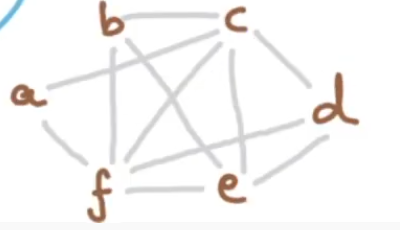
\includegraphics[scale=0.30]{images/85_RIGeg2.png}
\end{center}
And lets say we only have 3 registers for allocation and thus we need to find a 3 colouring. The current graph is not 3 colourable and thus we pick a node for spilling, say a.
\begin{center}
    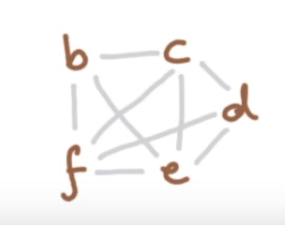
\includegraphics[scale=0.30]{images/86_remove_a.png}
\end{center}
We see that again the graph cannot be coloured in 3 colours and thus we select another node for spilling, say f. Now we can colour the graph with 3 colours.
\begin{center}
    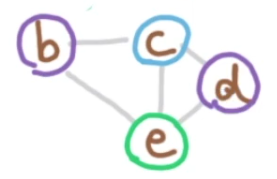
\includegraphics[scale=0.30]{images/86_color_RIG.png}
\end{center}
Now we try to add f back to the graph, but we cannot find a colour for f.
\begin{center}
    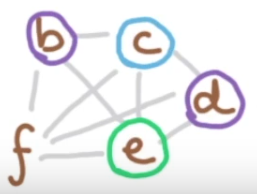
\includegraphics[scale=0.30]{images/86_add_f.png}
\end{center}
We move to adding a to the RIG and we are successful in colouring it.
\begin{center}
    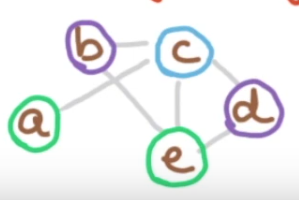
\includegraphics[scale=0.30]{images/86_add_a.png}
\end{center}
Thus finally we need to spill f to the memory.
\subsection{How to Spill}
\begin{itemize}
    \item Allocate a memory location for f on the stack frame. Let its address be $f_a$
    \item Before each operation that reads f, insert
        \begin{center}
            f = load $f_a$
        \end{center}
    \item After each write operation on f, insert
        \begin{center}
            store f, $f_a$
        \end{center}
    \item Also rename every use of f to f1,f2... . This would be beneficial for some further analysis that needs to be done. Since each different instance of f would be getting different values, it is possible to rename them to different variables.
\end{itemize}
\subsection{Effect of Spilling on RIG}
Since we have broken down f into different variables with short live ranges, the graph becomes sparser and easier to colour.

%\section{Module 87: Limitations of Graph Colouring}
\begin{flushright}
\textit{(scribed by Jai Javeria)}
\end{flushright}
\begin{itemize}
    \item Register Allocation is done statically. 
    \item Our allocation suffers from the all-or-nothing problem i.e. a temporary is allocated to a register at all program points or none at all.
    \item Suppose a temporary t1 is used twice in the program. Once inside a loop and the other in a non loop branch. The loop might execute a million number of times and it is essential for t1 to be in a register for performance whereas the second occurrence of t1 in a non loop statement, which might be taken only a few number of times, can have it stored in the memory without much loss of performance.
\end{itemize}
\subsection{Region Based Register Allocator}
Partition the program into regions; solve for each region seprately and reconcile at region boundaries.
\subsubsection{How to partition into Regions}
\begin{itemize}
    \item One region for each loop body.
    \item Regions based on register pressure. Divide the code into regions based on how many number of registers are being used. In one region the register pressure is high and thus we need to spill some temporaries into the memory whereas in some other region, the register pressure is low and thus we can bring everything back to the register file.
\end{itemize}
\subsubsection{Limitations}
\begin{itemize}
    \item There is an overhead of reconciliation at a region boundary. For correctness we need to do a translation from one mapping to the other at a region boundary and thus the regions selected should not be too small.
    \item We also need to do instruction selection later. But some instructions only operate on specific registers and if the operands are not in the required registers, then we somehow need to go back to register allocation again to fix this.
    \item Some fixes are there for example the reloading pass in the GCC compiler. If there is some problem with the register allocation during the instruction selection then GCC has some architecture specifc rules on how to transform the code to something that would work.
    \item \textbf{Alternative Approach} Do register allocation and instruction selection simultaneously. We can use dynamic programming approaches that looks at what instructions can be used to implement the given functionality of a subset of IR code and at the same time would look into how can register allocation be done and then somehow combines both to get a solution.
    \item This involves some more complexity and adds compilation time but can also generate significantly better results.
\end{itemize}
 
%\section {Alternate DFA Representation}
\setlength{\parindent}{0pt}

(Prepared by Sameer V. Pande)

\vspace{0.3cm}


In all the modules till now, we've focussed on DFA algorithms which focus on just one variable at a time. 
For example, in constant propagation we try to propagate information about value of a variable ( $\top$/ $\bot$/ constant) throughout our CFG. 
\newline\newline
We need alternate representations of DFA because of the following reasons :
\begin{itemize}
    \item Increase the efficieny by analysing multiple variables at once.
    \item Develop a common framework/structures, with the help of which we can built a lot of DFA algorithms and reason about their properties (like optimality, precision).
\end{itemize}

Representing constant information using sets to keep track of multiple variables simultaneously is one example of alternate representation of DFA.
We store a set of tuples, where first value of tuple is the variable and the second variable is the value of the variable.
One of the optimizations of this representation is that absence of a variable from a set indicates that its value is $\bot$/. Let's see an example program to understand this alternate DFA representation.

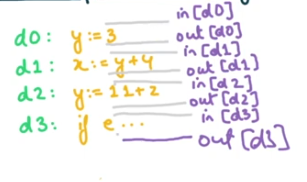
\includegraphics[scale=0.50]{88_1.png}

For each program statement, we define two program points : in and out. The information sets propagated to the program points are as follows :
\begin{itemize}
    \item \textbf{in[d0]: \{\}}
    \item \textbf{out[d0]: (in[d0] - \{(y,*)\}) $\bigcup$ \{(y,3)\}}
    \item \textbf{in[d1]: out[d0]} 
    \item \textbf{out[d1]: f(in[d1])}
    \newline where f represents the tranfer function. If f is "intelligent" then it can deduce that \textbf{x} should have value \textbf{7}. Whereas a less sophisticated would remove all tuples corresponding to variable x, since x has been overwritten
    \item \textbf{in[d2]}: out[d1]
    \item \textbf{out[d2]}: in[d2] - \{(y,*)\}
    \item and so on ...
\end{itemize}

\textbf{Meet Operator}: Meet operator is used in data-flow analysis to compute \textbf{in[node]} (\textbf{out[node]}) when there are multiple incoming (outgoing edges), with help of outsets (insets) of incoming (outgoing) edges in forward (backward) dataflow analysis.
Meet function is same as greatest-lower-bound (glb) function over the inputs. For constant-propagation the glb has to be set-intersection operator.
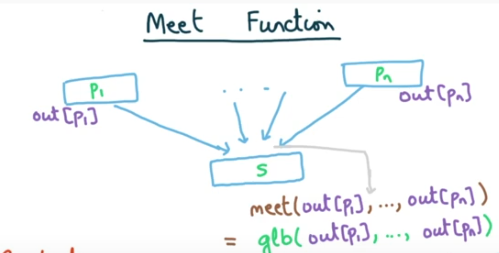
\includegraphics[scale=0.5]{88_3.png}

Summarizing the lecture, out[s] = f(in[s]), where f is the transfer-function. And very often \textbf{out[s] = (in[s] - kill[s]) $\bigcup$ gen[s]}. Note that kill and gen sets depend only on statement s. Killing before generation is also important for correctness of the analysis.
%\section {Gen and Kill Sets}
\setlength{\parindent}{0pt}
(Prepared by Sameer V. Pande)

\subsection{Transfer and Meet Functions}
In previous module we discussed about how a DFA can be expressed with help of transfer and meet functions.
Transfer function computes the value of out[s] as a function f(in[s]). And for forward dfa, when there are multiple incoming edges at a node,
the meet operator computes the in[s] as a function of outsets of the predecessors.

\subsection{Using GEN and KILL sets to represent transfer functions}
In most cases, it is possible to represent transfer function with help of gen-sets and kill-sets which depend only on the statement (hence, can be computed statically).
Transfer function 'f' can be written as: \textbf{f(V) = (V - Kill(s)) $\bigcup$ Gen(s)}. The first part of expression
\textbf{ V - Kill(S)} is called "propagate" part and \textbf{Gen(S)} is called 'generate' part.

\subsection{Examples of Gen and Kill Sets}
We'll see two examples of gen/kill sets 
\subsubsection{Constant Propataion}
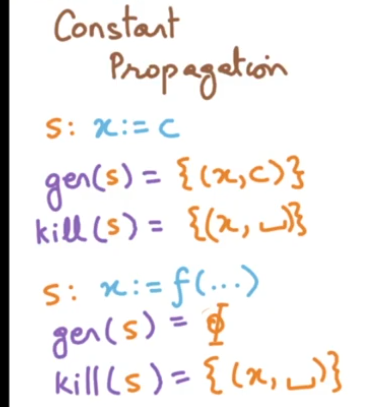
\includegraphics[scale=0.5]{images/89_1.png}
\newline 
The gen-set for constant-assignment is just \{(x,c)\}. The kill-set ensures that any previous value of the variable x is removed from the set, before new value is added via gen.
When x is assigned a value via a complex function/expression, then gen-set is empty-set but kill-set removes the old value of x, if any.
\subsubsection{Available Expressions Analysis}
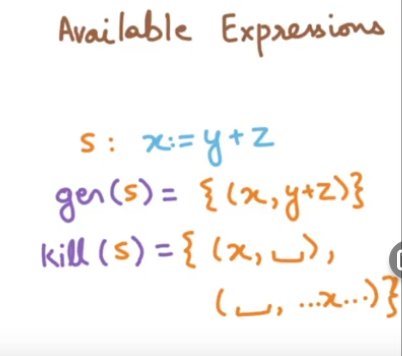
\includegraphics[scale=0.5]{images/89_2.png}
\newline 
Consider case when variable x is assigned an expression. The gen-set is similar to that of constant propgation (but now it has expressions as well, instead of just constants). The kill-set takes care of two things 
\begin{enumerate}
    \item Remove the expressions corresponding to variable x 
    \item Remove the variables which have expressions corresponding to older-value of x.
\end{enumerate}

\subsection{Gen/Kill Summaries for Basic Blocks}
One of the advantages of using basic-blocks is that it generates summaries over the entire block. We can take a sequential composition of transfer function of all statements in the basic-block to give us a block-level transfer function.
A block level transfer function can be represented using block level genset and killset.
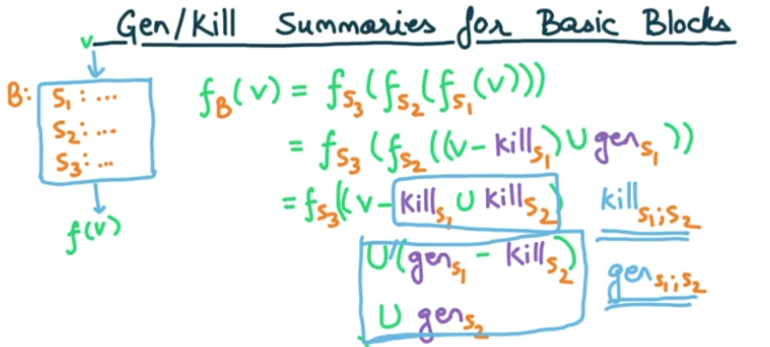
\includegraphics[scale=0.5]{images/89_3.png}

For a basic block B, Gen$_B$ and Kill$_B$ can be interpreted as follows:
\begin{itemize}
    \item Gen$_B$: Locally exposed constant definitions,i.e., the definitions available at the end of basic-block B.
    \item Kill$_B$: Set of constant definitions killed by B.
\end{itemize} 
%\section {Reaching Definitions}
\setlength{\parindent}{0pt}
(Prepared by Sameer V. Pande)

Reaching definitions is a more-detailed dataflow analysis, which contains the "possible" definitions a variable can take at a program point, unlike available-expression analysis, which indicates the value that a variable definitely takes.
This is more fine-grained because it doesn't declare variable values as $\bot$ when a variable can potentially have more than one value (depending on the path taken to reach the point), unlike available-expression analysis.
\newline 
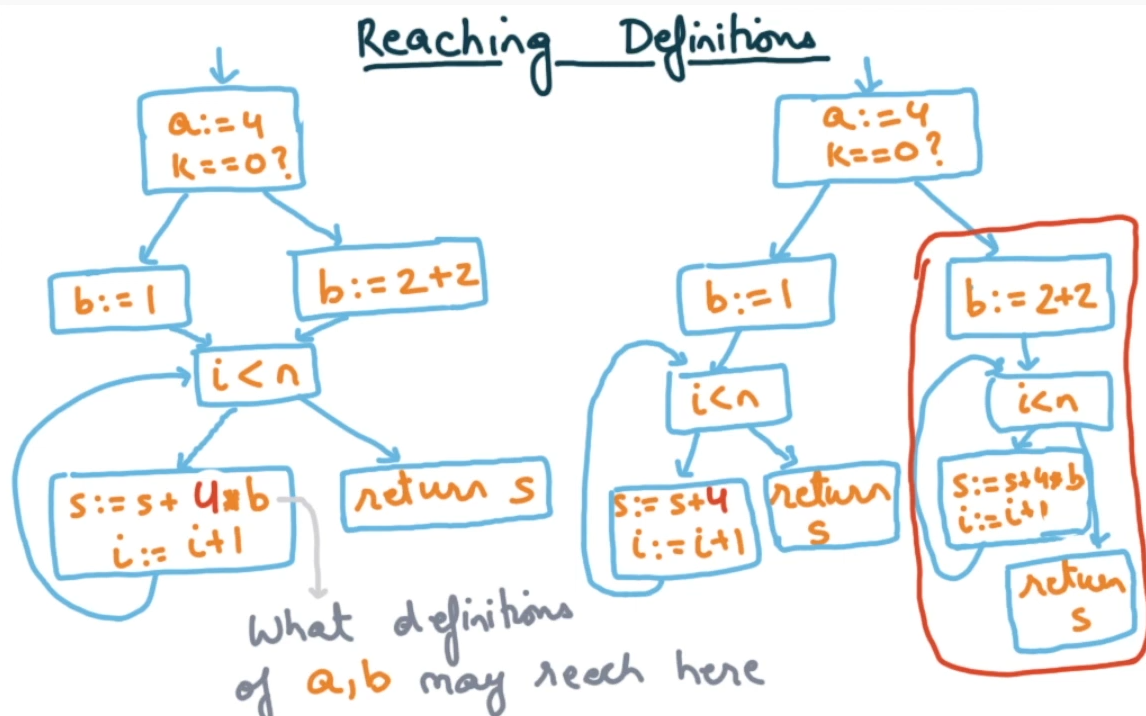
\includegraphics[scale=0.3]{images/90_1.png}

Consider the example above, and assume that program usually spends most of its execution time in the loop. In the loop, the variable "b" can have two values "1"/"y+z". If we use reaching-definitions analysis we can know that only two values of "b" are possible (one of which is a constant) and we can \textbf{specialize} the code (as seen in right-figure), by replicating the branch and specializing one of the branch on a constant value of b.

\subsection{Gen/Kill Sets and Meet for Reaching Definitions}
It is a forward dataflow analysis. Gen(S) of a statment S, contains all the new definitions generated by the S. And kill contains all definitions killed.
Hence for the example "S:x=y+z", Gen(S) = \{(x,y+z)\} and Kill(S) = \{(x,*)\}.
\newline
In reaching definitions the \textbf{meet operator is union}. Meet is union operator because we want the definitions which can reach the program point via \textbf{any} path. 

\subsection{Reaching Definitions vs Available Expressions}
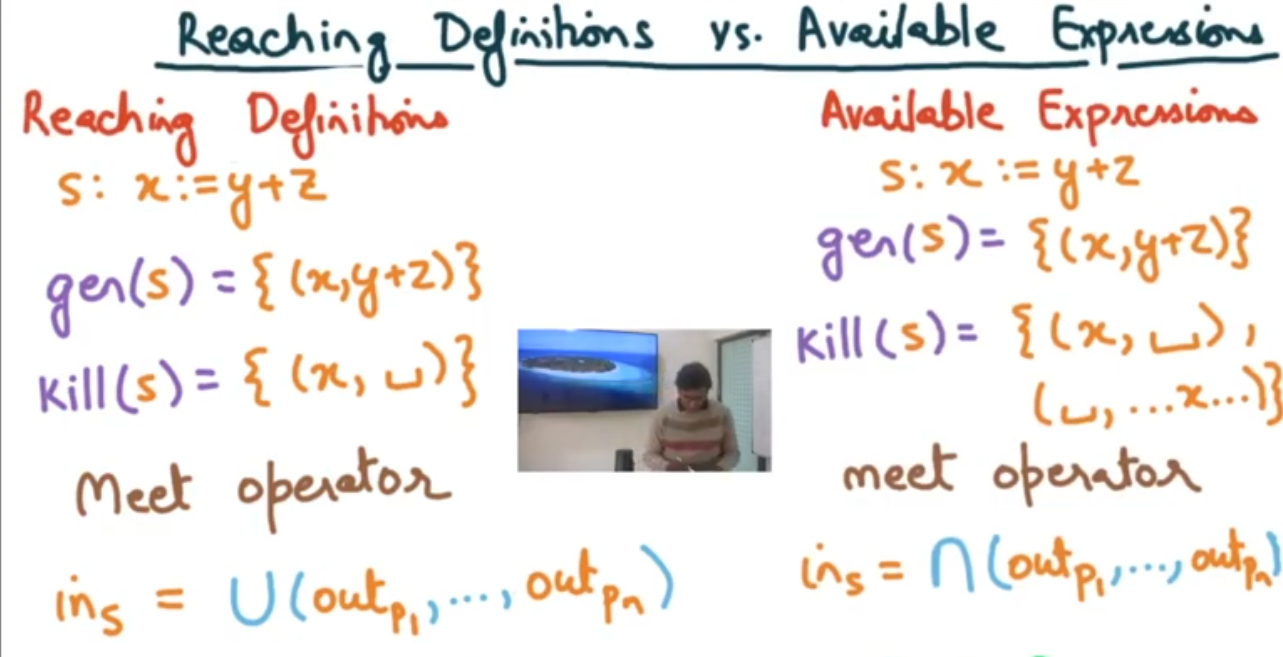
\includegraphics[scale=0.3]{images/90_2.png}
It is important to note that "Reaching-Defintions" is analysis involving definitions and "Available-Expressions" involves expressions.
From above figure, we can see that Gen() is very similar for both. But there are important differences in the following 
\begin{itemize}
    \item Kill Set: In addition to (x,*), available-expressions also kills (*, ...x...) i.e. all variables with values dependent on previous value of x. This is not present in reaching-defintions since we are only worried about "definitions", we don't have to deal with this case (where x also appears in rhs). 
    \item Meet Operator: The meet operator of reaching definitions is \textbf{union} because we want to consider \textbf{any} defintion of a varialbe that can reach at current program point \textbf{through any path}. 
    Whereas available-expressions requires the same expression to reach the current program point through \textbf{all possible paths}. Hence \textbf{intersection} is suitable for available expressions. 
\end{itemize}
%\section {Introduction to DFA Framework}
\setlength{\parindent}{0pt}
(Prepared by Namrata Priyadarshani and Shivam Bansal)

\vspace{0.3cm}

In this module, we build up common framework to express DFA. Some common characteristics of DFA are described below: 

\subsection{Transfer Functions and Meet operator}

Let s be a statement and the value before statement is in[s] and after statement is out[s]. Then, for a forward DFA, \textbf{Transfer function} is defined as the function that takes in[s] as argument and converts it into out[s]. \textbf{Meet operator} expresses in[s] as the function of out[p] for all predecessor p of s. These functions operates in reverse direction in the case of Backward DFA.
\newline
Most of the time, we consider running the algorithm at the Basic Block level granularity and define Transfer function and meet operator for the values in[B] and out[B] i.e. the input and output values of the basic block B. 

\subsection{Partial ordered values}

There is a partial order within the elements of Domain represented by $\geq$ operator.
Directed Acyclic Graph is one way to represent the ordering. The graph contains an edge from $a \rightarrow b$ iff $a \geq b$.
%insert image
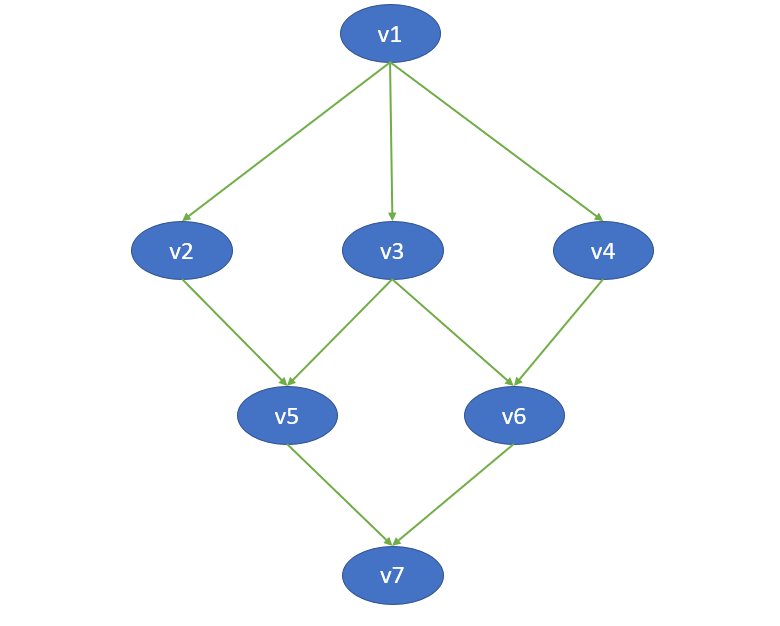
\includegraphics[scale=0.3]{images/91_1.png}
There is one value greater than all values in Domain known as Top value (T) and one value less than all values in Domain known as Bottom value ($ \bot $).

\subsection{Constant Propagation DFA}
Different DFA has different direction, boundary condition, meet operator and transfer function. The structure and flow of algorithm remains same for all DFA. In fixed-point-algorithm first the boundary condition is specified, all other values are set to top value and then iterate until no change occur in any value.

For constant propagation the DFA is specified by:
\begin{itemize}
    \item \textbf{Domain}: set of constant definitions
    \item \textbf{Direction}: Forward
    \item \textbf{Transfer function}: $f_{B} = \lambda x. GEN[B] \cup (x-KILL[B]) $
    \item \textbf{Meet operator}: $\cap$ (set intersection)
    \item \textbf{Boundary condition}: $out[entry] = \phi$
\end{itemize}
 
%\section {Live Variable Analysis}
\setlength{\parindent}{0pt}
(Prepared by Namrata Priyadarshani and Shivam Bansal)

\vspace{0.3cm}

In this module, we try to fit Live Variable Analysis, a backward DFA in the framework developed in previous lecture.

\begin{itemize}
    \item \textbf{Values}: set of variables that are live at a program point.
    \item \textbf{Transfer function}: It is defined in terms of Use and Def, where $Use[s]$ denotes the variable used in the statement s and $Def[s]$ denotes the variable defined.
    \newline
    For example: In statement $S: x=y+z$, $Use[S] = \{y,z\}$ and $Def[S] = \{x \}$.
    Let the value just above S be in[S] and just below S be out[S] and f be the transfer function, then $in[S] = f(out[S]) = Use[S] \cup (out[S] - Def[S])$. The generation here is $Use[S]$ and the propagation is $out[S] - Def[S]$.
    \newline
    \newline
    At Basic block granularity, $in[B] = Use[B] \cup (out[B] - Def[B])$, where $Use[B]$ is set of locally exposed uses in B and $Def[B]$ is set of variables defined in B.
    
    \item \textbf{Meet operator}: Meet operator is Set Union ($\cup$) as a variable is live if it is live on any of the outgoing paths. So, $out[B] = \cup in[s_{i}]$ $\forall i$ such that $s_{i}$ is the successor of B. 
    \newline
    The ordering is such that the less than equal to operator indicates the superset. The top value will be $\phi$ or empty set. The bottom value will be set of all variables.
    \item \textbf{Boundary Condition}: in[Exit] = $\phi$.
\end{itemize}

%\definecolor {processblue}{cmyk}{0.96,0,0,0}
\clearpage
\section{Reaching Definitions Example}
(Prepared by Namrata Priyadarshini, Shivam Bansal)

We've been looking at different types of data flow analyses and trying to tie them into a single framework. One of the data flow analysis that we looked at was reaching definitions and recall that a reaching definition basically is defined as follows:
A definition D of the form x = y + z reaches a point P in the program if there exists a path from the point immediately following D to P such that D is not killed, in other words x is not overwritten along that path. 
So even if there exists one such path where from the end of D to the beginning of P such that x has not been overwritten on that path then D would be considered to be to reach P. So let's look at this example:

\begin{figure}[h!]
\begin {center}

\begin{minipage}{.5\textwidth}
\centering
\caption{Control Flow Graph}
\begin {tikzpicture}[-latex ,auto ,node distance =3.5cm and 5cm ,on grid ,
semithick ,
state/.style ={ rectangle ,top color =white , bottom color = processblue!20 ,
draw,processblue , text=blue , scale = 0.7 ,minimum width =4 cm, minimum height = 4 cm}]
\node[state] (A){} node [label = {[label distance = 0.3cm]90:},rectangle split,rectangle split parts=1]{%
  d1 : b=3
  };
\node[state] (B) [below = of A]{} node [label = {[label distance = 0.3cm]90:}, rectangle split,rectangle split parts=1] [below = of A] {%
  d2 : c = 3
  };
\node[state] (D) [below =of B]{} node [label = {[label distance = 0.65cm]90:}, rectangle split,rectangle split parts=1] [below = of B] {%
  d3 : c = 4
  %
  };
\path[->] (A) edge node [below=0.3cm] {} (B);
\path[->] (B) edge node [above=0.3cm] {}  (D); 
\path[->] (B) edge [out=300,in=72,looseness=3] node[align = right][right] {} (B);
% \path[->] (B) edge [loop right] node {} (B) ;
\draw[->] (D) --++(0,-2.5cm) node [above left = 0.05cm] {} ;
\draw[<-] (A) --++(0,2.5cm) node [above left = 0.05cm] {} ;
\end{tikzpicture}
\end{minipage}%
\begin{minipage}{.5\textwidth}
\centering
\caption{Reaching definitions}
\begin {tikzpicture}[-latex ,auto ,node distance =3.5cm and 5cm ,on grid ,
semithick ,
state/.style ={ rectangle ,top color =white , bottom color = processblue!20 ,
draw,processblue , text=blue , scale = 0.7 ,minimum width =4 cm, minimum height = 4 cm}]
\node[state] (A){} node [label = {[label distance = 0.3cm]90:},rectangle split,rectangle split parts=3]{%
  $\Phi$
  \nodepart{second}
  d1 : b=3
  \nodepart{third}
  $\{d1\}$
  };
\node[state] (B) [below = of A]{} node [label = {[label distance = 0.3cm]90:}, rectangle split,rectangle split parts=3] [below = of A] {%
  $\{d1,d2\}$
  \nodepart{two}
  d2 : c = 3
  \nodepart{three}
  $\{d1,d2\}$
  };
\node[state] (D) [below =of B]{} node [label = {[label distance = 0.65cm]90:}, rectangle split,rectangle split parts=3] [below = of B] {%
  $\{d1,d2\}$
  \nodepart{two}
  d3 : c = 4
  \nodepart{three}
  $\{d1,d3\}$
  %
  };
\path[->] (A) edge node [below=0.3cm] {} (B);
\path[->] (B) edge node [above=0.3cm] {}  (D); 
\path[->] (B) edge [out=300,in=72,looseness=3] node[align = right][right] {} (B);
% \path[->] (B) edge [loop right] node {} (B) ;
\draw[->] (D) --++(0,-2.5cm) node [above left = 0.05cm] {} ;
\draw[<-] (A) --++(0,2.5cm) node [above left = 0.05cm] {} ;
\end{tikzpicture}
\end{minipage}
\end{center}
\end{figure}


It has three definitions d1, d2, d3 and the reaching definitions are given in the figure. At the beginning, we initialize the boundary conditions to the empty set. Let us assume there's no reaching definitions in the beginning. Just after d1, it is only \{d1\} and just before d2 it's actually \{d1,d2\} because there's a path from d1 and then there's a path where d2 also reaches which is the path that takes the cycle.Then if we look at the end of d2 then it's also \{d1,d2\} because there are multiple paths that
can reach that allow d2 to reach this particular point. Before d3, it's \{d1,d2\} because both d1 and d2 can reach here and then at the very end it's \{d1,d3\} and d2 cannot reach here because notice that both d2 and d3 are assigning to c and d3 is overwriting the c so d3 is killing d2 and so d2 doesn't exist here. So two important things 
\begin{itemize}
    \item \{d1,d2\} are present even before d2 because of the loop
    \item d2 is not present at the exit of the program because d3 has killed d2
\end{itemize}

\begin{table}
\centering
\caption{Reaching Definitions DFA}
    \begin{tabular}{ c|c}
     Domain & Sets of Definitions \\
     \hline
     Direction  & Forward  \\
     \hline
     Transfer Function  & \begin{tabular}[x]{@{}c@{}}$Out[B]=(in[B]-kill[B]) \cup Gen[B]$ \\Gen: Locally exposed definition of B \\ Kill: Definitions overwritten by B \end{tabular}  \\
     \hline
     Meet Operator  & Set Union $\cup$  \\
     \hline
     Boundary Condition  & $Out[Entry]=\Phi$  \\
    \end{tabular}
\end{table}




If we were to look at the data flow analysis for reaching definitions the domain is basically the sets of definitions. For example $\{d1, d2, d3\}$. Direction
is forward. Transfer function $Out[B]=(in[B]-kill[B])$ where kill is defined by
statements that are uh overwriting an existing definition and gen is basically the new definition itself. So, kill is definitions over written by B, gen is the locally exposed definitions of B. So if we're talking about a basic block then it's about the locally exposed definitions. So definitions that have been made but have not been killed subsequently. Meet operator is union because we are looking at any such path so if there exists any such path we're going to consider it to reach. Boundary condition is $Out[Entry]=\Phi$.

\section{Must Reach Definitions}
So now we are going to just change this analysis slightly just to show how the small differences can give you different analysis completely. So let's say we define an analysis called must reach definition which is defined as follows: a
definition of the form x = y + z must reach point program point P if and only if D appears at least once along all paths leading to P and x is not redefined or in other words D is not killed along any path after the last appearance of D and before P. 


So, basically on all possible paths D is reaching P and on none of those paths there's another statement that is killing D . So the last definition of x is because of D on all paths that are reaching P. So that's what must reach definitions says.

\begin{table}
\centering
\caption{Must Reach Definitions DFA}
    \begin{tabular}{ c|c}
     Domain & Sets of Definitions \\
     \hline
     Direction  & Forward  \\
     \hline
     Transfer Function  & \begin{tabular}[x]{@{}c@{}}$Out[B]=(in[B]-kill[B]) \cup Gen[B]$ \\Gen: Locally exposed definition of B \\ Kill: Definitions overwritten by B \end{tabular}  \\
     \hline
     Meet Operator  & Set Intersection $\cap$  \\
     \hline
     Boundary Condition  & $Out[Entry]=\Phi$  \\
    \end{tabular}
\end{table}

Data flow analysis of must reach definitions is identical with
reaching definitions but just the meet operator has changed and instead of set
union it becomes set intersection and that's going to capture the fact that we want D to reach on all parts and not just any path and so the transfer function remains the same because once again we are interested in definitions that have not been killed but everything else remains the same. The boundary condition remains the same, the direction remains the same, the domains remain the same. Just the meat operator changes and we get a completely different analysis. So that's the power of this common framework you can just change one parameter and you don't have to rewrite the algorithm, you don't have to change anything else, you can just basically reuse the existing infrastructure.

\section{Must Reach Definitions Example}

\begin{figure}[h!]
\begin {center}

\begin{minipage}{.5\textwidth}
\centering
\caption{Reaching definitions}
\begin {tikzpicture}[-latex ,auto ,node distance =3.5cm and 5cm ,on grid ,
semithick ,
state/.style ={ rectangle ,top color =white , bottom color = processblue!20 ,
draw,processblue , text=blue , scale = 0.7 ,minimum width =4 cm, minimum height = 4 cm}]
\node[state] (A){} node [label = {[label distance = 0.3cm]90:},rectangle split,rectangle split parts=3]{%
  $\Phi$
  \nodepart{second}
  d1 : b=3
  \nodepart{third}
  $\{d1\}$
  };
\node[state] (B) [below = of A]{} node [label = {[label distance = 0.3cm]90:}, rectangle split,rectangle split parts=3] [below = of A] {%
  $\{d1,d2\}$
  \nodepart{two}
  d2 : c = 3
  \nodepart{three}
  $\{d1,d2\}$
  };
\node[state] (D) [below =of B]{} node [label = {[label distance = 0.65cm]90:}, rectangle split,rectangle split parts=3] [below = of B] {%
  $\{d1,d2\}$
  \nodepart{two}
  d3 : c = 4
  \nodepart{three}
  $\{d1,d3\}$
  %
  };
\path[->] (A) edge node [below=0.3cm] {} (B);
\path[->] (B) edge node [above=0.3cm] {}  (D); 
\path[->] (B) edge [out=300,in=72,looseness=3] node[align = right][right] {} (B);
% \path[->] (B) edge [loop right] node {} (B) ;
\draw[->] (D) --++(0,-2.5cm) node [above left = 0.05cm] {} ;
\draw[<-] (A) --++(0,2.5cm) node [above left = 0.05cm] {} ;
\end{tikzpicture}
\end{minipage}%
\begin{minipage}{.5\textwidth}
\centering
\caption{Must reach definitions}
\begin {tikzpicture}[-latex ,auto ,node distance =3.5cm and 5cm ,on grid ,
semithick ,
state/.style ={ rectangle ,top color =white , bottom color = processblue!20 ,
draw,processblue , text=blue , scale = 0.7 ,minimum width =4 cm, minimum height = 4 cm}]
\node[state] (A){} node [label = {[label distance = 0.3cm]90:},rectangle split,rectangle split parts=3]{%
  $\Phi$
  \nodepart{second}
  d1 : b=3
  \nodepart{third}
  $\{d1\}$
  };
\node[state] (B) [below = of A]{} node [label = {[label distance = 0.3cm]90:}, rectangle split,rectangle split parts=3] [below = of A] {%
  $\{d1\}$
  \nodepart{two}
  d2 : c = 3
  \nodepart{three}
  $\{d1,d2\}$
  };
\node[state] (D) [below =of B]{} node [label = {[label distance = 0.65cm]90:}, rectangle split,rectangle split parts=3] [below = of B] {%
  $\{d1,d2\}$
  \nodepart{two}
  d3 : c = 4
  \nodepart{three}
  $\{d1,d3\}$
  %
  };
\path[->] (A) edge node [below=0.3cm] {} (B);
\path[->] (B) edge node [above=0.3cm] {}  (D); 
\path[->] (B) edge [out=300,in=72,looseness=3] node[align = right][right] {} (B);
% \path[->] (B) edge [loop right] node {} (B) ;
\draw[->] (D) --++(0,-2.5cm) node [above left = 0.05cm] {} ;
\draw[<-] (A) --++(0,2.5cm) node [above left = 0.05cm] {} ;
\end{tikzpicture}
\end{minipage}
\end{center}
\end{figure}

So just to see an example to understand the difference between reaching definitions and must reach definitions let's take the same example with three definitions d1, d2, d3. d1 is assigning to b and d2 and d3 are assigning to c. Our reaching definitions is basically
something that we have seen before. Reaching definitions and must reach definitions are same at all points but there's a difference just before d2. It's $\{d1, d2\}$ in reaching definitions but in must reach definitions it's only $\{d1\}$ because there exists a path where d2 doesn't reach this point and that path is the straight line path without the loop and so here it's just d1 but in reaching definitions it becomes $\{d1, d2\}$. So once again for all other points actually it has the same answer. We can check this, for example just after d3. So, just before d3, on all possible paths d2 reaches d3 without getting killed so if we just take the straight line path without taking the loop d2 reached. d2 reaches even if we take a loop. We can take any iterations of the loop and d2 would still reach so on all possible paths d2 is reaching. So d2 must reach this program point and similarly d2 gets killed just after d3 and so d1 and d3 are the only definitions that must reach the point just after d3 and the reaching definitions also has the same answer in this case. 
%\definecolor {processblue}{cmyk}{0.96,0,0,0}
\clearpage

\section{DFA Fixed point iteration}
(Prepared by Namrata Priyadarshini, Shivam Bansal)

\textbf{Algorithm(Forward DFA):} \\
Input: control flow graph $CFG = (N, E, Entry, Exit)$ \\

//Boundary condition \\
$OUT[Entry] = Boundary \, Condition \, Value$ \\

//Initialization for iterative algorithm \\
For each basic block B other than Entry \\
\hspace*{0.5cm}  $OUT[B] = Top \, Value $ \\

//Iterate \\
While (changes to any OUT occur) \{ \\
\hspace*{0.5cm}    For each basic block B other than Entry \{ \\
\hspace*{1cm}      $in[B] = $meet over $(out[p])$, for all preds p of B \\
\hspace*{1cm}      $out[B] = f_B(in[B])$ \\
\hspace*{0.5cm}    \} \\
\} \\

So let's look at the DFA fixed point iteration once again. The input to the fixed point iteration algorithm is a control flow graph $CFG = (N, E, Entry, Exit)$. N is the set of nodes, E is the set of edges, Entry is a special node and Exit is also a special node in the control flow graph and then if we look at the forward DFA (we could also have looked at the backward DFA but just for simplicity let's just look at one of them and we arbitrarily pick forward). We initialize out of entry to the boundary condition value so whatever is the boundary condition value for a particular DFA that we're interested in. Then for each other basic block other than entry we just say $OUT[B]=$ top value where top value is again specific to the particular DFA that we are looking at. The top value is based on the meet operator so when we define the meet operator it automatically also defines our top value because top value is something which is greater than equal to everything else (i.e. greater than equal to operator or the ordering operator is also implied by the meet operator). 

In the pseudo code we have the the fixed point iteration and so inside the iteration we say while changes to any out occur for each basic block B do this computation. So now the there's an interesting observation. Because initially everything else is top it's only the first node or the entry node that has a value that is other than top i.e. the boundary condition value. So let's say if we pick some basic block which is other than entry then we know the out of the basic block will be top because in[B] will be top because all its predecessors OUT would be top and so on. The only place where it would make sense to pick a basic block at the first step is the basic block that just follows the entry node. So all the nodes that are successors of the entry node are the ones that we really need to pick, everything else we don't need to pick
because if we pick them then they are not going to change their values because their predecessors are top, their current value is top and so even the next value is going to be top because meet over top is just top and then transfer function over top is also top
typically (well transfer function over top is not necessarily top but typically it is top but the point is that typically top represents that something has not been reached or it is the most aggressive value). So we want that things should basically reach that point and only then we should be computing it. 

So the question here is do we really need to consider all basic blocks at every iteration or can we omit some basic block at some iteration. For example, in a forward DFA, in the first iteration we only need to pick up the successors of the entry node and then from there on the data will start flowing. If we pick something in the middle or something at the end in the first iteration that is usually not going to be very useful and the other thing is if we have multiple basic blocks from which we could pick then should there be an order in which we should pick them. We're going to see later on that the order doesn't really matter from a correctness or from a point of view of what result we get but the order may matter from an efficiency perspective.

\section{Worklist Algorithm}
\subsection{Intuition for the Algorithm}
There's this famous algorithm called the work list algorithm. It's also commonly called the Kildall's vocalist algorithm, named after the person who first devised this algorithm. The idea here is that for a forward DFA the $out[B]$ value does not change
if none of the $out[p]$ values change where p is the predecessor of B. So the IN value will change only if one of the output values of the predecessor has changed because if none of the OUT values of the predecessor has changed then we are already in a fixed point. Although maybe at other places we are not at the fixed point. Similarly for
backward dfa the $out[B]$ value does not change if none of the $in[s]$ values change where s is a successor of B.

Based on this observation here is the idea that we will maintain a work list which is a list of basic blocks that still need to be processed. So list of basic blocks that we know that they need to be processed because maybe in the forward DFA their predecessor was just changed and so their successors are going to be needing some change as
well. In a forward DFA whenever we remove a basic block from the worklist we compute its out state and if this state has changed the successors are added to the worklist. This basically captures our previous observation. This is going to be hopefully more efficient
than looking at all basic blocks in each iteration and that's the whole idea. For a backward DFA whenever we remove a basic block from the work list we compute its in state if this state has changed the blocks predecessors are added to the worklist.

\subsection{Algorithm}
\textbf{Worklist}: List of basic blocks that still need to be processed.

\textbf{Initialization}: Add basic blocks whose information is known.

\textbf{Termination condition}: Worklist becomes empty.

At the initialization time we add the basic blocks whose information is known so whatever
basic blocks for information is known are added to the vertices i.e. set of basic blocks for which we have boundary condition values. Typically for a forward DFA the boundary condition is known for the entry node and for a backward DFA typically the boundary condition is known for the exit node. Initialization would just involve adding either the entry node to the worklist for a forward DFA or the exit node into the worklist for a backward DFA. 

Then the termination condition is that the worklist becomes empty. Things are added to the worklist only if something changed so at a point where the worklist becomes empty it basically indicates that we have reached a fixed point. Note that the worklist is a set 
because each block may appear at most once in the worklist at any given time. It's possible that you know a block could have two predecessors and both those predecessors changed and so because of that we tried to add the same block twice into the worklist but if we add the same block twice it's not like we're going to process it twice so we just we just maintain it as a set.






\subsection{Ordering Blocks in Worklist Algorithm}

\begin{figure}[h!]
\caption{Worklist algorithm efficiency}
\begin {center}
\begin {tikzpicture}[-latex ,auto ,node distance =3.5cm and 5cm ,on grid ,
semithick ,
state/.style ={ rectangle ,top color =white , bottom color = processblue!20 ,
draw,processblue , text=blue , scale = 0.7 ,minimum width =3.5 cm, minimum height = 2.5 cm}]
\node[state] (A){} node [label = {[label distance = 0.55cm]90:}, rectangle split,rectangle split parts=1]{%
  b1
  };
\node[state] (B) [below left = of A]{} node [label = {[label distance = 0.55cm]90:},rectangle split,rectangle split parts=1] [below left = of A] {%
  b2
  };
\node[state] (D) [below right =of A]{} node [label = {[label distance = 0.55cm]90:},rectangle split,rectangle split parts=1] [below right = of A] {%
  b3
  };
\path[->] (A) edge node [above = 0.3 cm] {} (D);
\path[->] (A) edge node [above = 0.3 cm] {} (B);
\path[->] (B) edge  (D);

\end{tikzpicture}
\end{center}
\end{figure}


\subsubsection{Intuition with an example}
This basically answers our first question which is - can we omit some basic blocks and if so how do we identify which ones to omit. Now the other question is if there are multiple basic blocks present in the work list at any point and then which one should we pick is it okay if we pick any one. So the answer to this question is yes indeed, it is okay to pick anyone that's just the property of this fixed point iteration algorithm and that's completely independent of the worklist algorithm. We can pick any basic block at any time
and yet we are going to arrive at the same solution and that's going to be the most precise solution for some definition of precision but from an efficiency point of view
does it matter which one we pick. Well it turns out that yes it matters which one to pick and here is an example, so let's say we have an example as shown in the figure. So let's say initially in our work list b1 is present and b1 changes so then we are going to add both b2 and b3 to our worklist. Now b2 and b3 have been added to the
work list now we have two options either we could have picked b3 first and then b2 or we could have picked b2 first and then b3. It feels like it's better to do b2 first because once you have done b2 then the information across (b2, b3) edge will become up to date. On the other hand if we do b3 first then what will happen is that the information on this edge would be stale and so maybe b3 would change or maybe b3 will not change, whatever happens but then we will now do b2 and now because of b2 now maybe b3 has to be added again to the worklist because b2 is pointing to b3. So in this case it would have been better to pick b2 before b3. 

\subsubsection{Algorithm}
In general if some block bi has an edge to some other block bj then it seems better to basically pick bi before bj. If the code has no cycle then we can actually order these basic blocks so that nodes that are reachable are considered later so if bi can reach bj then bj will be considered later and bi would be considered before bj. But if there is a cycle in the control flow graph then both bi and bj can reach each other in which case we can pick either of them and we don't really don't have any good way or heuristic to say that which one to pick. So that's basically the idea that we're going to use to order the selection of basic blocks when there are multiple choices in the worklist. So for a forward DFA, it would be fastest if all predecessors of b are processed before b is processed so that when b is being processed we should be able to use the latest information on all the incoming edges and this is for a forward DFA. In the absence of loops it is possible to order the blocks so that the algorithm converges by processing each basic block at most once. We can just use any topological sort for the graph. A topological sort of a graph is a sort of the graph where if a node x can reach a node y then x appears before y. If we process the nodes in the topologically sorted order of the graph then we are going to get a good efficiency, every basic block would need to be processed at most once in the entire execution of the DFA fixed point iteration however. That is not true if there are cycles, let's say in the
previous example if b3 was actually again pointing to b2 and if we pick b2 first then it's possible that we have to do b2 again because we pick b2 then we pick b3 and b3 changes and because of b3 change, b2 needs to be processed again and maybe because of b2 change b3 needs to be processed again and so this can keep going on for some time until  we hit bottom or we hit some fixed point in which case we have to process each basic block potentially more than once. So, in presence of loops in general the reverse postorder is a good idea for forward DFA and postorder is a good idea for backward DFA. There are no theoretical guarantees that it's going to give you the best efficiency but in general it helps because in the presence of cycles if we can just figure out what is the reverse postorder (Reverse post order basically captures the fact that if a node x can reach node y then in the reverse postorder x would appear before y in the absence of cycles and even if there are cycles some reverse postorder will give you some arbitrary ordering because there could be multiple reverse post orders and so it will give you some arbitrary ordering and that would typically work well for a forward DFA because for blocks that are not involved in the cycle it would give you a topological sort.

Isomorphically for the backward DFA, like reverse postorder is ordering things that are reachable later, postorder is ordering things that are reachable earlier because that's what we want in a backward DFA. So reverse postorder and postorder are just inverses of each other and so while one works better for forward the
other works better for backward DFA.






\clearpage
\section{March $12^{th}$ discussion}

\begin{itemize}
    \item \textbf{Arpit} : In the forward DFA, we are only initializing the OUT of every basic block. Does it matter if we were initializing bot IN and OUT or only OUT to TOP value. 

        \textbf{A:} NO, it doesn't matter if we initialize both values or just the OUT value as in first iteration all the IN values will be again computed from the predecessors' OUT value. But, conceptually it is better to assume that all the values have been set to TOP.
    \item \textbf{Arpit} : Does the definition of semilattice guarantee unique TOP and BOTTOM values? 
    
        \textbf{A:} No, semilattice is just the set of all values and the less than equal to operator. We can have multiple elements which are not less that any other element because it is a partial order. From DFA point of view, we want to have a unique TOP value. For Example, in constant propagation, we defined a new TOP value just because we wanted a unique TOP value. Also, we don't need a unique BOTTOM value.

    \item \textbf{Anirudh} : Can we prove that the worklist algorithm and the earlier algorithm we had for DFA give the same result?
    
        \textbf{A:} We can have an example where both algorithms give different answers. For example, we have a disconnected CFG, so the worklist algorithm will never reach the other half but the earlier DFA may change some values in the other half as well and thus produce a different answer(both the answers would be equally good).
        
        But we define our transfer functions such that if $IN=TOP$ then $OUT=TOP$. Then in this case both algorithms are equivalent. We can use inductive argument to prove the equivalence (by using the fact that in an iteration, a value can potentially change only if its predecessors' value has changed in the previous iteration).

    \item \textbf{Anirudh} : What if in a semilattice there are multiple first common descendants? Is it possible?
    
        \textbf{A:} ...
        
    \item \textbf{Namrata} : If the graph is disconnected, doesn't it mean that it is a dead code?
            
            \textbf{A:} Exactly, both those algorithm will only differ for the graphs where we don't really care about the answer.

    \item \textbf{Arpit} : If the graph has only one entry and one exit then how can the graph be disconnected?
            
            \textbf{A:} Yes it is possible. There can be $if(0)\{ ...\}$ or some part of the code that never gets accessed. Then we don't want entry to reach there and that's the diconnected part of the program.

    \item \textbf{Anirudh} : Can we say, if we have a level in graph where all the values are set to TOP then the worklist algorithm terminates prematurely?
    
            \textbf{A:} This confusion arises from the fact that we have defined the Data Flow set of ``equaltions``(using the equal to sign). We could have defined it of the form $OUT[B]\leq meet(p_i)$.
            
            Very informally we can say that both algorithms are equivalent. But once we go into the mathematics and proofs then we need to have some properties for the input like graph should not be disconnected or if $IN=TOP$ then $OUT=TOP$ etc.

    \item \textbf{Jai} : In reaching definitions we did not remove the definitions in which $x$ was being used but in common subexpression elimination we remove those. In reaching definitions, how is the definition still valid if $x$ has been overwritten?
            
            \textbf{A:} In one we are interested in the values i.e. the values $y$ can have and in other we are interested in the expressions i.e. what different expressions $y$ can hold(for example for phi nodes, where we only care what different definitions can reach a point and we are not interested in whether $x$ has changed or not).

    \item \textbf{Jai} : In three analysis, reaching definitions, must reach and common subexpression, the first two look quite similar.
                    
            \textbf{A:} It's all about application. In reaching definitions, we are interested in all the definitions that reach this point. In must reach, we want the definitions that ``must`` reach this point. Reaching definitions may be used for phi nodes or specialized program paths. Must reach definitions is useful for dominator analysis or we want to decrease the distance between definition and use. So every analysis has it's value in different context.

    \item \textbf{Sonu} : Given the semilattice, how can we define transfer function?
                    
            \textbf{A:} We have defined the semilattice and we will define the transfer function. Note that these are orthogonal things. It is possible that two different transfer functions have same semilattice. However, there are some properties that transfer function must have with respect to the semmilatice and we will study that.
\end{itemize}
\clearpage
%\section {Foundations of dataflow analysis}
\setlength{\parindent}{0pt}
(Prepared by Vardhan Jain)

\vspace{0.3cm}

\subsection{Advantages of common Dataflow Analysis framework}
\begin{itemize}
    \item \textbf{Prove properties for an entire family of problems} : We prove properties for the framework
    and basically we have proven properties for different dataflow analysis problems together.
    \item \textbf{Aids in software engineering} : We can write the basic logic in a base class and all our data 
    flow analysis algorithms can be derived from that base class. We won't have to repeat the same logic.
\end{itemize}

\subsection{Dataflow Analysis problems \textbf{($F$, $V$, \^{})} are defined by}
\begin{itemize}
    \item \textbf{A semilattice ($V$, \^{})} : Semilattice is defined by the domain of values represented by $V$ and
    the meet operator \^{} represented by the caret symbol.
    \item \textbf{A family of transfer functions $F:V\rightarrow V$} : A transfer function is defined as a function that takes value 
    from the set of values $V$ and returns value in the same set of values $V$. $F$ represents family of all such possible functions.
    They need to satisfy certain properties in order to be admissible.
\end{itemize}
\subsection{Semilattice}
A semilattice S = \textless a set of values $V$, a meet operator \^{} where the meet operator \^{} \textgreater  has the following properties:
\begin{itemize}
    \item \textbf{Idempotent} x \^{} x = x
    \item \textbf{Commutative} x \^{} y = y \^{} x
    \item \textbf{Associative}  x \^{} (y \^{} z) = (x \^{} y) \^{} z
\end{itemize}
Examples of meet operator \^{} - set-union, set-intersection, and, or, min, max \\
Some non-examples of meet operator are add, subtract, multiply, divide etc.

\subsection{Semilattice examples}
V = \{x {\textbar} x is the subset of \{$d_{1}$, $d_{2}$, $d_{3}$\}\}, \^{} $\triangleq$ set-union, 
Ordering $\leq$ $\triangleq$ $\supseteq$. Figure \ref{fig:semilattice_union} shows the semilattice diagram, the nodes represent the values and the edge represent the ordering. If there is an edge from a to b then a $\geq$ b. More precisely there is a path from node a to node b iff a $\geq$ b. This is a partial ordering as not all values are comparable. Meet of two values $v_{1}$ and $v_{2}$ can be inferred from the semilattice diagram as the first common descendant node of nodes with values $v_{1}$ and $v_{2}$.\par
Another example contains values as 2-tuples booleans. The four possible values are \{true, true\}, \{false, true\}, \{true, false\} and \{false, false\}. The semilattice diagram is shown in figure \ref{fig:semilattice_and}. Here \^{} is logical AND.
\begin{figure}
    \centering
    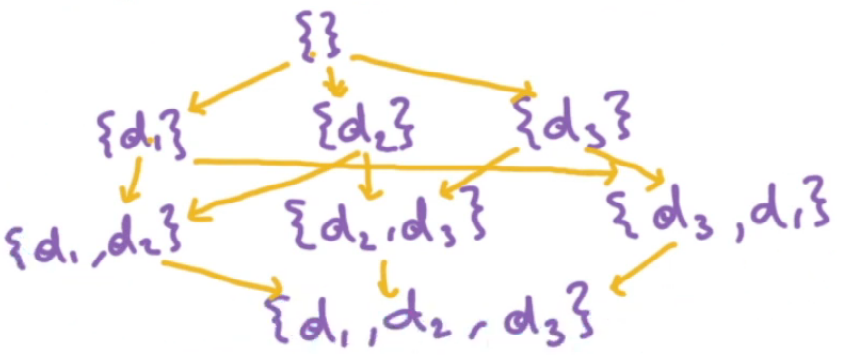
\includegraphics[width=1\linewidth]{images/semilatticeSetUnion.png}
    \caption{Set union semilattice example}
    \label{fig:semilattice_union}
\end{figure}
\begin{figure}[h!]
\caption{Boolean tuples logical AND semilattice example}
\begin{center}
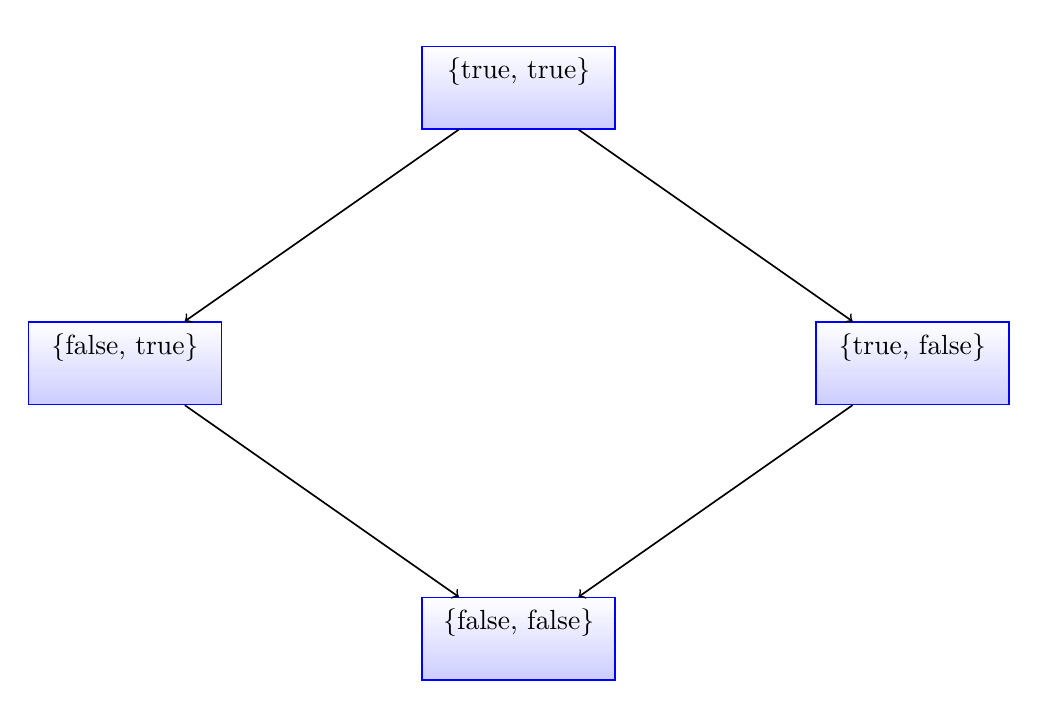
\begin{tikzpicture}[-latex ,auto ,node distance =3.5cm and 5cm ,on grid ,
    semithick ,
    state/.style ={ rectangle ,top color =white , bottom color = blue!20 ,
    draw, blue , text=blue , scale = 0.7 ,minimum width =3.5 cm, minimum height = 1.5 cm}]
    \node[state] (A){} node [label = {}, rectangle split,rectangle split parts=2]{%
      \{true, true\}%
      };
    \node[state] (B) [below left = of A]{} node [label = {},rectangle split,rectangle split parts=2] [below left = of A] {%
      \{false, true\}%
      };
    \node[state] (D) [below right =of A]{} node [label = {},rectangle split,rectangle split parts=2] [below right = of A] {%
      \{true, false\}%
      };
    \node[state] (E) [below left =of D]{} node [label = {},rectangle split,rectangle split parts=2] [below left = of D] {%
      \{false, false\}%
      };
    \path[->] (A) edge node [above = 0.3 cm] {} (D);
    \path[->] (A) edge node [above = 0.3 cm] {} (B);
    \path[->] (B) edge  (E);
    \path[->] (D) edge  (E);
    
\end{tikzpicture}
\end{center}
\label{fig:semilattice_and}
\end{figure}

\subsection{Semilattice properties}
\begin{itemize}
    \item x \^{} y is the first common descendant of x and y.
    \item Define top value T such that x \^{} T = x for all x
    \item Define bottom ($\bot$) such that x \^{} $\bot$ = $\bot$ for all x
    \item Semilattice diagram = picture of partial orders
    
\end{itemize}



% \subsection{Example of \^{} and $\leq$}
% Set-union 
%\subsection{Defining partial order operator $\leq$ through \^{} meet operator}
$a\leq b$ if and only if a \^{} b = a. We can see this in example in figure \ref{fig:semilattice_and}. Consider \{false, true\} and \{true, true\}. The meet operator logical AND gives us \{false, true\}. This satisfies above definition thus \{false, true\} $\leq$ \{true, true\}. 

\subsection{Defining meet operator \^{} through partial order operator $\leq$}
a \^{} b = c if and only if c $\leq$ a, c $\leq$ b and $\nexists$ d d $\leq$ a, d $\leq$ b, c \textless  d. \\
If we are given a partial ordering of values we can always find unique value in the same set which satisfies the above.

\subsection{Semilattice diagram through  $\leq$}
$x\leq y$ indicates that there is a path from x to y and vice versa. This can be observed in figure \ref{fig:semilattice_and}. There may not be a direct edge between two nodes related by partial order operator but there will exist a path.

\subsection{Properties of partial order}
\begin{itemize}
    \item \textbf{Reflexive x $\leq$ x}
    \item \textbf{Anti-symmetric x $\leq$ y and y $\leq$ x $\rightarrow$ x = y}
    \item \textbf{Transitive x $\leq$ y and y $\leq$ z $\rightarrow$ x $\leq$ z}
\end{itemize}
Properties of the meet operator \^{} (idempotent, commutative, associative) guarantee the properties for $\leq$. This can be shown easily.

\subsection{The $<$ operator}
$a<b$ if and only if $a \leq b$ and $b \leq a$. In other words $a\leq b$ and $a\neq b$.

\subsection{Semilattice diagram}
\begin{itemize}
\item \textbf{Set of nodes}: Set of values
\item \textbf{Set of edges}: \{ (y, x) {\textbar} x \textless  y and $\nexists$ z .( x \textless  z and z \textless  y)  \}. If there is such a z then there will be a path from x to z and z to y, so we do not need to draw an edge from x to y.
\end{itemize}

\subsection{Example of \^{} and $\leq$}
\textbf{Meet operator \^{} $\triangleq$ set-union $\cup$} : ((x $\leq$ y) $\triangleq$ (x $\cup$ y = x)) $\equiv$ ( x $\supseteq$ y). Thus x $\leq$ y $\equiv$ ( x $\supseteq$ y).
%\section {Semilattice Representations, Size, Product and Height}
\setlength{\parindent}{0pt}
(Prepared by Shivam Goyal)

\vspace{0.3cm}

\subsection{Semilattice Representation}
\begin{itemize}
    \item \textbf{Set of values $V$ and a meet operator \^{}}
    \item \textbf{Set of values $V$ and a partial order $\leq$}
    \item \textbf{A semilattice diagram} : which is a directed acyclic graph with nodes and edges. It can have potentially multiple Top and Bottom nodes, but they may not necessarily exist for eg in a semilattice with $V$ as set of integers and $max$ as the meet operator
\end{itemize}

\subsection{Semilattice Size}
For some DFA problems, size of the semilattice i.e. the number of elements in the set of values $V$ can become very large. For eg. it could be exponential in number of definitions for a program, if we consider the set of definitions as a value for the semilattice. As the set of values $V$ would be the power set of the set of definitions in the program for some DFA like available expressions.
\subsection{Product of Semilattices}
\begin{itemize}
    \item One idea considering large semilattices is to represent a larger semilattice using product of smaller semilattices.
    \item Consider 2 semilattices with sets of values as $V1$ and $V2$ then we can define a new semilattice as their product.This would contain values in the set $V1$ x $V2$. 
    \item The partial order for the product semilattice would be obtained by applying the respective partial order relations on both the elements of the tuple, i.e. for $\leq$ (the new partial order):
    \par
    ($x_{1}$,$x_{2}$) $\leq$ ($y_{1}$,$y_{2}$) iff $x_{1}$ $\leq_{1}$ $y_{1}$ and $x_{2}$ $\leq_{2}$ $y_{2}$ where $\leq_{1}$ and $\leq_{2}$ are the respective partial orders of the smaller semilattices. 
    \item Similar thing can be done in case of the meet operator with the respective meet operators being applied on each element of the tuple, i.e. for \^{} (the new meet operator):
    \par
    ($x_{1}$,$x_{2}$) \^{} ($y_{1}$,$y_{2}$) $=$ ($x_{1}$ \^{}$_{1}$ $y_{1}$ , $x_{2}$ \^{}$_{2}$ $y_{2}$), where \^{}$_{1}$ and \^{}$_{2}$ are the respective meet operators of the smaller semilattices.
\end{itemize}
 
%\subsection{Height of Semilattice:}
\begin{itemize}
    \item \textbf{Definition}: It is defined as the largest number of greater than($>$) relations that would fit in a descending order.
    \par It can also be defined as the longest path length in the semilattice diagram.
    \item \textbf{Set of values $V$ and a partial order} For eg. in a semilattice with power set of $n$ definitions as the set of values $V$ and set intersection($\cap$) as the meet operator there would be 2\textsuperscript{n} number of elements but the height of the semilattice would be $n$ as that is the maximum path length in the graph(as can be seen in the figure \ref{fig:height_semilattice}). As we go down on each edge the cardinality reduces by 1 and the longest path is from complete set to null set of length $n$.
    \begin{figure}
    \centering
    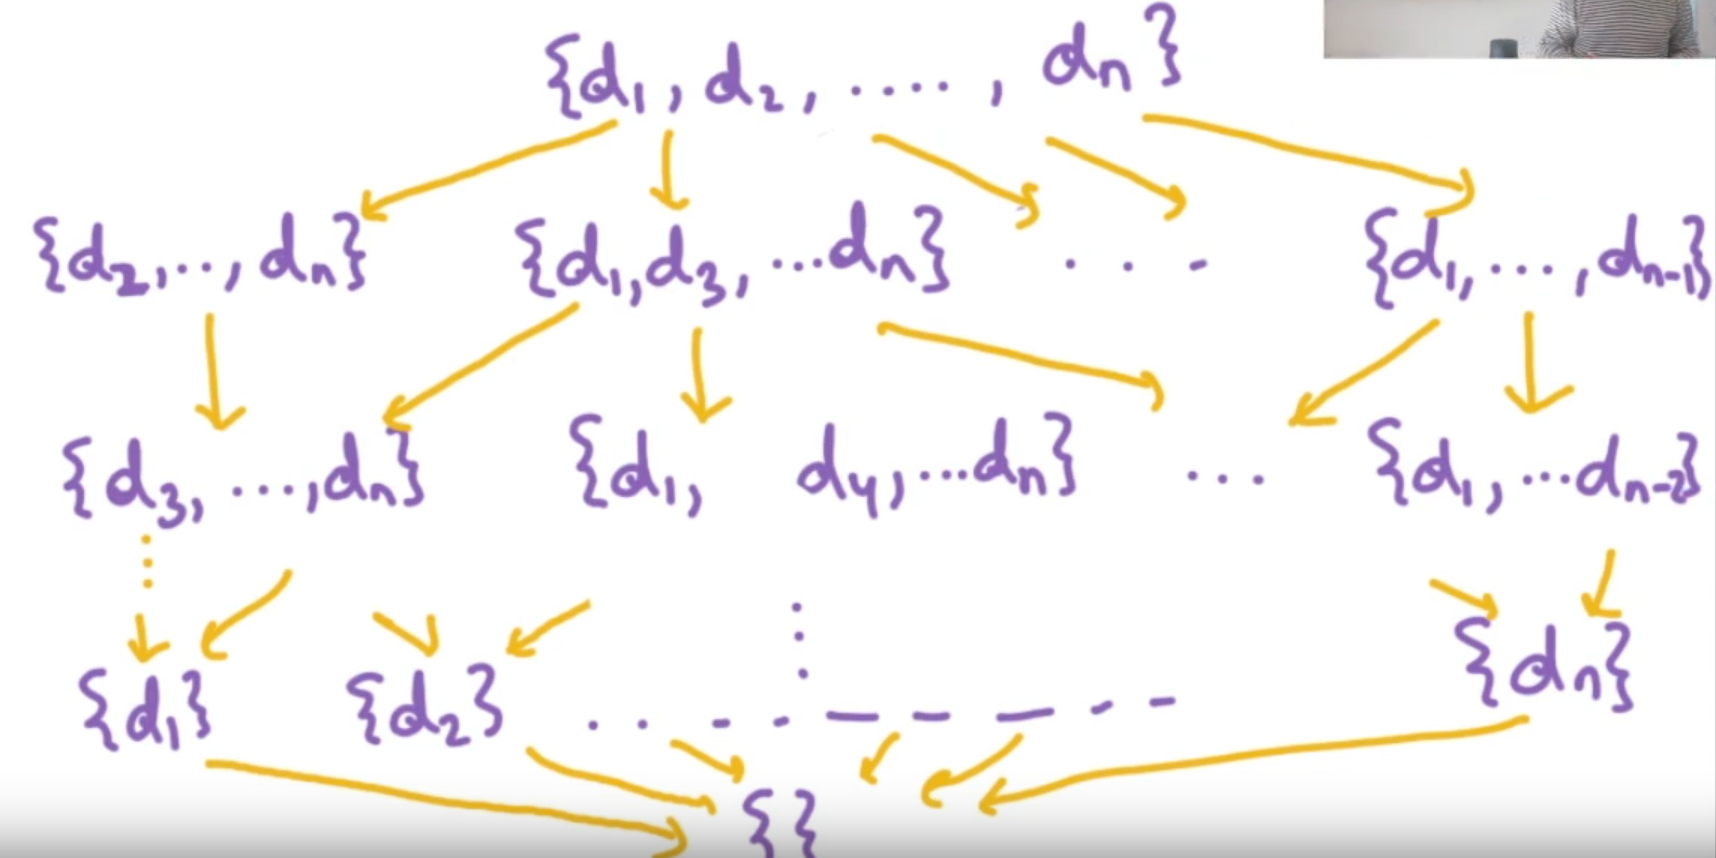
\includegraphics[width=1\linewidth]{images/semilattice_height.png}
    \caption{Semilattice height example}
    \label{fig:height_semilattice}
    \end{figure}
    \par Similarly, for DFA of reaching definitions the height of the semilattice is the number of definitions whereas the number of values is exponential in number of definitions.
    \item Now, There could be infinite height semilattices also having infinite no. of values(eg. set of integers with $max$ as the meet operator) but even with infinite no. of elements in the semilattice it’s height can still be finite, for eg. in case of constant propagation.
    \item Height of the semilattice is an important property because, one of the requirements for the fixed point iteration to converge is that the semilattice height is finite, if it’s infinite then the iteration is not guaranteed to converge.
\end{itemize}

%\section {Family of Transfer Functions}
\setlength{\parindent}{0pt}
(Prepared by Sanket Gandhi)

\vspace{0.3cm}
\begin{itemize}
    \item Recall that a DFA is defined by ($F$, $V$, \^{}) where ($V$, \^{}) forms the semilattice and $F$ is family of transfer functions.
    \item Family of Transfer Functions $F$ is set of functions. For particular DFA each transfer function for an instruction or a basic block is drawn from the set $F$. 
    \item If transfer function does not have certain properties then DFA may not terminate. $F$ should have certain properties in order to reason about optimality and convergence of DFA.
\end{itemize}

\subsection{Properties of Family Transfer Functions F}
Family of transfer functions $F$ must have following properties.  
\begin{itemize}
    \item Every function is $F$ takes a value from DFA value set $V$ and returns a value from same set $V$, that is every function $f$ in $F$ have form $f:V \rightarrow V $
    \item F contains the identity function that is, $\exists \ f \in F \ $ such that $f(x) = x $, $ \forall \ x \in V$. \\ This property is needed because in case of NOP instructions the output is equal to input. So identity function should be in $F$.  
    \item F is closed under composition, if $f_{1},f_{2} \in F$ then $f_{1}\circ f_{2} \in F$.\\ This property will be helpful for defining transfer functions for basic blocks.
\end{itemize}

\subsection{Example}
Many of the DFAs(Reaching definitions, Constant Propagation etc.) have following structure in transfer function.
\[f(x) = (x-kill_{s})\bigcup gen_{s}\] for some instruction $s$. $kill_{s}$ and $gen_{s}$ only depends on $s$ and are independent of $x$.
\\$F$ is the set of function which is populated by changing $kill$ and $gen$ set in above structure.
In case of reaching definitions if we have $n$ definitions in program then size of $F$ will be $4^{n}$.  Lets check whether $F$ is family of transfer functions or not.
\begin{itemize}
    \item Every function in $F$ take a set of some kind $x$ input and perform set operations. The output is also set of same kind. $F$ have first property of family of transfer function.
    \item In case of $gen = \emptyset$ and $kill = \emptyset$, the transfer function will become $f(x) = x$ and $f\in F$.
    \item Consider two functions $f_{1}(x) = (x-kill_{1})\bigcup gen_{1}$ and $f_{2}(x) = (x-kill_{2})\bigcup gen_{2}$. Both $f_{1}, f_{2}$ belongs to $F$. 
    \[f_{2}(f_{1}(x)) = ((x-kill_{1})\bigcup gen_{1}-kill_{2})\bigcup gen_{2}\]
    By using property $A\bigcup B - C = (A-C)\bigcup (B-C)$ the above equation becomes
    \[f_{2}(f_{1}(x)) = (x-(kill_{1} \bigcup kill_{2}))\bigcup ((gen_{1}-kill_{2})\bigcup gen_{2})\]
    With $kill_{1\circ 2} = kill_{1} \bigcup kill_{2}$ and $gen_{1\circ 2} = (gen_{1}-kill_{2})\bigcup gen_{2}$ the composite function becomes $f_{2}(f_{1}(x)) = (x - kill_{1 \circ 2})\bigcup gen_{1\circ 2}$. Therefore $f_{1} \circ f_{2} \in F$ as $F$ contain transfer functions with all possible $gen$ and $kill$ set. 
\end{itemize}
 
%\section {Monotonicity of DFA Framework}
\setlength{\parindent}{0pt}
(Prepared by Sanket Gandhi)

\vspace{0.3cm}
\begin{itemize}
    \item Recall that we require semilatiice ($V$,\^{}) to have finite height with some properties over $F$ to guarantee convergence property of the fixed point  iteration.
    \item Also recall that family of transfer function have three properties, all functions in $F$ should be of form $V$ to $V$, $F$ should contain identity function and $F$ should be closed under composition. Do we have additional requirements from $F$ to guarantee convergence of fixed point iteration?
\end{itemize}

\subsection{Example}
Consider DFA ($F$,$V$,\^{})* with $V = \{true, false\}$, \^{}$= logical \ and $, $F = \{id,not,True,False\}$. The transfer functions are defined as follows:
\[id(x) = x, \ \ \forall x \in V \]
\[not(true) = false\]
\[not(false) = true\]
\[True(x) = true, \ \ \forall x \in V \]
\[False(x) = true, \ \ \forall x \in V \]
\begin{figure}[h!]
\caption{Semilattice diagram of *}
\begin{center}
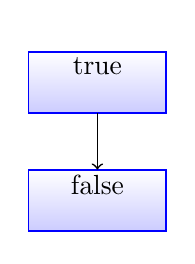
\begin{tikzpicture}[-latex ,auto ,node distance =1.5cm and 2cm ,on grid ,
    semithick ,
    state/.style ={ rectangle ,top color =white , bottom color = blue!20 ,
    draw, blue , text=blue , scale = 0.7 ,minimum width =2.5 cm, minimum height = 1.1 cm}]
    \node[state] (A){} node [label = {}, rectangle split,rectangle split parts=2]{%
      true%
      };
    \node[state] (E) [below =of A]{} node [label = {},rectangle split,rectangle split parts=2] [below = of A] {%
      false%
      };
    \path[->] (A) edge node [above = 0.2 cm] {} (E);
    
\end{tikzpicture}
\end{center}
\label{fig:semilattice_and}
\end{figure}
\begin{itemize}
    \item Note that semilattice have finite height 2.
    \item Every function in $F$ is of form $V \rightarrow V$
    \item $F$ contains the identity function which is $id$.
    \item $F$ is closed under composition
\end{itemize}
The $F$ is valid family of transfer functions. Consider following instance of program. Basic block $B1$ have transfer function $id$ and basic block $B2$ have $not$ transfer function. By boundary condition and initialization of intermediate program point with top value the initial state is also shown in following figure. 
\begin{figure}[ht]
    \centering
    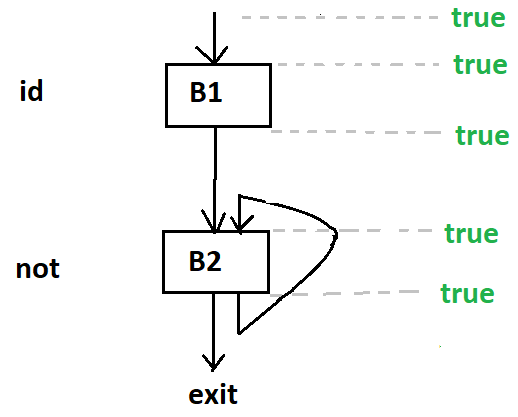
\includegraphics[scale= 0.4]{images/100-1.png}
    \caption{Initial State}
\end{figure}
When iterative fixed point algorithm first time reaches basic block $B2$ it meets over incoming  edges which is logical and of $true$. The out value of $B2$ and hence one of the in edge value of $B2$ become $not(true)$ which is $false$. The meet operator is logical and so the in value of $B2$ also becomes false.
\begin{figure}
    \centering
    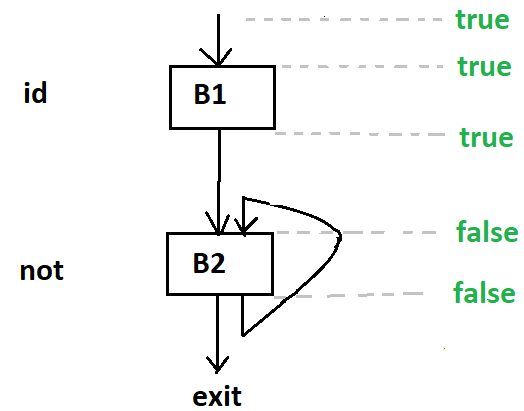
\includegraphics[scale= 0.4]{images/100-2.png}
    \caption{After FPI reaches B2 first time}
\end{figure}
As the $in[B2]$ and $out[B2]$ are not satisfying the transfer function condition FPI will again reach to $B2$. The $in[B2]$ and $out[B2]$ will again become $true$. Even our DFA framework follows all properties discussed earlier the algorithm will never converge. 
\begin{itemize}
    \item There should be some more constraints on family of transfer function $F$ so to guarantee convergence of FPI.  
    \item The problem is $not$ function in $F$ which keeps oscillating between two values. It is expected that the transfer function should keep same order in output values as that of input values(if it is defined).  
\end{itemize}
\subsection{Monotonicity of DFA framework}
A DFA framework ($F$,$V$,\^{}) is monotone if and only if
\[if \ \ \ \ x \leq y \ \ \ implies \ \ \ f(x) \leq f(y) \ \ \ \forall f \in F \ \ \ \ \forall x,y \in V\]
\begin{itemize}
    \item This says that if DFA framework is monotone then for all transfer functions in $F$ if there is particular order in input values then corresponding output values will also follow same order.
    \item In above examples $true \geq false$ but $not(true) \ngeq not(false)$, hence above DFA framework was not monotone.
    \item Equivalently a framework is monotone if and only if $f(x$\^{}$y) \leq f(x)$\^{}$f(y)$.
    The proof for DFA monotonicity implies $f(x$\^{}$y) \leq f(x)$\^{}$f(y)$ was provided in live session and is as follows:\\
    \textit{Proof:} By definition of meet operator,
    $a$\^{}$b \leq a$ and  $a$\^{}$b \leq b$. As DFA framework is monotone for all tansfer functions $f(a$\^{}$b) \leq f(a)$ and $f(a$\^{}$b) \leq f(b)$ holds. Now $f(a$\^{}$b) \leq f(b)$ implies $f(a$\^{}$b)$\^{}$f(b) = f(a$\^{}$b)$. Similarly $f(a$\^{}$b) \leq f(a)$ implies $f(a$\^{}$b)$\^{}$f(a) = f(a$\^{}$b)$. Now consider $(f(a)$\^{}$f(b))$\^{}$f(a$\^{}$b)$ is same as as $(f(a)$\^{}$f(b))$\^{}$(f(a$\^{}$b)$\^{}$f(a$\^{}$b))$. By using properties of meet operator the above expression is same as 
    $(f(a)$\^{}$f(a$\^{}$b))$\^{}$(f(b)$\^{}$f(a$\^{}$b))$. Which further boils down to $f(a$\^{}$b)$\^{}$f(a$\^{}$b)$ = $f(a$\^{}$b)$. At the end $(f(a)$\^{}$f(b))$\^{}$f(a$\^{}$b)$ = $f(a$\^{}$b)$. Therefore $f(a)$\^{}$f(b) \geq f(a$\^{}$b)$.
    \item Also in example discussed above $not(false$\^{}$true) = true$ and $not(true)$\^{}$not(false)=false$. Which means $not(false$\^{}$true) \nleq not(false)$\^{}$not(true)$ and so DFA framework in example was not monotone.

\subsection{Monotone DFA Example}
Consider the reaching definitions DFA ($F$,$V$,\^{}). The transfer function in this framework is of type $f(x) = (x-kill)\bigcup gen$. The values in this framework are set of definitions. If $x\leq y$ then this implies $x \supseteq y$ for $x,y \in V$. For transfer function $f\in F$ and $x_{1},x_{2} \in V$,
\[f(x_{1}) = (x_{1}-kill)\bigcup gen\]
\[f(x_{2}) = (x_{2}-kill)\bigcup gen\]
Clearly if $x_{1} \leq x_{2}$ implies $x_{1} \supseteq x_{2}$ which implies $f(x_{1}) \supseteq f(x_{2})$. This implies $f(x_{1}) \leq f(x_{2})$. This shows ($F$,$V$,\^{}) is monotone. 
\end{itemize}
%\include{../module101} 
%\include{../module102}
%\include{../module103} 
%\include{../module104}
%\section{Partial Redundancy Elimination}
\begin{flushright}
\textit{Notes by Akshin Singh}
\end{flushright}

IN PROGRESS 
%\section{Lazy Code Motion Problem}
\begin{flushright}
\textit{Notes by Akshin Singh}
\end{flushright}

As discussed in the previous module, the PRE problem has two components
\begin{enumerate}
\item All redundant computations of expressions that can be eliminated without duplication are eliminated.
\item The optimized program does not perform any extra computations that were not in the original program \textit{execution}.
\end{enumerate}

Lazy Code Motion (or LCM for short) adds another component to it.

\begin{enumerate}
  \setcounter{enumi}{2}
\item Expressions are computed at the late as possible (this is where the name \textbf{LAZY} comes from).
\end{enumerate}


\begin{figure}[h]
\centering
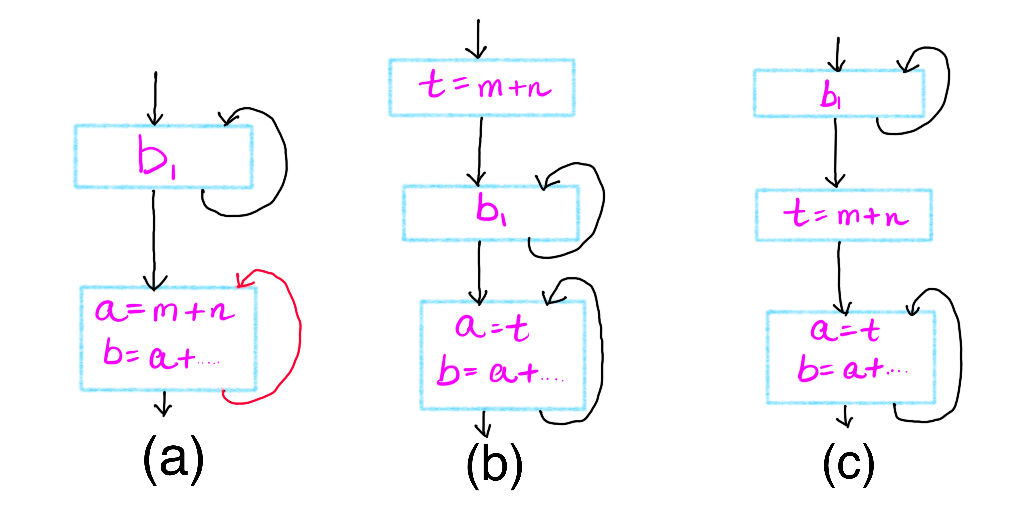
\includegraphics[scale = 0.5]{images/mod_106_fig1.png}
\caption{Lazy Code Motion example}
\label {fig:mod_106_01}
\end{figure}

Let us understand this with the help of an example. In Figure \ref{fig:mod_106_01}(a), we see that \textbf{m+n} is redundant on the red path,i.e., the loop's back edge. We will formally define what a back edge means in a later module. For now, the back edge means the edge that takes the execution from the loop's body back to its body.

PRE allows \ref{fig:mod_106_01}(b) but LCM does not. \textbf{WHY?} For PRE, components 1 and 2 are satisified in \ref{fig:mod_106_01}(b). For LCM component 3 is not satisfied. We can see this from the fact that the loop consisting of b1 needs to hold the value of \textbf{m+n} even though it does not need it. LCM component 3 is satisfied in \ref{fig:mod_106_01}(c).

Notice how \ref{fig:mod_106_01}(c) is a solution for both LCM and PRE whereas \ref{fig:mod_106_01}(b) is a solution for PRE but not LCM. This example suggests that $PRE \subset LCM$. In other words, LCM subsumes PRE. This is expected since PRE shares both its rules with LCM, but LCM has extra conditions as well.

\subsection{Full vs Partial Redundancy}

As eluded to in the last module, an expression is fully redundant at a program point if it is redundant on all paths to that program point. If an expressions is redundant on some but not all paths, then that expression is partially redundant.

Another way to frame what PRE does is the following: \textit{Can we place additional copies of an expression e which is partially redundant at program point p, such that it becomes fully redundant at p?} A fully redundant expression can be easily eliminated using common subexpression elimination.


\textbf{For more examples see the lecture module 106 on YouTube}.




%\section{Lazy Code Motion Algorithm}
\begin{flushright}
\textit{Notes by Akshin Singh}
\end{flushright}

IN PROGRESS 
%\include{../module108}
%\include{../module109} 
%\include{../module110}
%\include{../module111} 
%\include{../module112}
%\include{../module113} 
%\include{../module114}
%\include{../module115} 
%\include{../module116}
%\include{../module117} 
%\include{../module118}
%\include{../module119} 
%\include{../module120}
%\include{../module121} 
%\include{../module122}
%\include{../module123} 
%\include{../module124}
%\include{../module125} 
%\include{../module126}
%\include{../module127} 
%\include{../module128}
%\include{../module129} 
%\include{../module130}
%\include{../module131} 
%\include{../module132}
%\include{../module133} 
%\include{../module134}
%\include{../module135} 
%\include{../module136}
%\include{../module137} 
%\include{../module138}
%\include{../module139} 
%\include{../module140}
%\include{../module141} 
%\include{../module142}
%\include{../module143} 
%\include{../module144}
%\include{../module145} 
%\include{../module146}
%\include{../module147} 
%\include{../module148}
%\include{../module149} 
%\include{../module150}
\end{document}
